\documentclass[compress=false,usepdftitle=false, subsection=false,xcolor=dvipsnames]{beamer}
%
%
\usetheme{LMU}
\setbeamercovered{dynamic} % shows items in white grey before active
\setbeamertemplate{caption}{\raggedright\insertcaption\par} % don't show "figure 1" in caption
%
% -----------------------------------------------------------------------------
%
\usepackage[utf8x]{inputenc}
\usepackage{amsmath}
\usepackage{amssymb}
%\usepackage{mathrsfs}
\usepackage{mathtools}
\usepackage{graphicx}
\usepackage{tikz}
\usepackage{tcolorbox}
\usepackage{xcolor}
\usepackage{anyfontsize}
%

% -----------------------------------------------------------------------------
%
\pdfpageattr {/Group << /S /Transparency /I true /CS /DeviceRGB>>}
%
% -----------------------------------------------------------------------------
%
%\setcounter{tocdepth}{2}
%\stepcounter{subsection}
%
\patchcmd{\slideentry}{\advance\beamer@xpos by1\relax}{}{}{}
\def\beamer@subsectionentry#1#2#3#4#5{\advance\beamer@xpos by1\relax}%

% -----------------------------------------------------------------------------
%

\title[]{\textbf{Passive monitoring using traffic noise recordings - case study on the Steinachtal Bridge}}
%\subtitle{}
\author[Johannes Salvermoser]{Johannes Salvermoser, C{\'e}line Hadziioannou, Simon C. St{\"a}hler}
\date{17.03.2016}
\institute{Institute for Earth and Environmental Sciences\\ Ludwig Maximilians University Munich}
%
% -----------------------------------------------------------------------------
%
\hypersetup{%
pdftitle    = {DGG 2016},
pdfsubject  = {},
pdfauthor   = {Johannes Salvermoser},
pdfkeywords = {}}
%
% -----------------------------------------------------------------------------
%
\graphicspath{{../Pics/}}
\setbeamertemplate{navigation symbols}{}
%
% =============================================================================
\begin{document}
% =============================================================================
%
\frame{\titlepage}
%
% =============================================================================
%
%\begin{frame}
%\begin{figure}
%\includegraphics[width=0.85\textwidth]{./pics/title.png}
%\end{figure}
%\end{frame}
%
% =============================================================================
%
\section{Overview}
\subsection{Overview}

\begin{frame}
    \begin{center}
        \begin{tikzpicture}
            \node[anchor=center] at (0,0) {\begin{small}
            	\begin{tcolorbox}[colback=green!5,colframe=salve@blue,title=\textbf{Objective}, width=9cm]{Is it possible to use ambient and/or traffic noise to monitor small-scale structures?}
					\end{tcolorbox}
            	\end{small}
            	};
        \end{tikzpicture}
    \end{center}
\end{frame}

\begin{frame}\frametitle{Motivation}
    \begin{center}
        \begin{tikzpicture}[overlay]
            \node[anchor=south west, inner sep=0] (box) at (-5,1) {\begin{tcolorbox}[colback=green!5,colframe=red, width=10cm]{Issue: Combination of \textbf{precise} and \textbf{permanent} monitoring with a \textbf{simple} measurement setup and evaluation technique.}
					\end{tcolorbox}
            	};
            	\node[anchor=south west, inner sep=0] (fig) at (-4.2,-4) {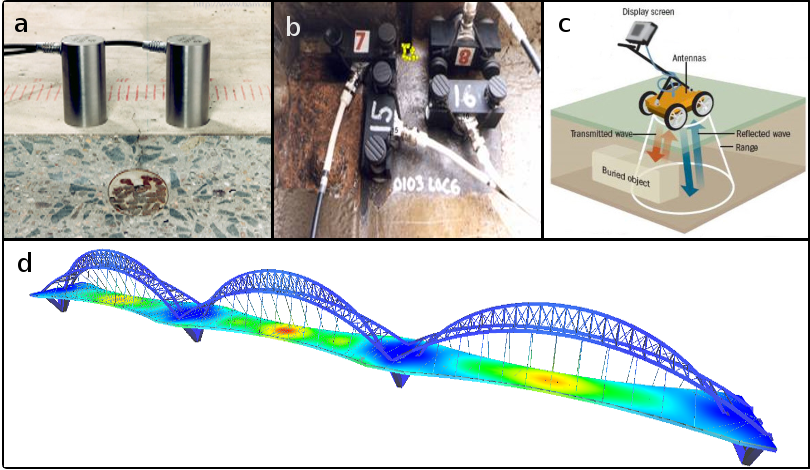
\includegraphics[width=.7\textwidth]{Figures/NDT_methods.png}};
        \end{tikzpicture}
    \end{center}
\end{frame}
% =============================================================================
%


\section{Setup}


\subsection{Setup}
\begin{frame}\frametitle{Measurement Setup I}
    \begin{center}
        \begin{tikzpicture}
            \node[anchor=south west,inner sep=0] (image) at (0,0.5) {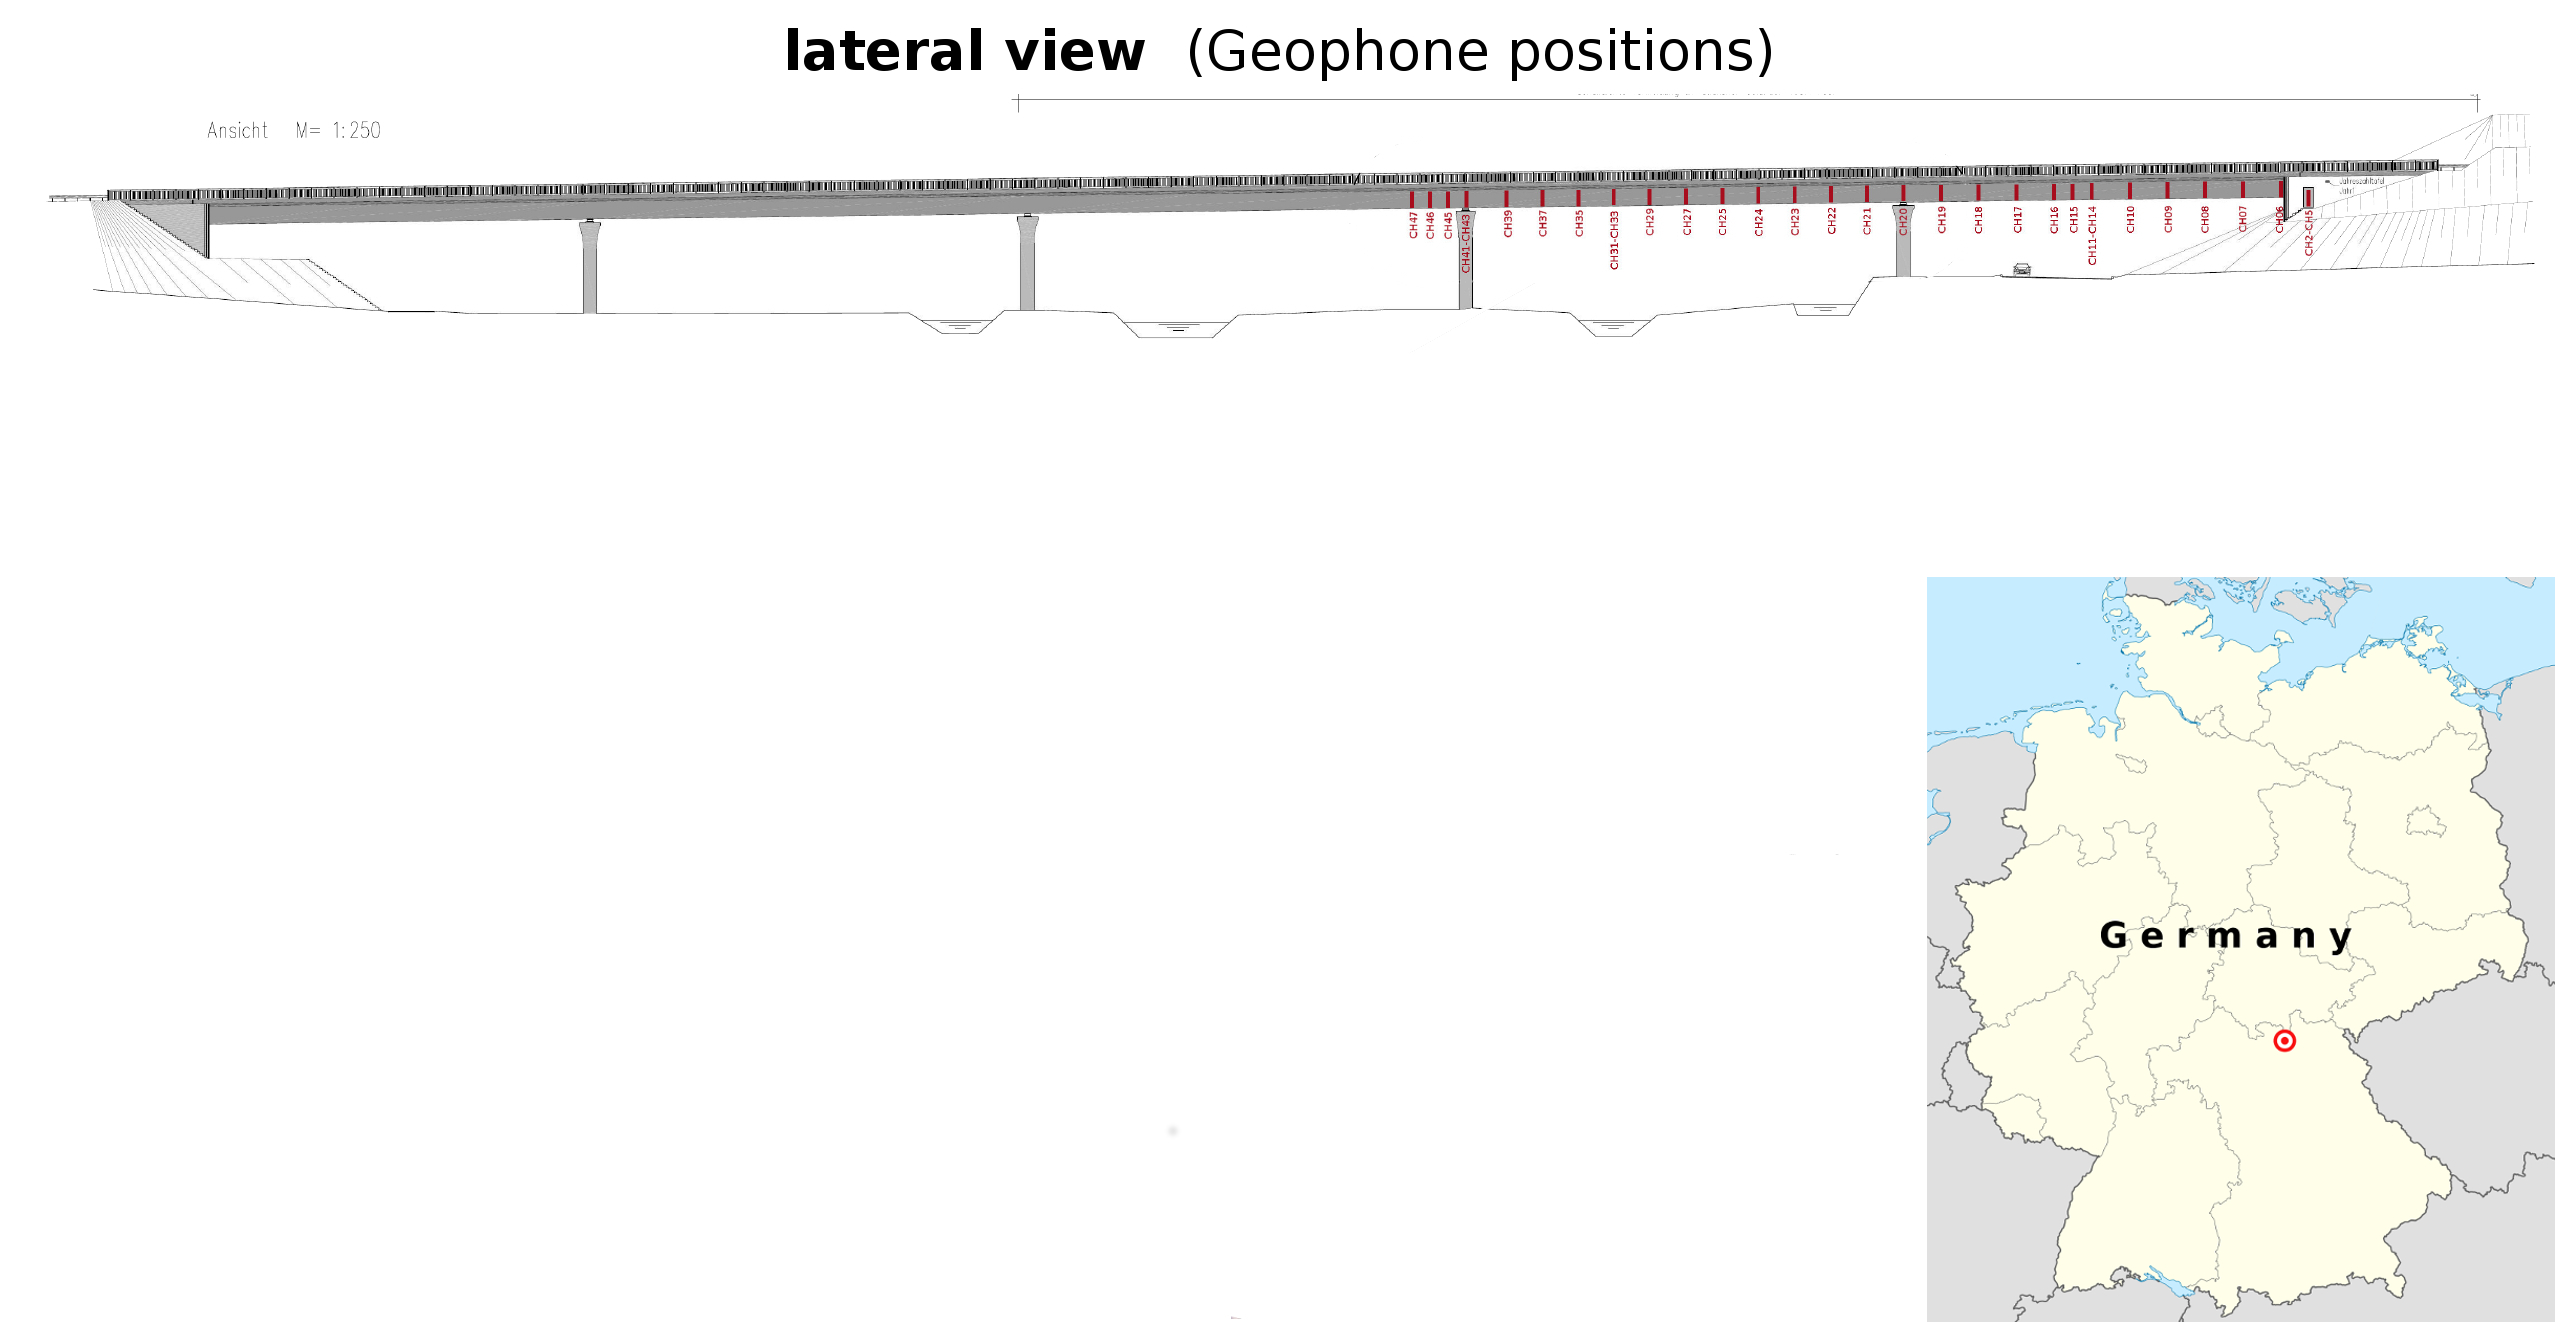
\includegraphics[width=\textwidth]{Figures/setup1.jpg}};
            \node[align=center] at (7.4,1.0) {};
        \end{tikzpicture}
    \end{center}
\end{frame}


\begin{frame}\frametitle{Measurement Setup I}
    \begin{center}
        \begin{tikzpicture}
            \node[anchor=south west,inner sep=0] (image) at (0,0.5) {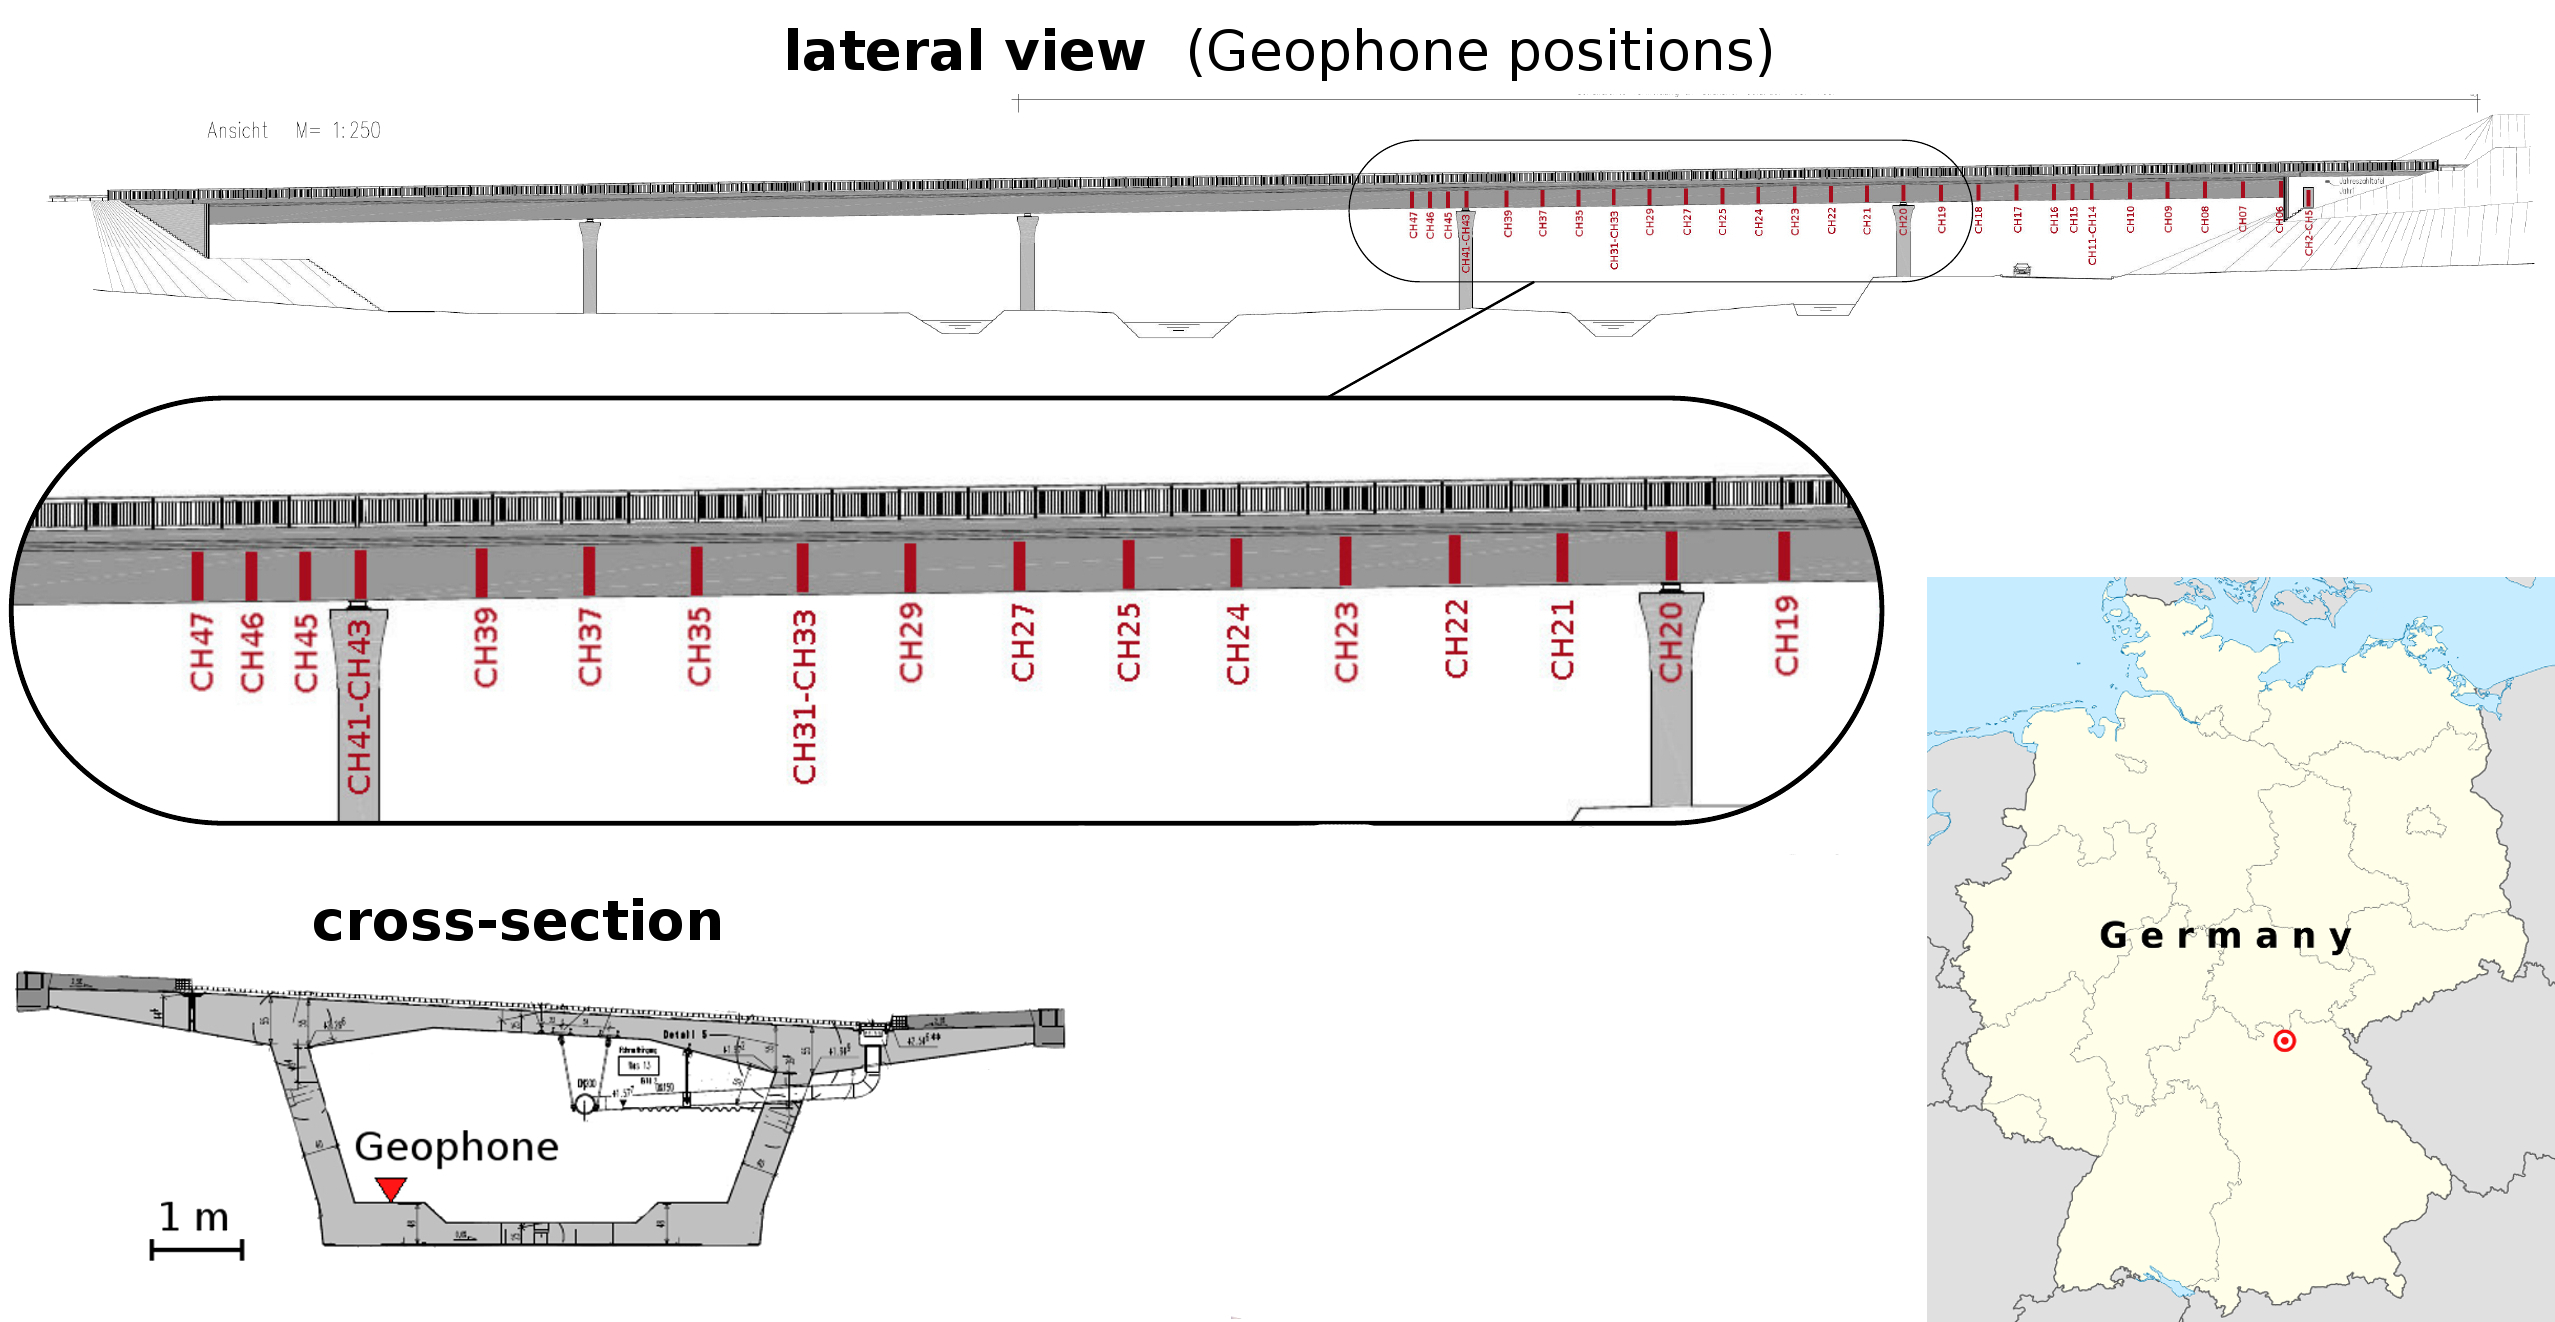
\includegraphics[width=\textwidth]{Figures/setup2.jpg}};
            \node[align=center] at (7.4,1.0) {};
        \end{tikzpicture}
    \end{center}
\end{frame}


% =============================================================================

\subsection{Setup}
\begin{frame}\frametitle{Measurement Setup II: Steinachtal Bridge}
    \begin{center}
        \begin{tikzpicture}
            \node[anchor=south west,inner sep=0] (image) at (-5,4) {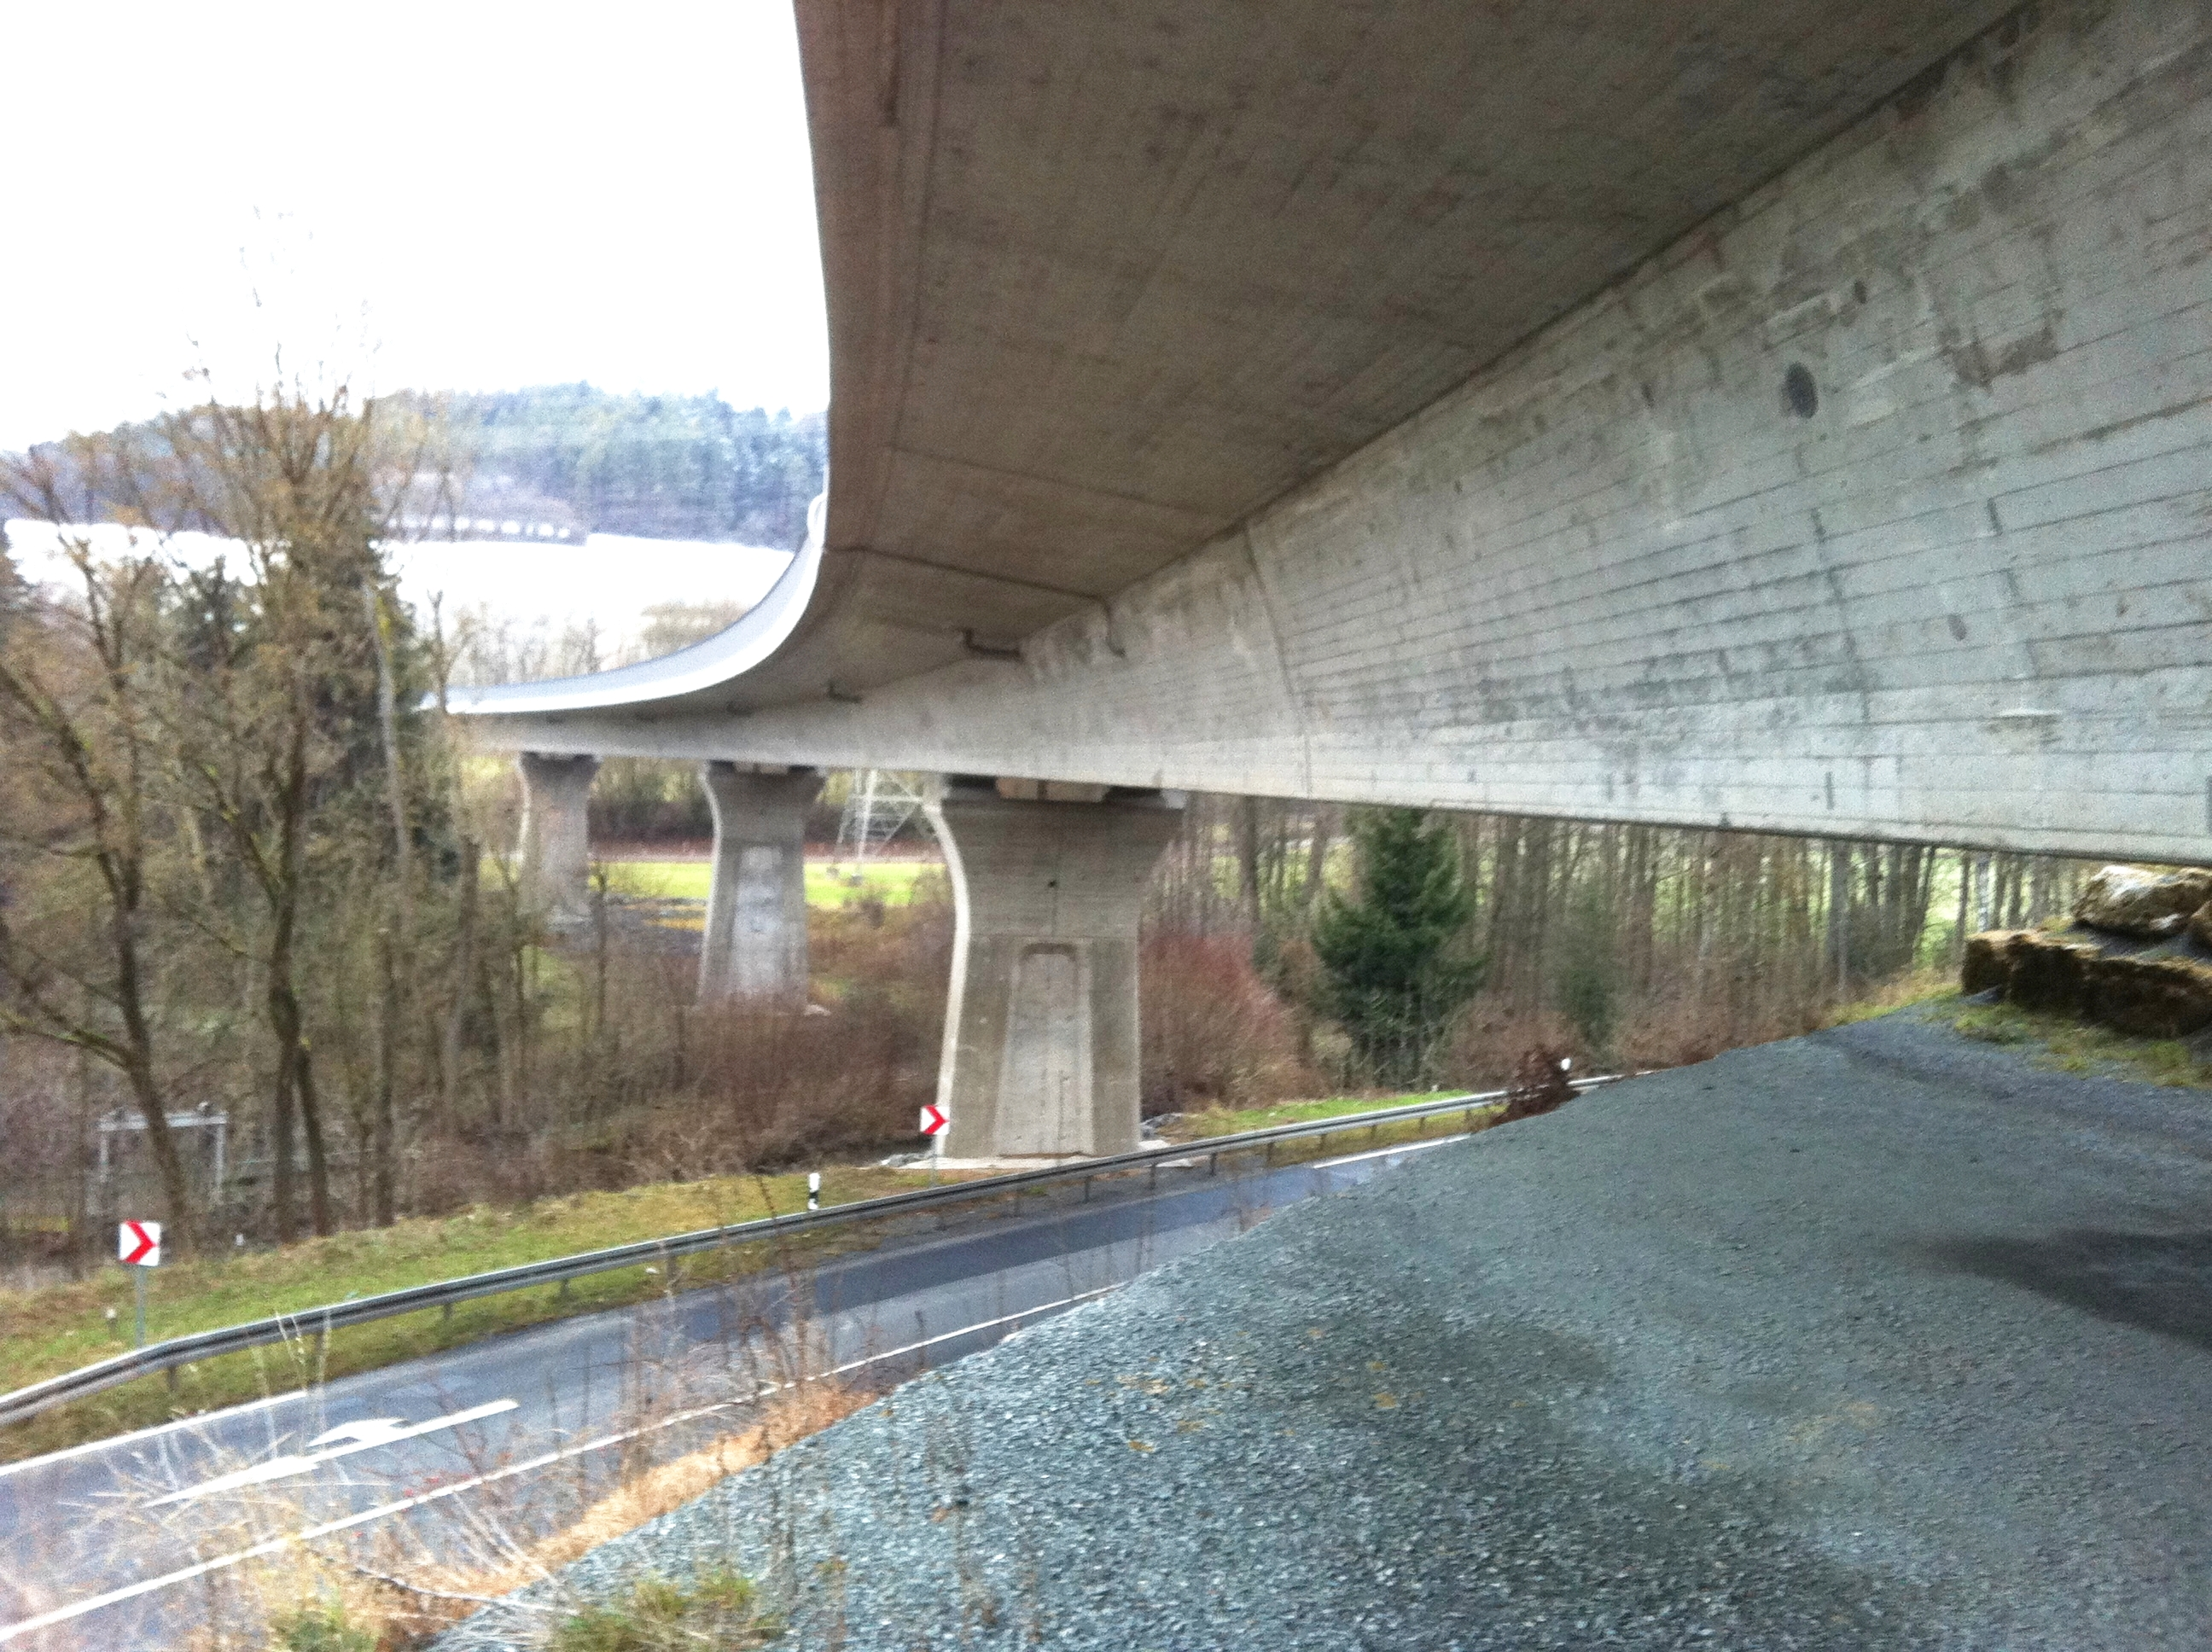
\includegraphics[width=0.55\textwidth]{Figures/bridge_outside2.JPG}};
            \node[anchor=south west, inner sep=0] at (2,2.5) {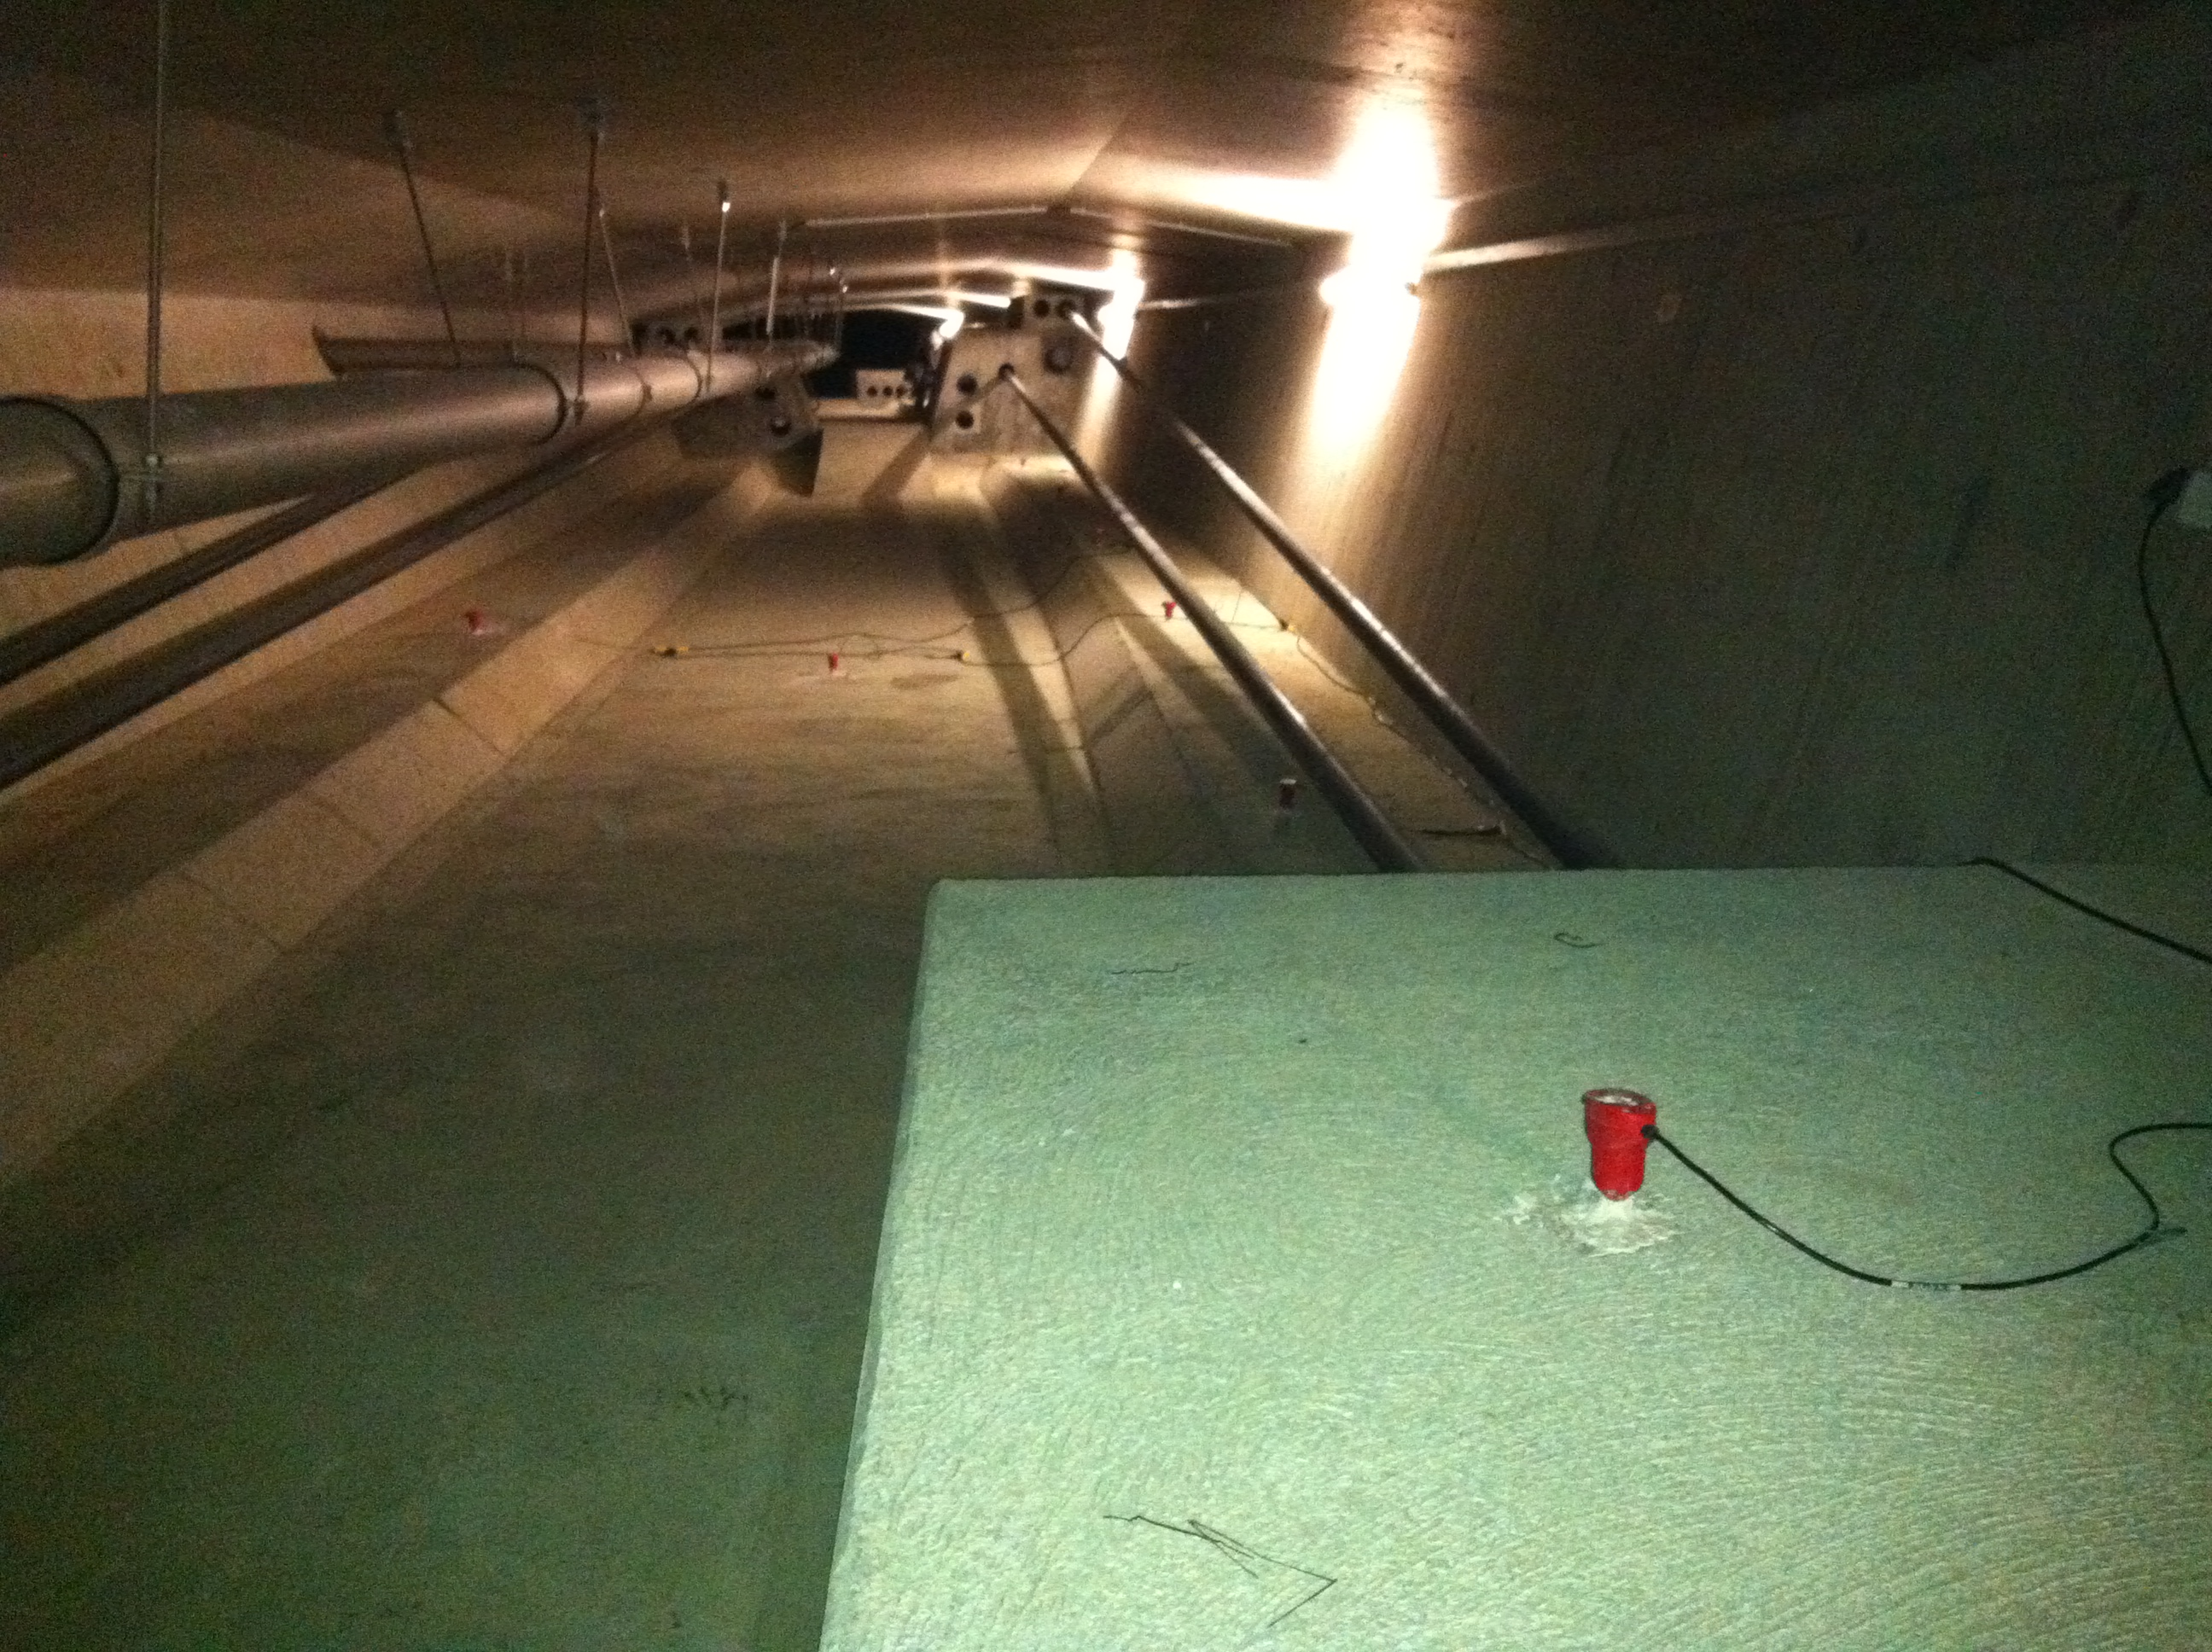
\includegraphics[width=0.36\textwidth]{Figures/overview.JPG}};
            \node[anchor=south west, inner sep=0] at (3,6) {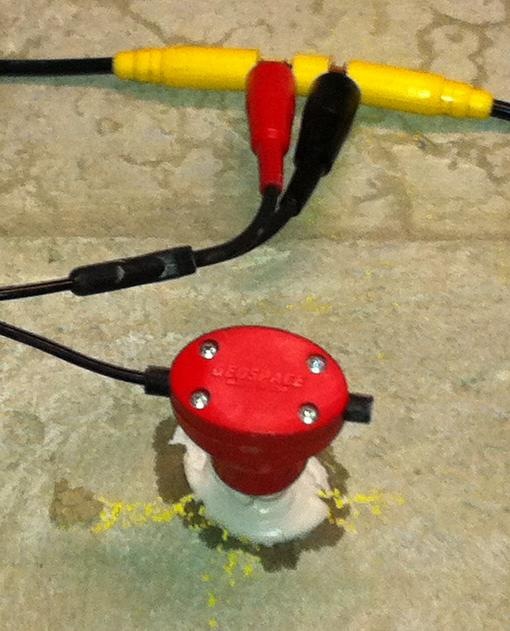
\includegraphics[width=0.2\textwidth]{Figures/Geophone.JPG}};
        \end{tikzpicture}
    \end{center}
\end{frame}
%
% =============================================================================
%

\section{Raw}
\subsection{Raw}
\begin{frame}{bla}\frametitle{Raw Signal}
	\begin{center}
        \begin{tikzpicture}
            \node[anchor=south west,inner sep=0] (image) at (0,0) 	  
            	 {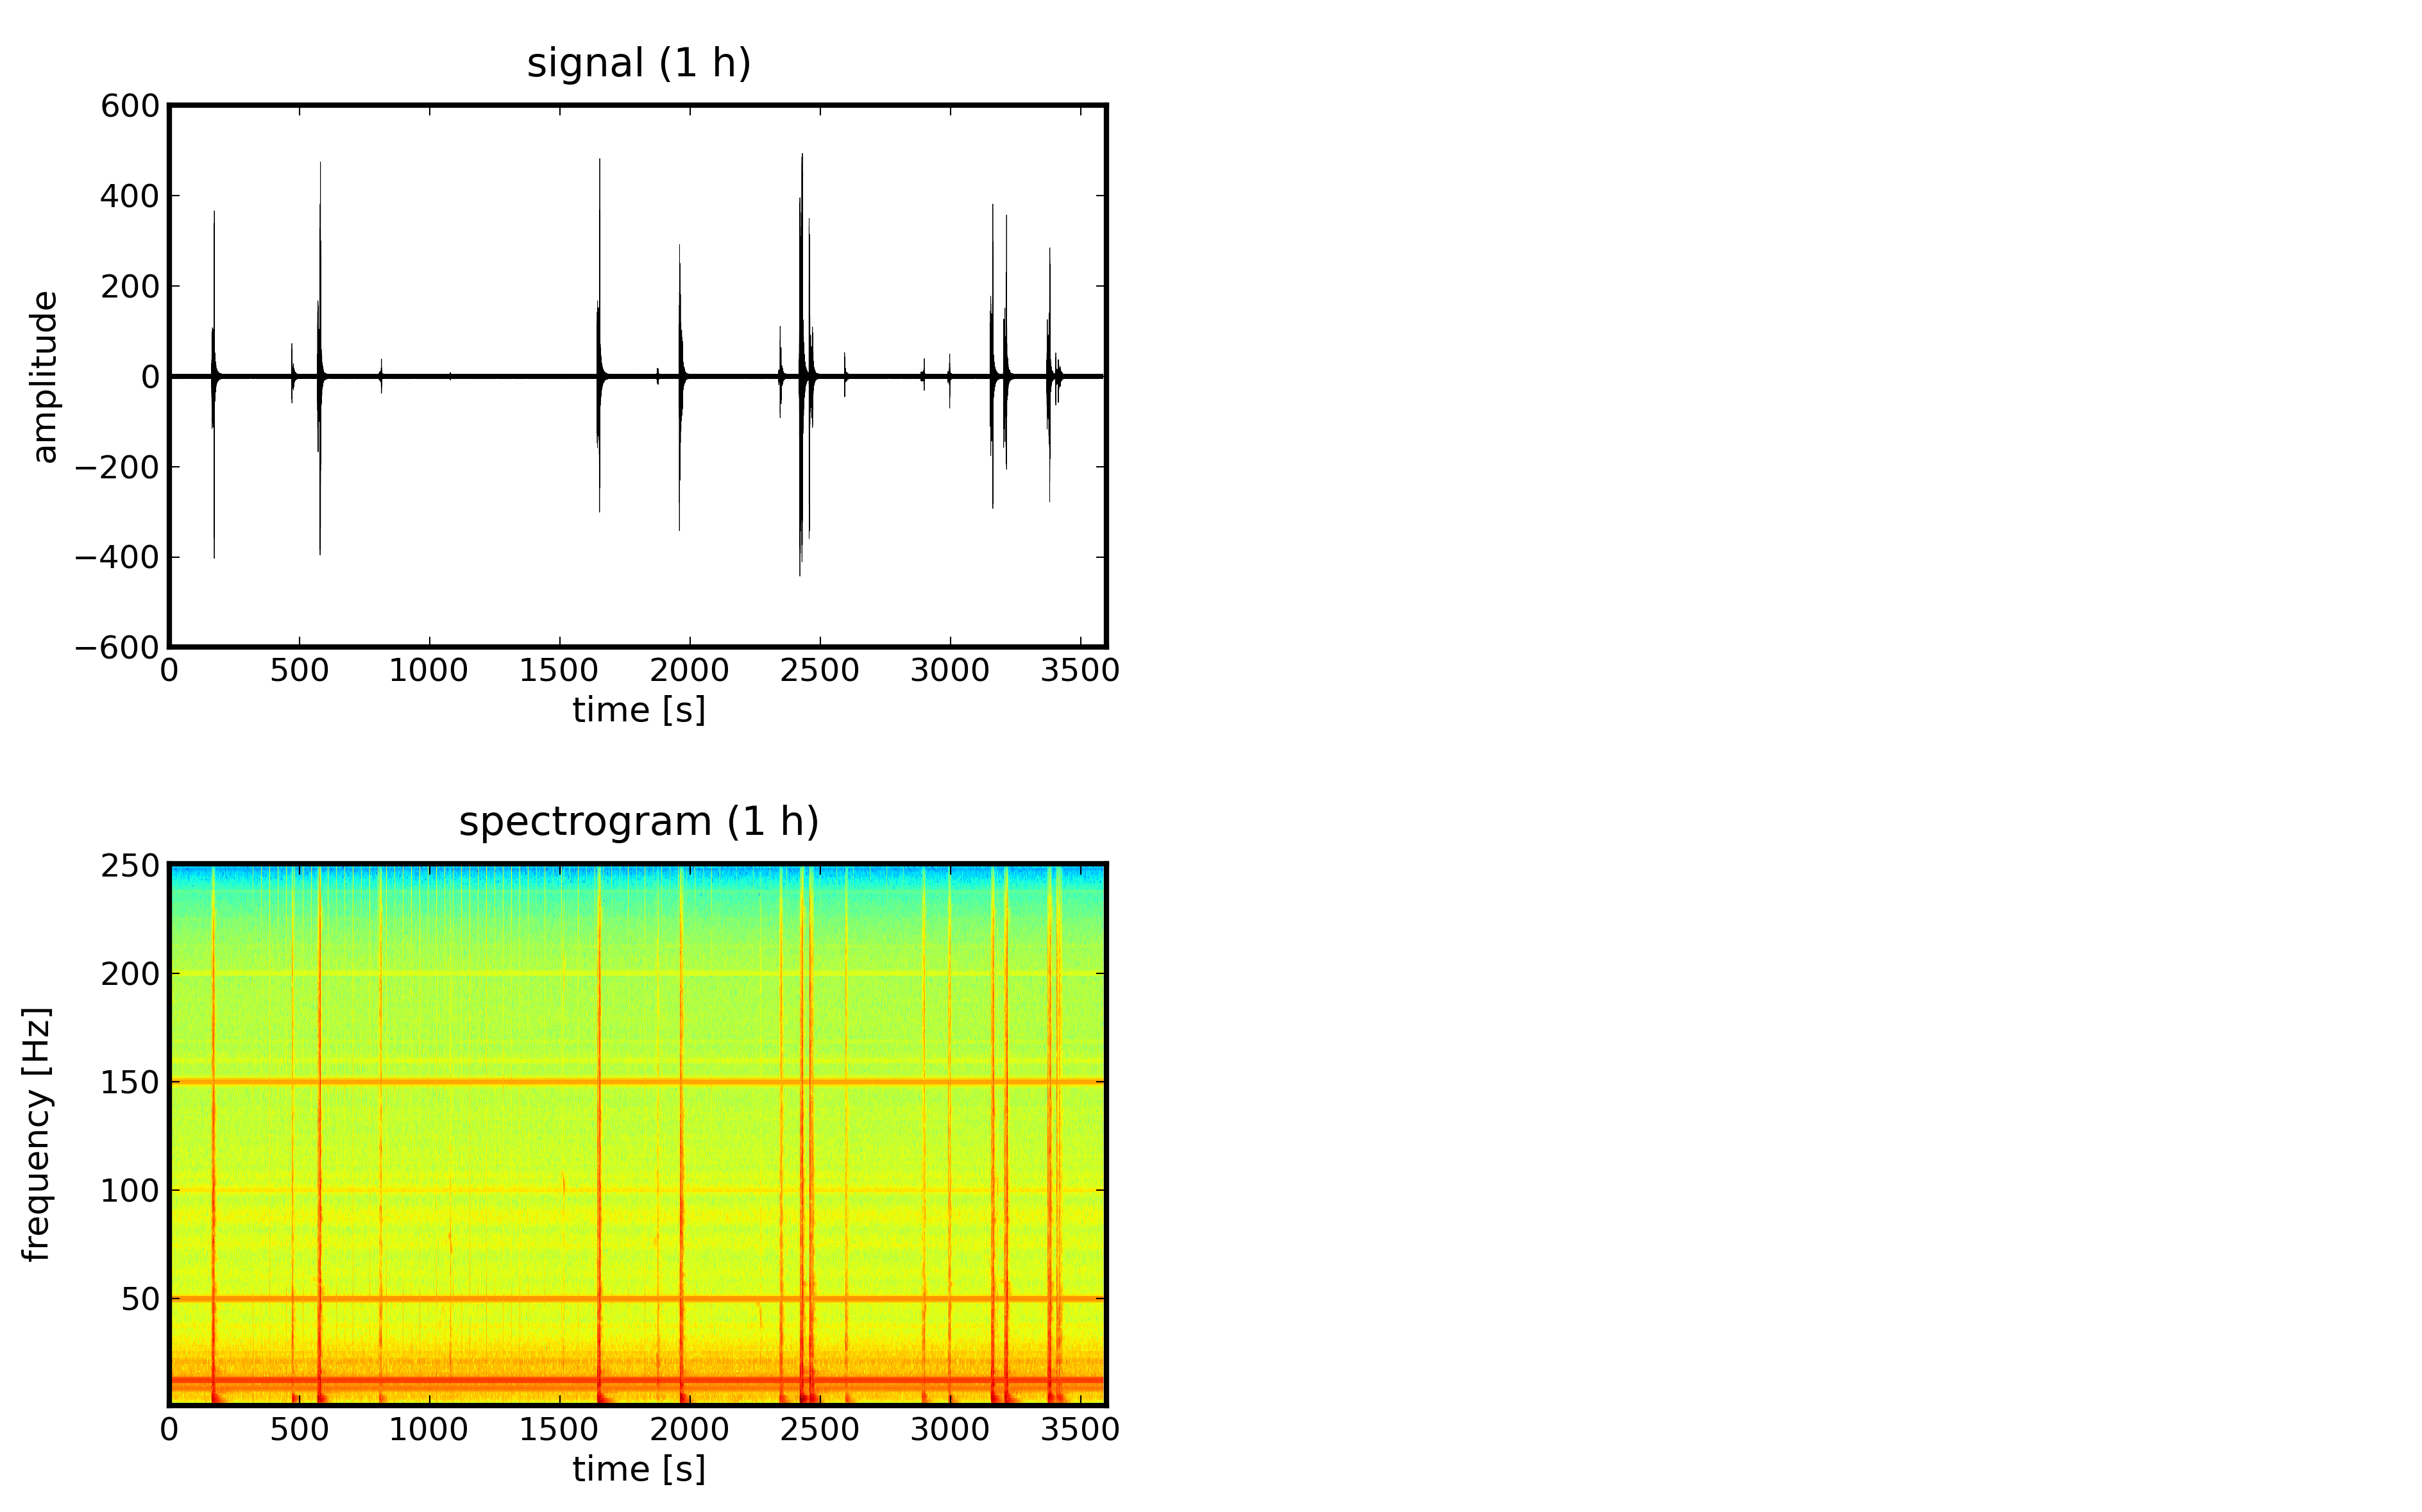
\includegraphics[width=\linewidth,height=0.89\textheight,keepaspectratio]{Figures/raw1.png}};
            \node[align=center] at (image.center) {};
        \end{tikzpicture}
    \end{center}
\end{frame}

\begin{frame}{bla}\frametitle{Raw Signal}
	\begin{center}
        \begin{tikzpicture}
            \node[anchor=south west,inner sep=0] (image) at (0,0) 	  
            	 {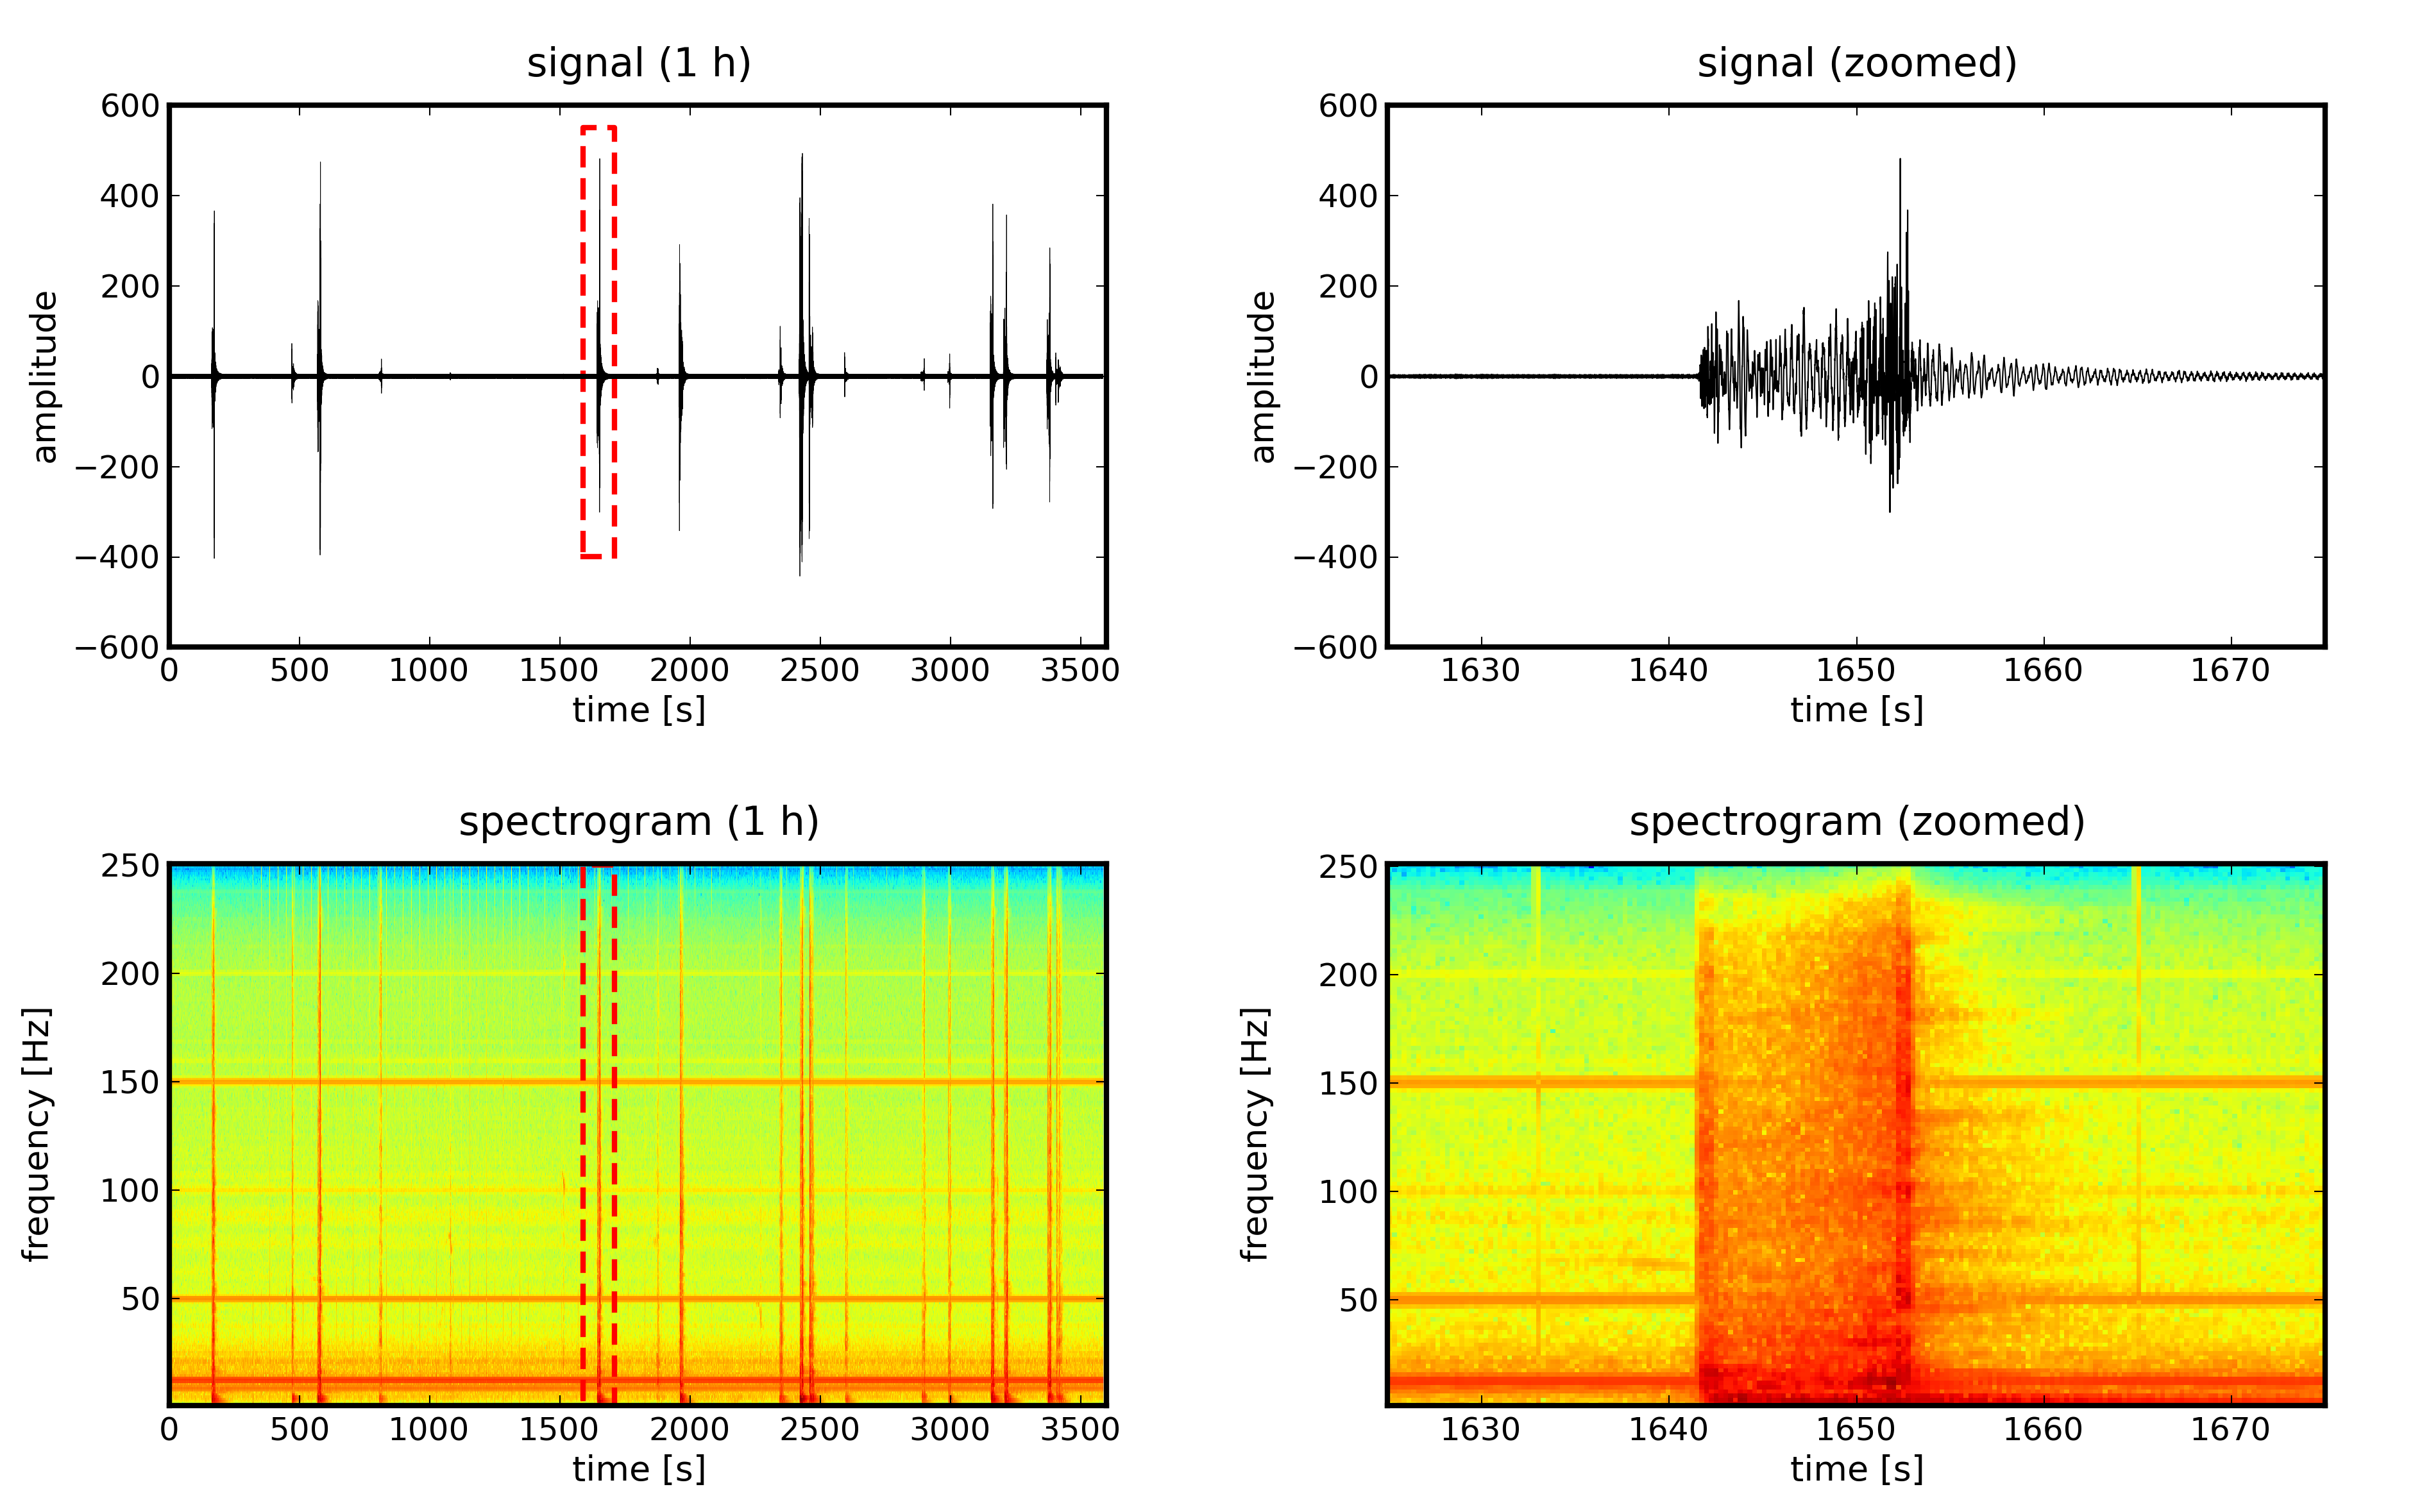
\includegraphics[width=\linewidth,height=0.89\textheight,keepaspectratio]{Figures/raw2.png}};
            \node[align=center] at (image.center) {};
        \end{tikzpicture}
    \end{center}
\end{frame}

\begin{frame}{bla}\frametitle{Raw Signal}
	\begin{center}
        \begin{tikzpicture}
            \node[anchor=south west,inner sep=0] (image) at (0,0) 	  
            	 {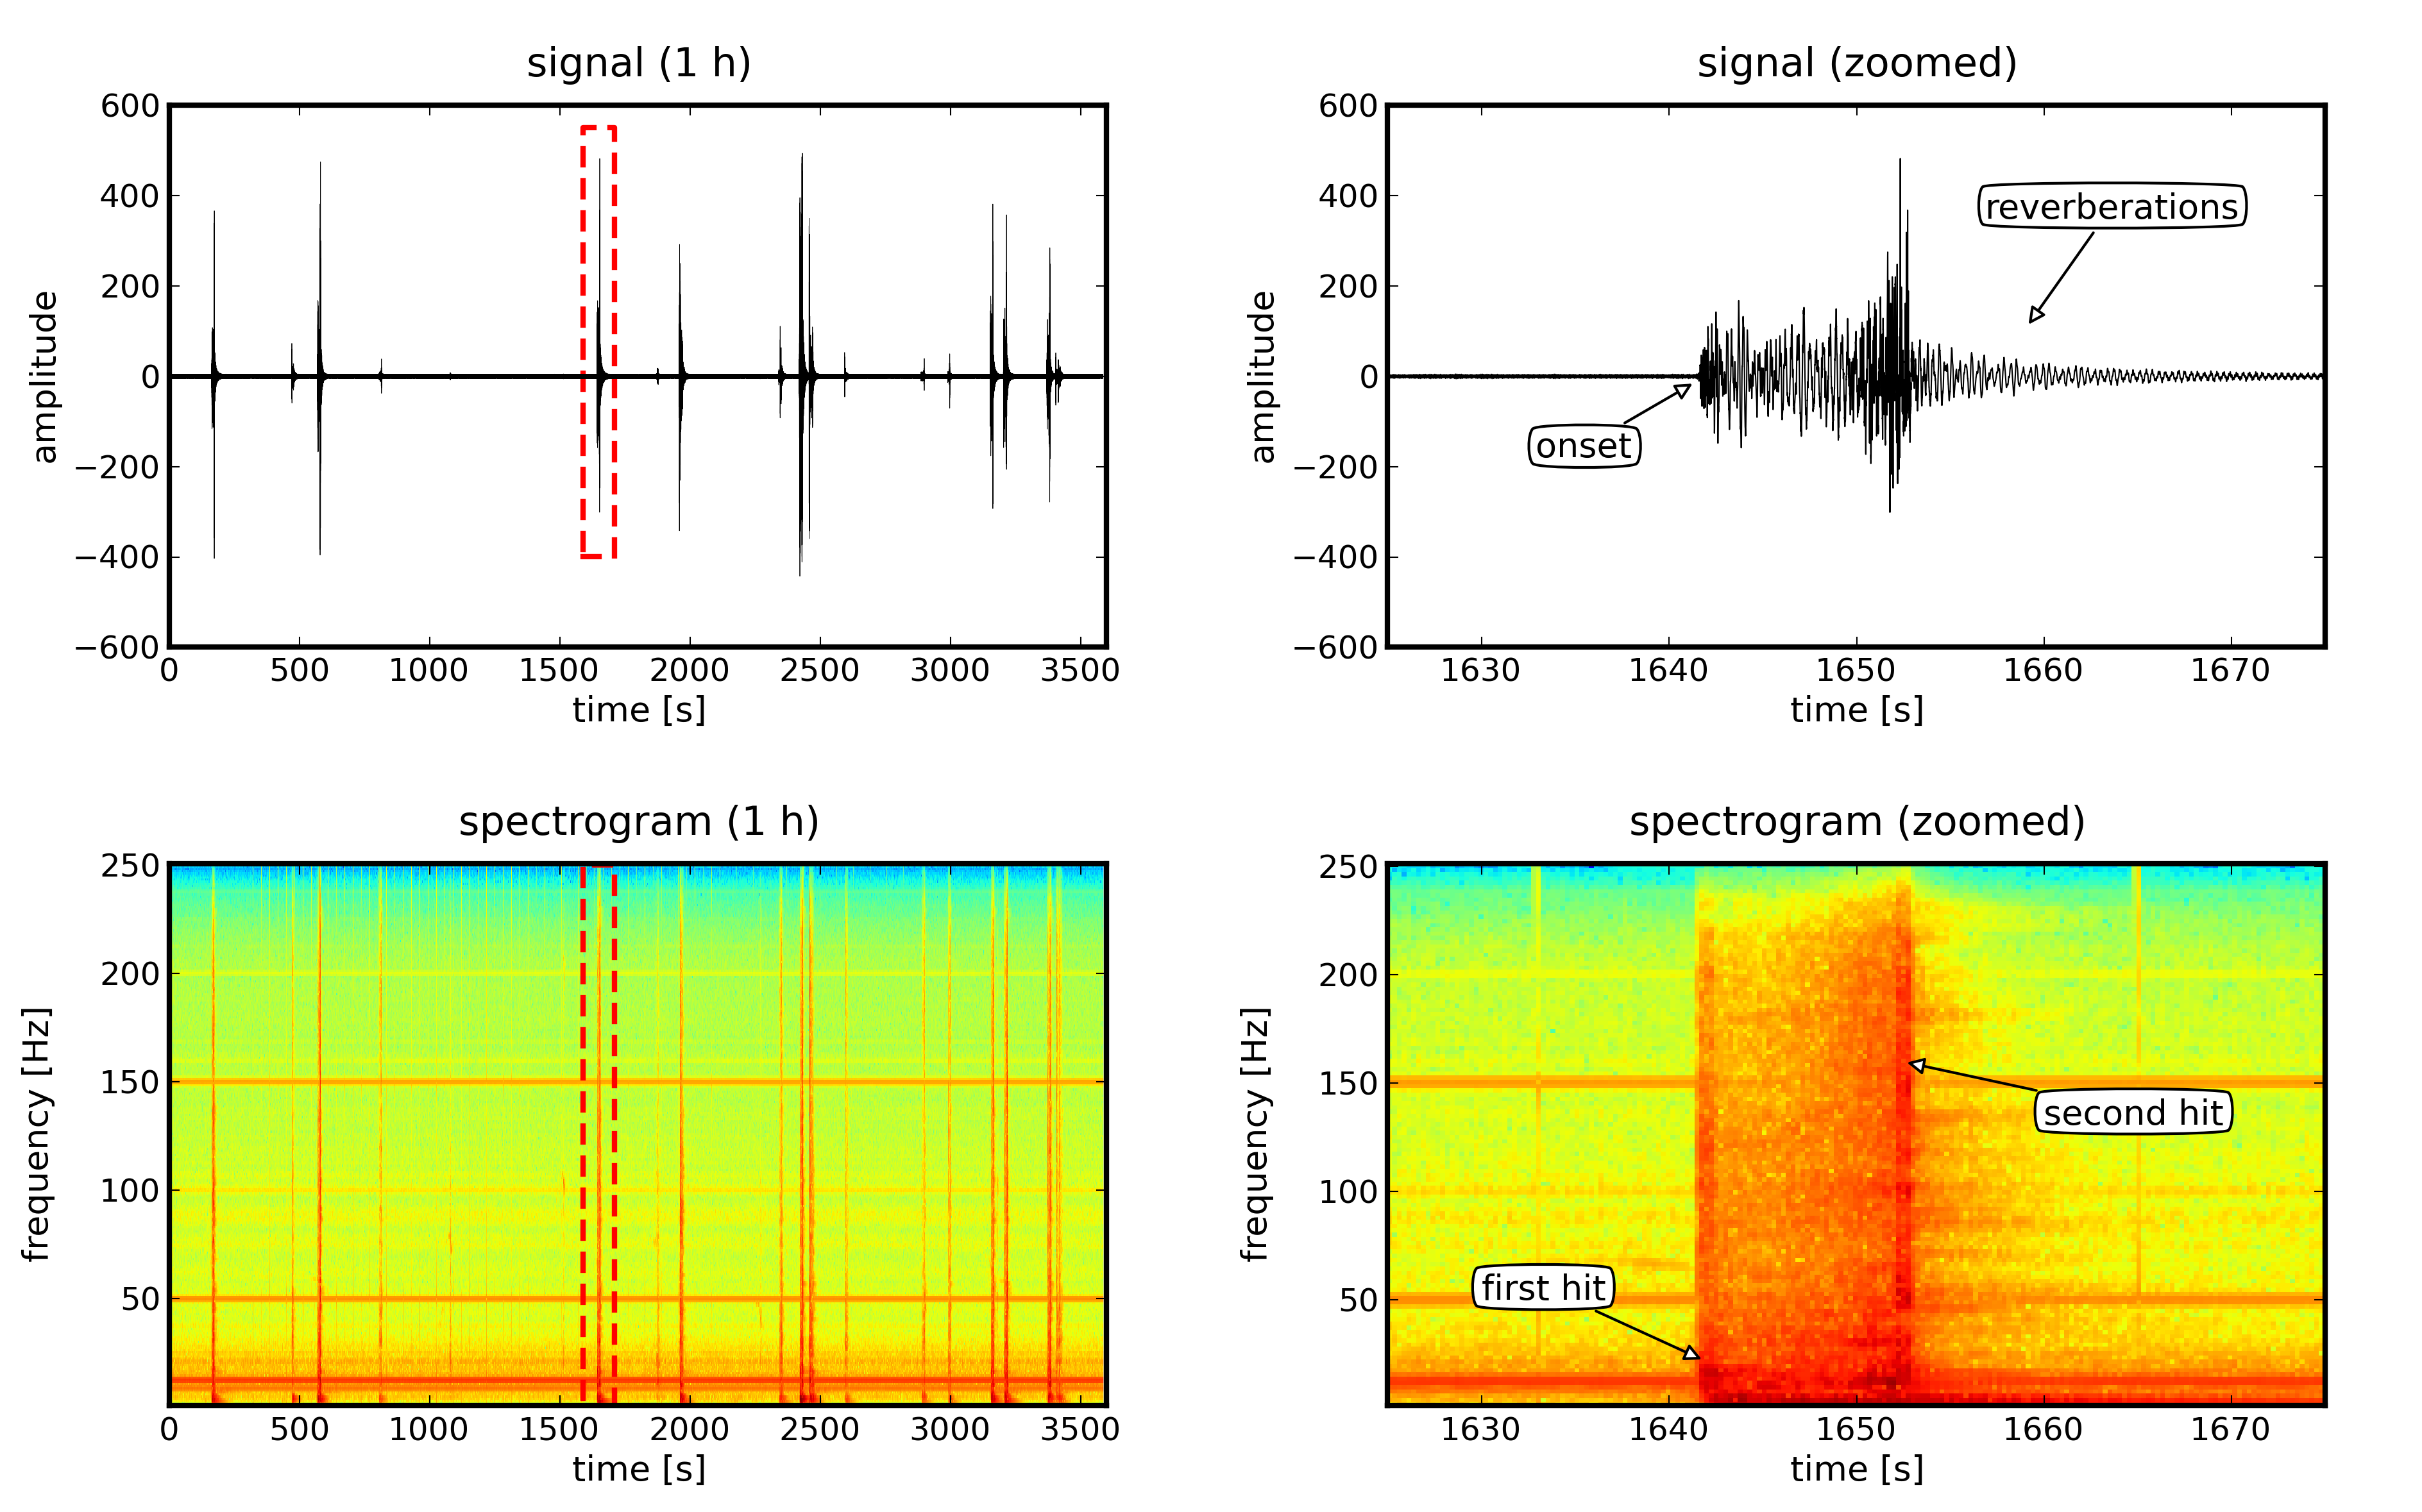
\includegraphics[width=\linewidth,height=0.89\textheight,keepaspectratio]{Figures/raw2+arrows.png}};
            \node[align=center] at (image.center) {};
        \end{tikzpicture}
    \end{center}
\end{frame}

\begin{frame}{bla}\frametitle{Raw Signal}
	\begin{center}
        \begin{tikzpicture}
            \node[anchor=south west,inner sep=0] (image) at (0,0) 	  
            	 {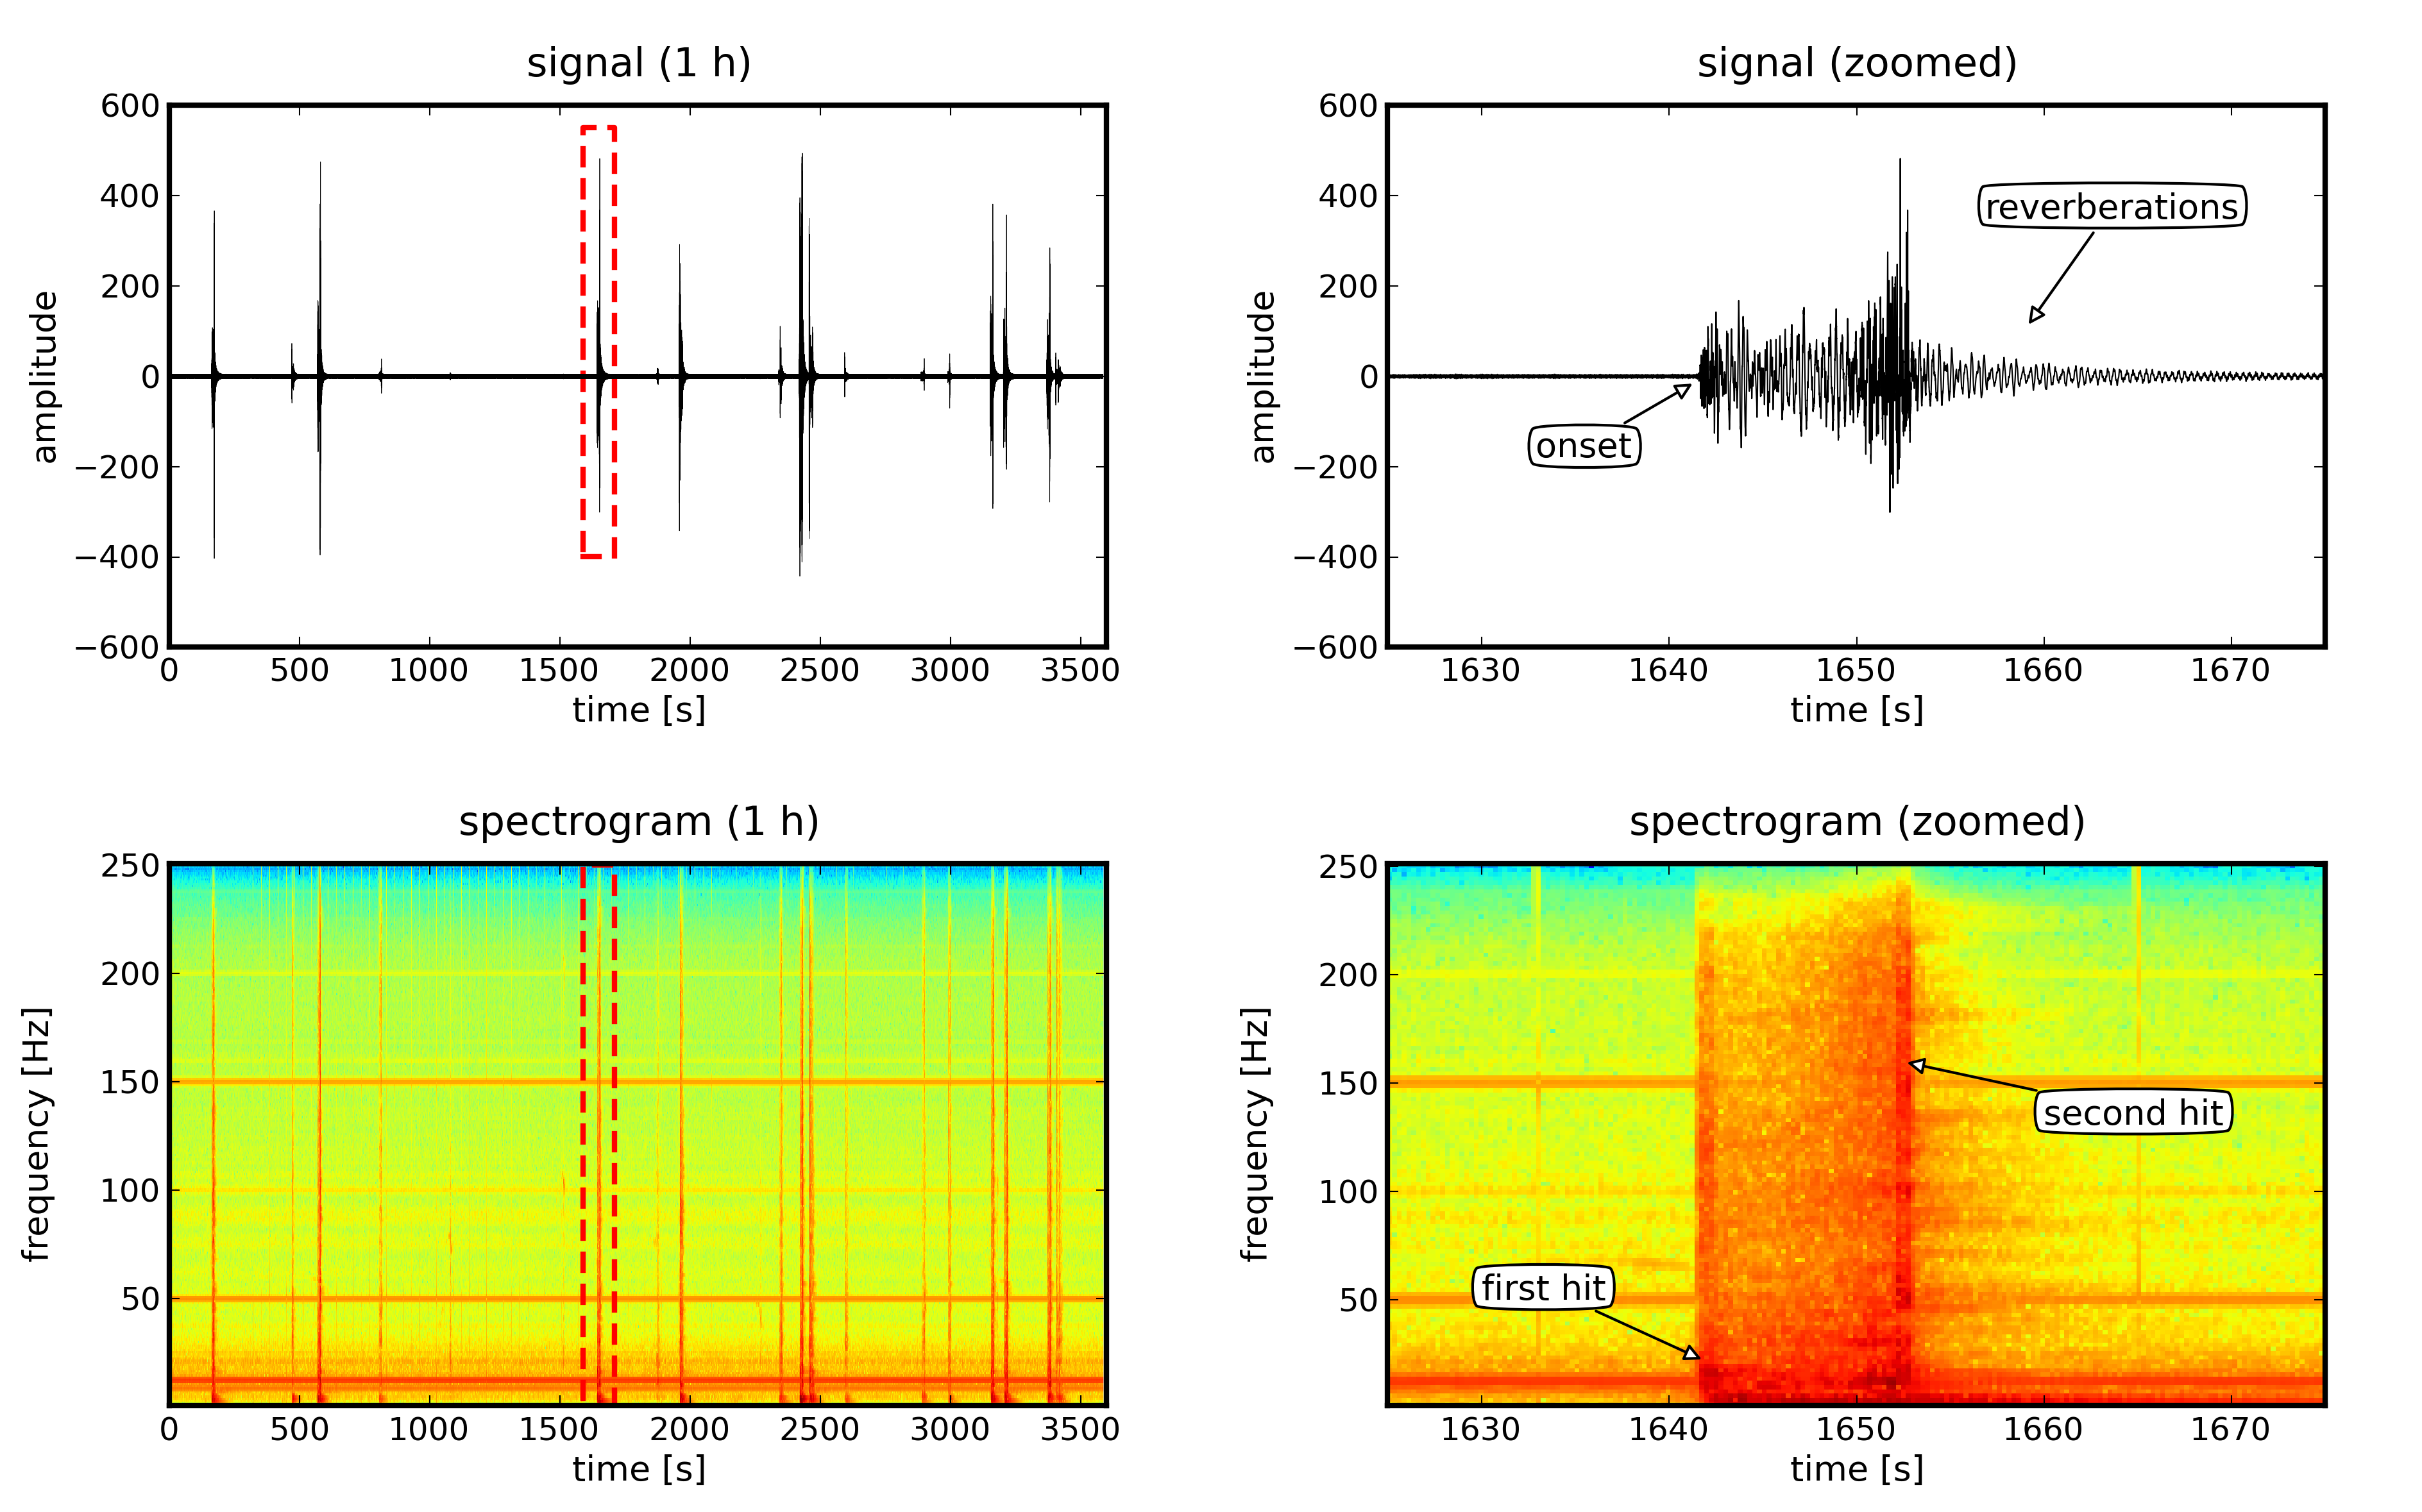
\includegraphics[width=\linewidth,height=0.89\textheight,keepaspectratio]{Figures/raw2+arrows.png}};
            \node[align=center] at (image.center) {};
            \node[anchor=center] at (image.center) {
            		\begin{tcolorbox}[colback=green!5,colframe=salve@blue,title=Spectrum {\color{salve@blue} (filtered)}, width=7cm]
						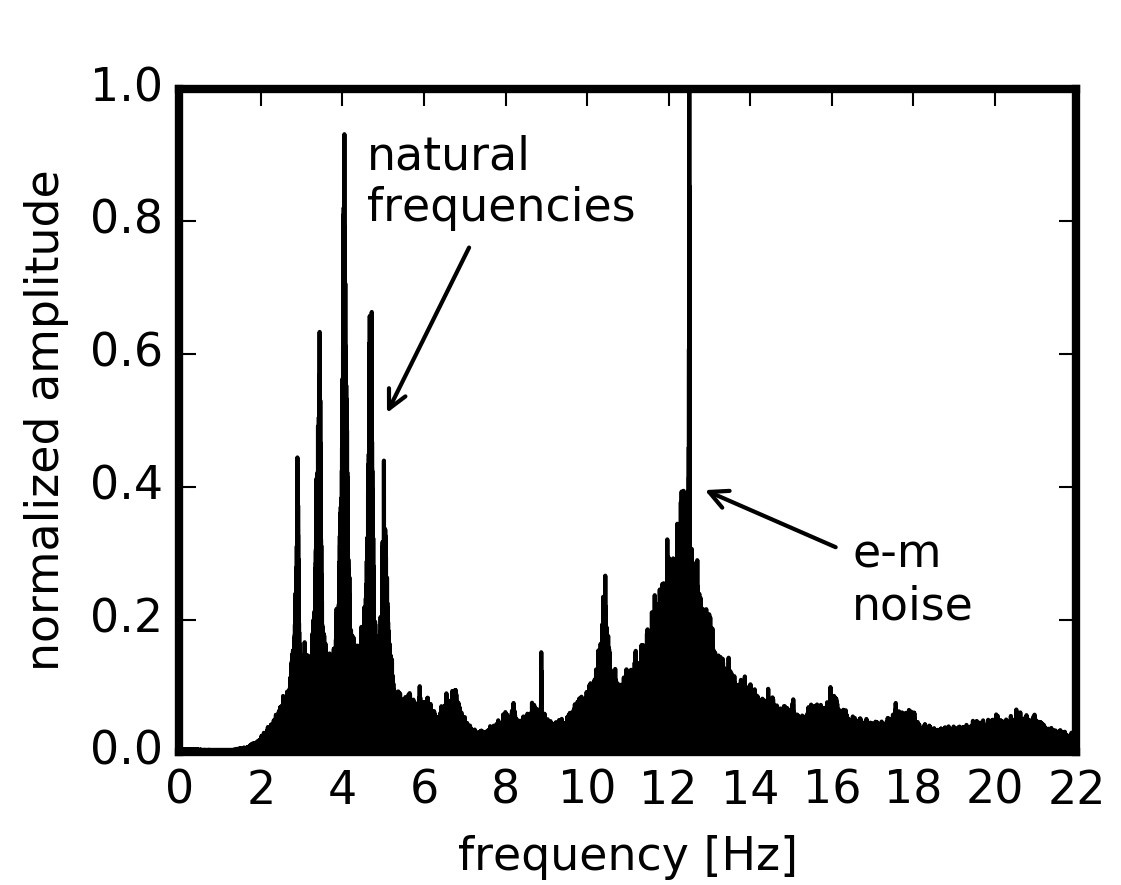
\includegraphics[width=\textwidth]{Figures/spectrum1.png}
					\end{tcolorbox}
            };
        \end{tikzpicture}
    \end{center}
\end{frame}

\begin{frame}{bla}\frametitle{Raw Signal}
	\begin{center}
        \begin{tikzpicture}
            \node[anchor=south west,inner sep=0] (image) at (0,0) 	  
            	 {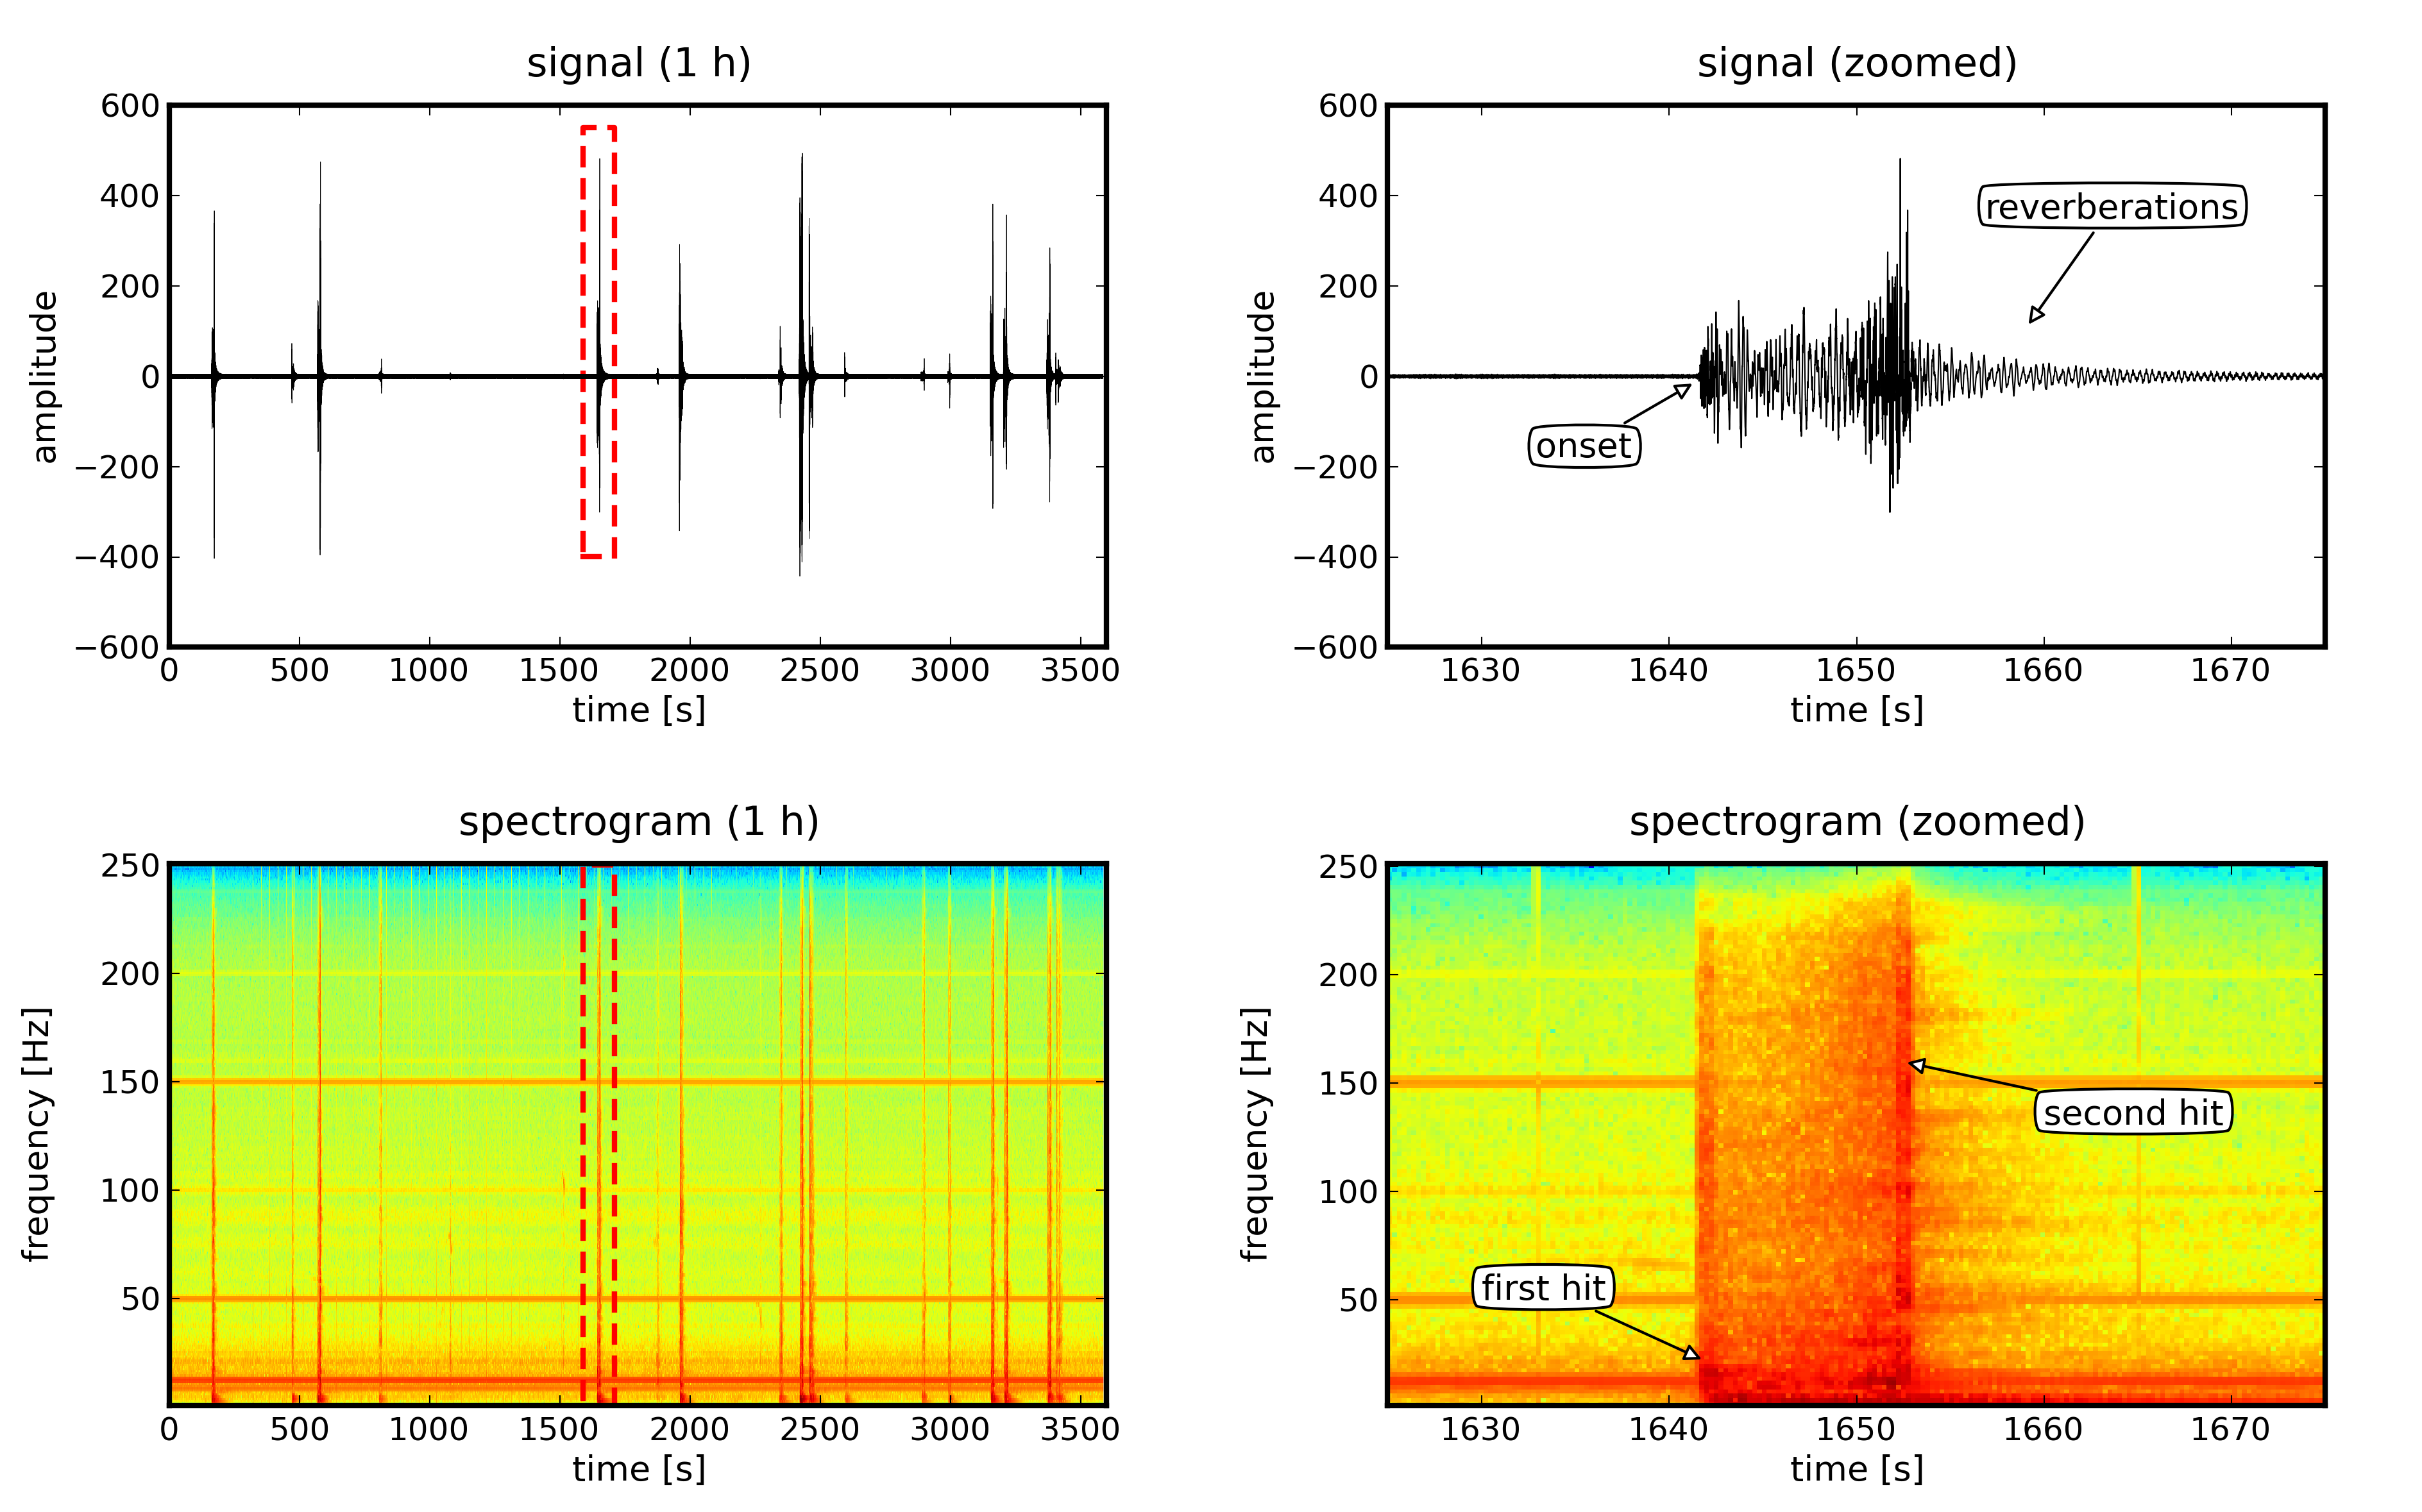
\includegraphics[width=\linewidth,height=0.89\textheight,keepaspectratio]{Figures/raw2+arrows.png}};
            \node[align=center] at (image.center) {};
            \node[anchor=center] at (image.center) {
            		\begin{tcolorbox}[colback=green!5,colframe=salve@blue,title=Spectrum (filtered), width=7cm]
						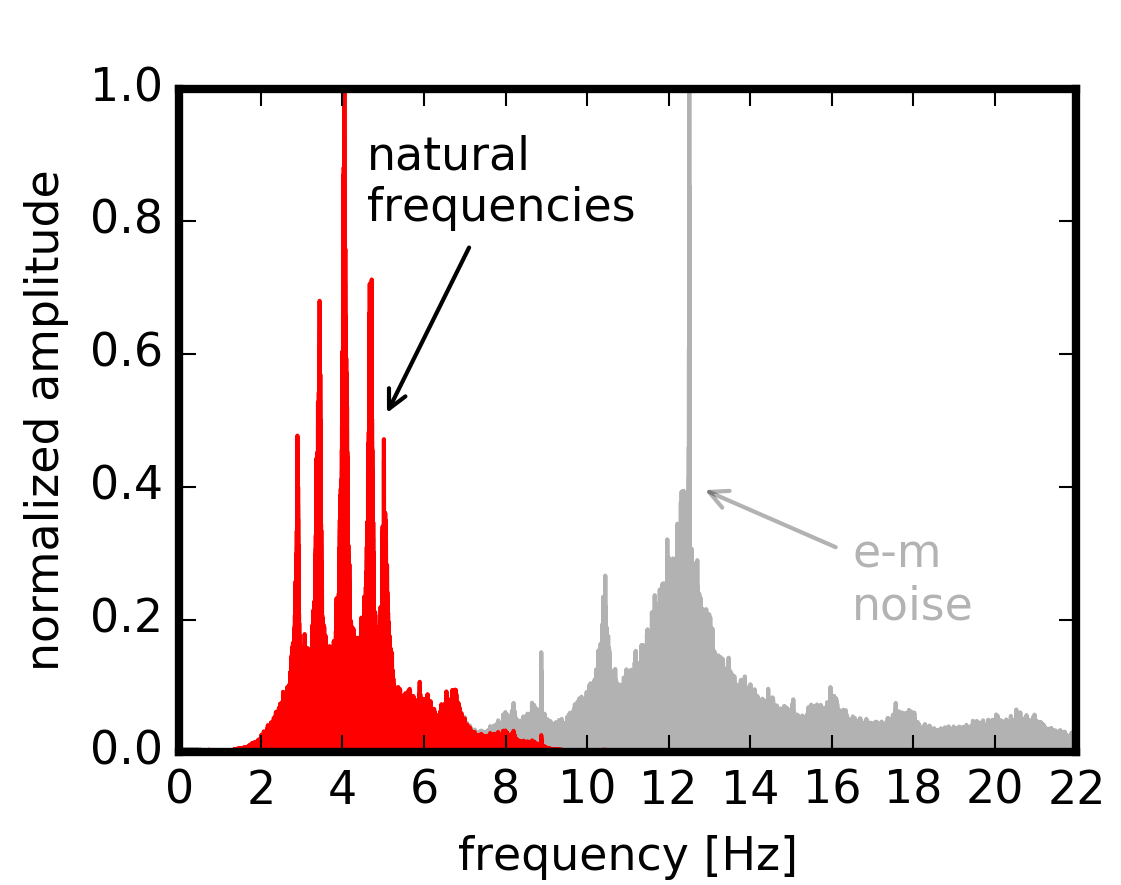
\includegraphics[width=\textwidth]{Figures/spectrum2.png}
					\end{tcolorbox}
            };
        \end{tikzpicture}
    \end{center}
\end{frame}

\begin{frame}{bla}\frametitle{Raw Signal}
	\begin{center}
        \begin{tikzpicture}
            \node[anchor=south west,inner sep=0] (image) at (0,0) 	  
            	 {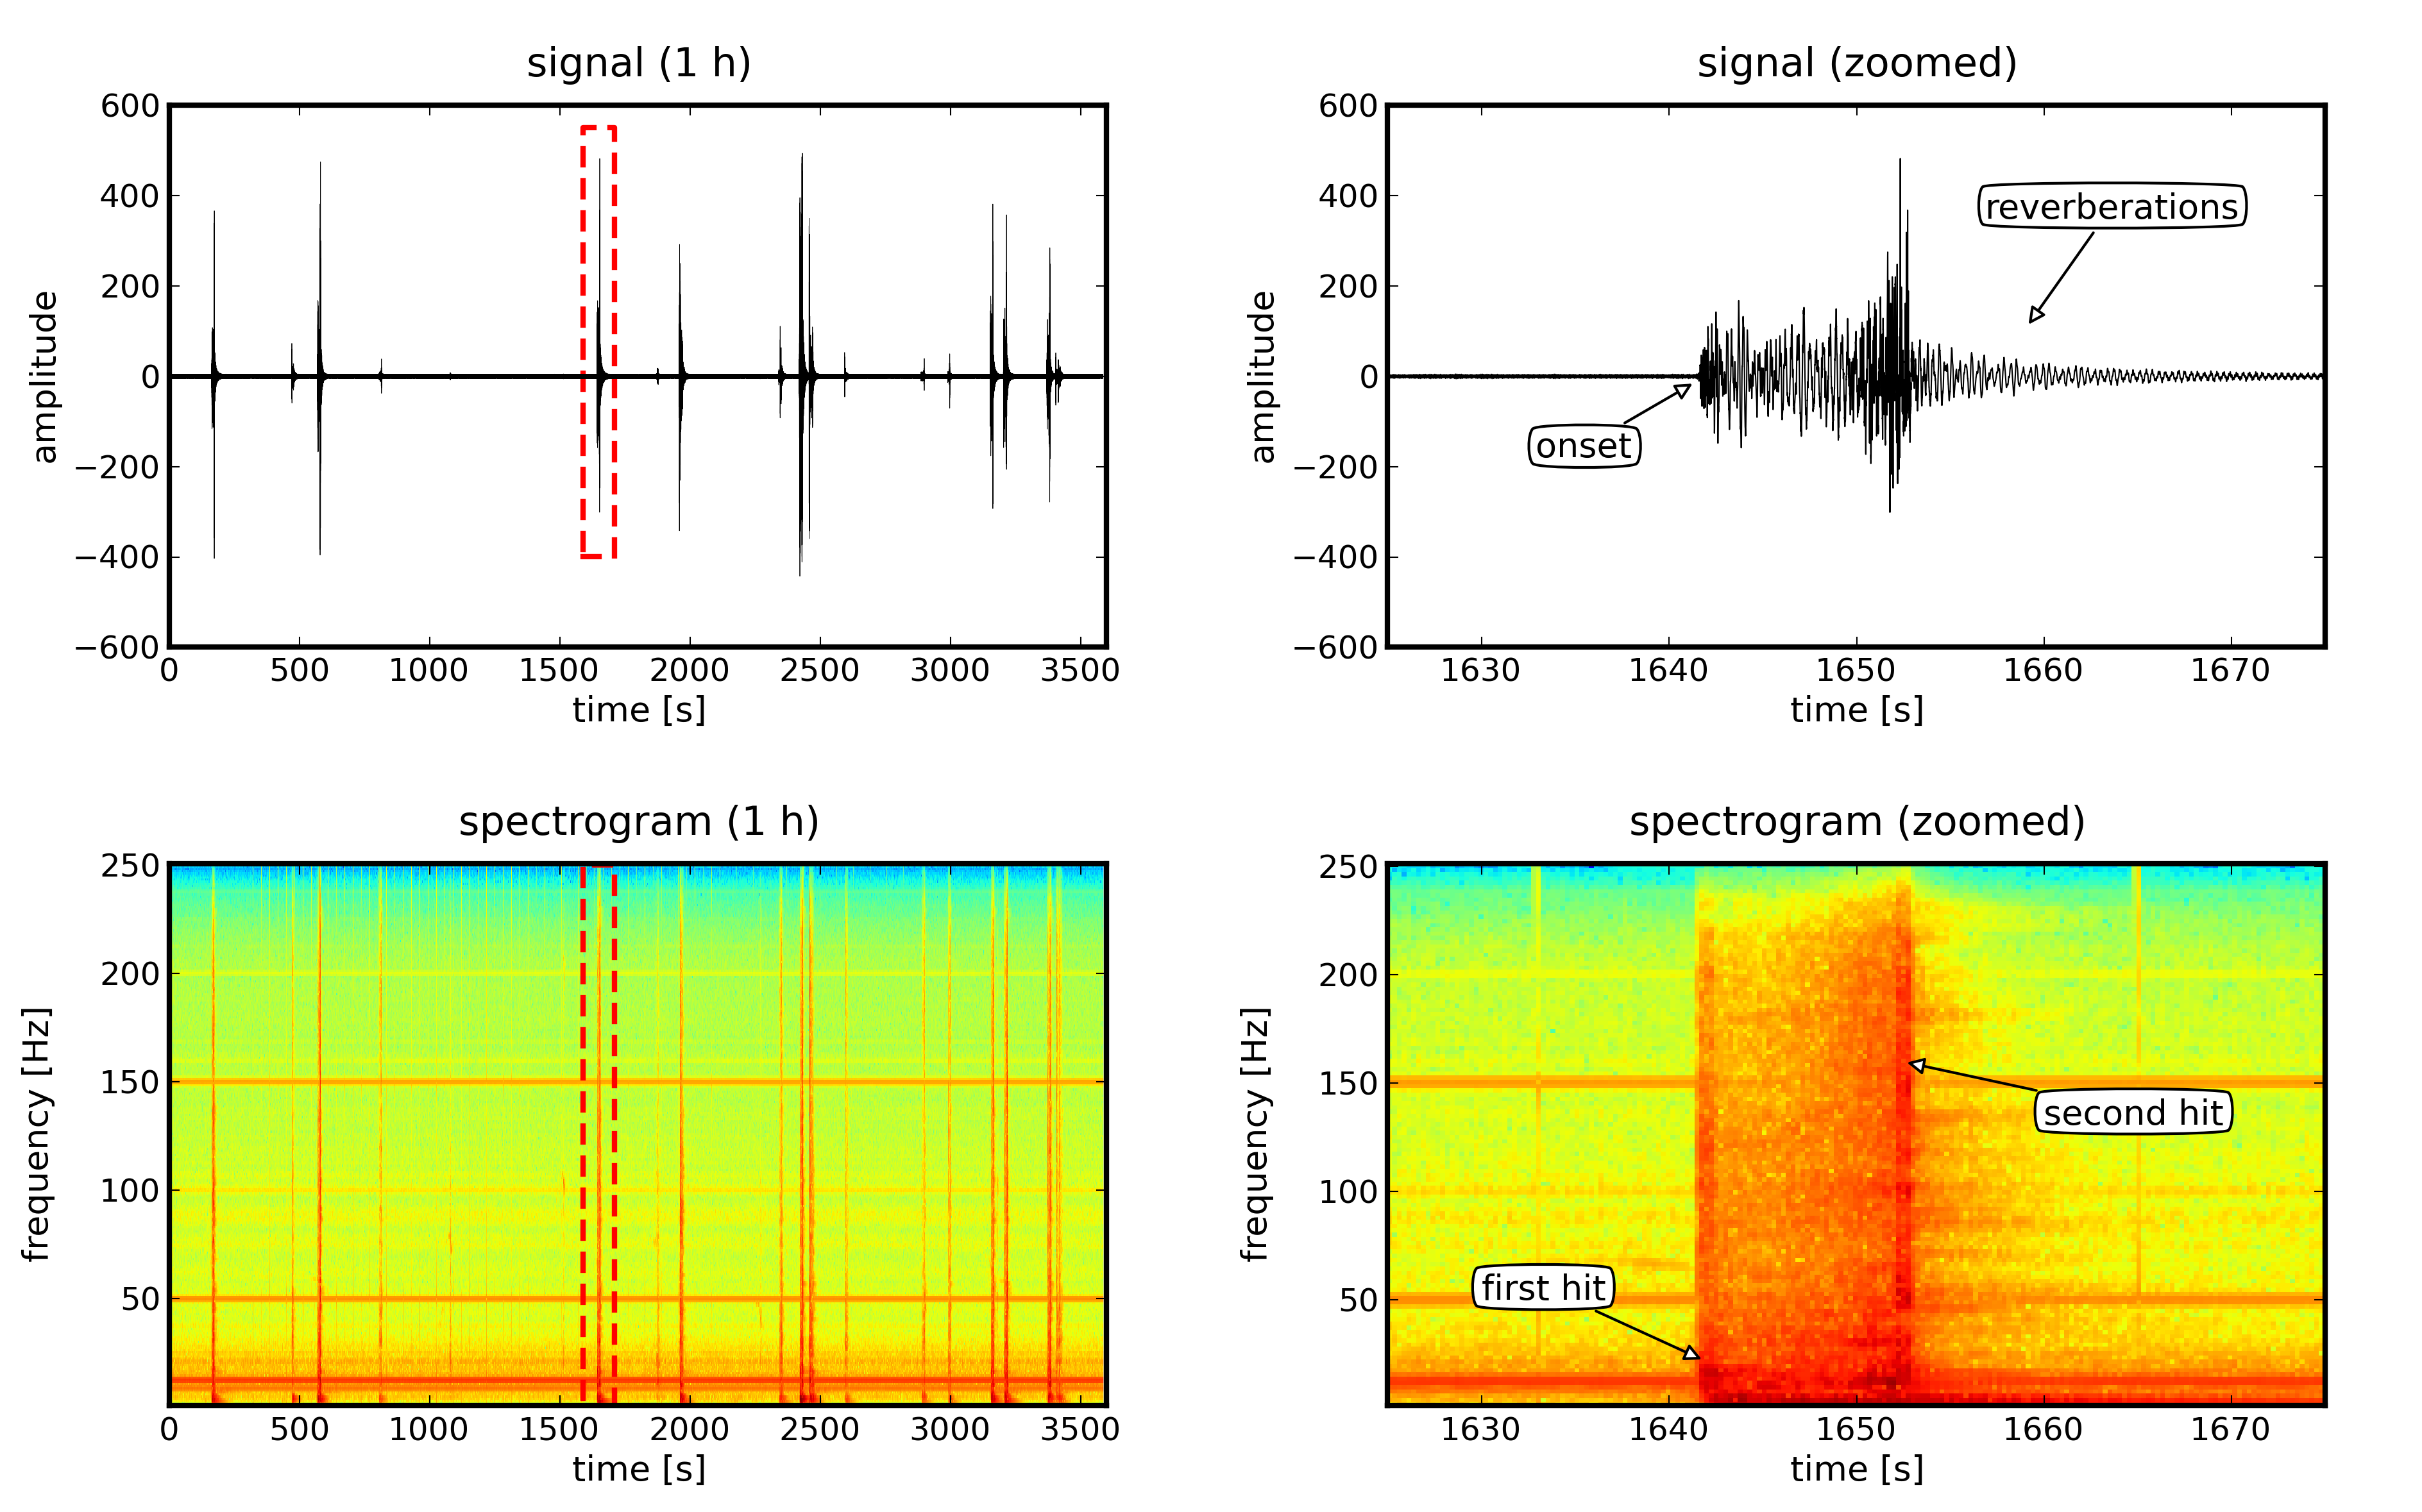
\includegraphics[width=\linewidth,height=0.89\textheight,keepaspectratio]{Figures/raw2+arrows.png}};
            \node[align=center] at (image.center) {
            \begin{small}
            		\begin{tcolorbox}[colback=green!5,colframe=salve@blue,title=Key Issues, width=7cm]
						\begin{itemize}
							\item Is it better to use the quiet parts of the signal, or those where traffic noise is present?
							\item Can we extract and resolve small velocity variations from the passive signals we observe?
							\item Can we use this information for monitoring structural health?
							\end{itemize}
					\end{tcolorbox}
            	\end{small}
            	};
        \end{tikzpicture}
    \end{center}
\end{frame}


\section{Method}
\subsection{Stretching}
\begin{frame}{bla}\frametitle{CWI \& Cross-correlations}
	\begin{center}
        \begin{tikzpicture}
            \node[anchor=south west,inner sep=0] (image) at (0,0) 	  
            	 {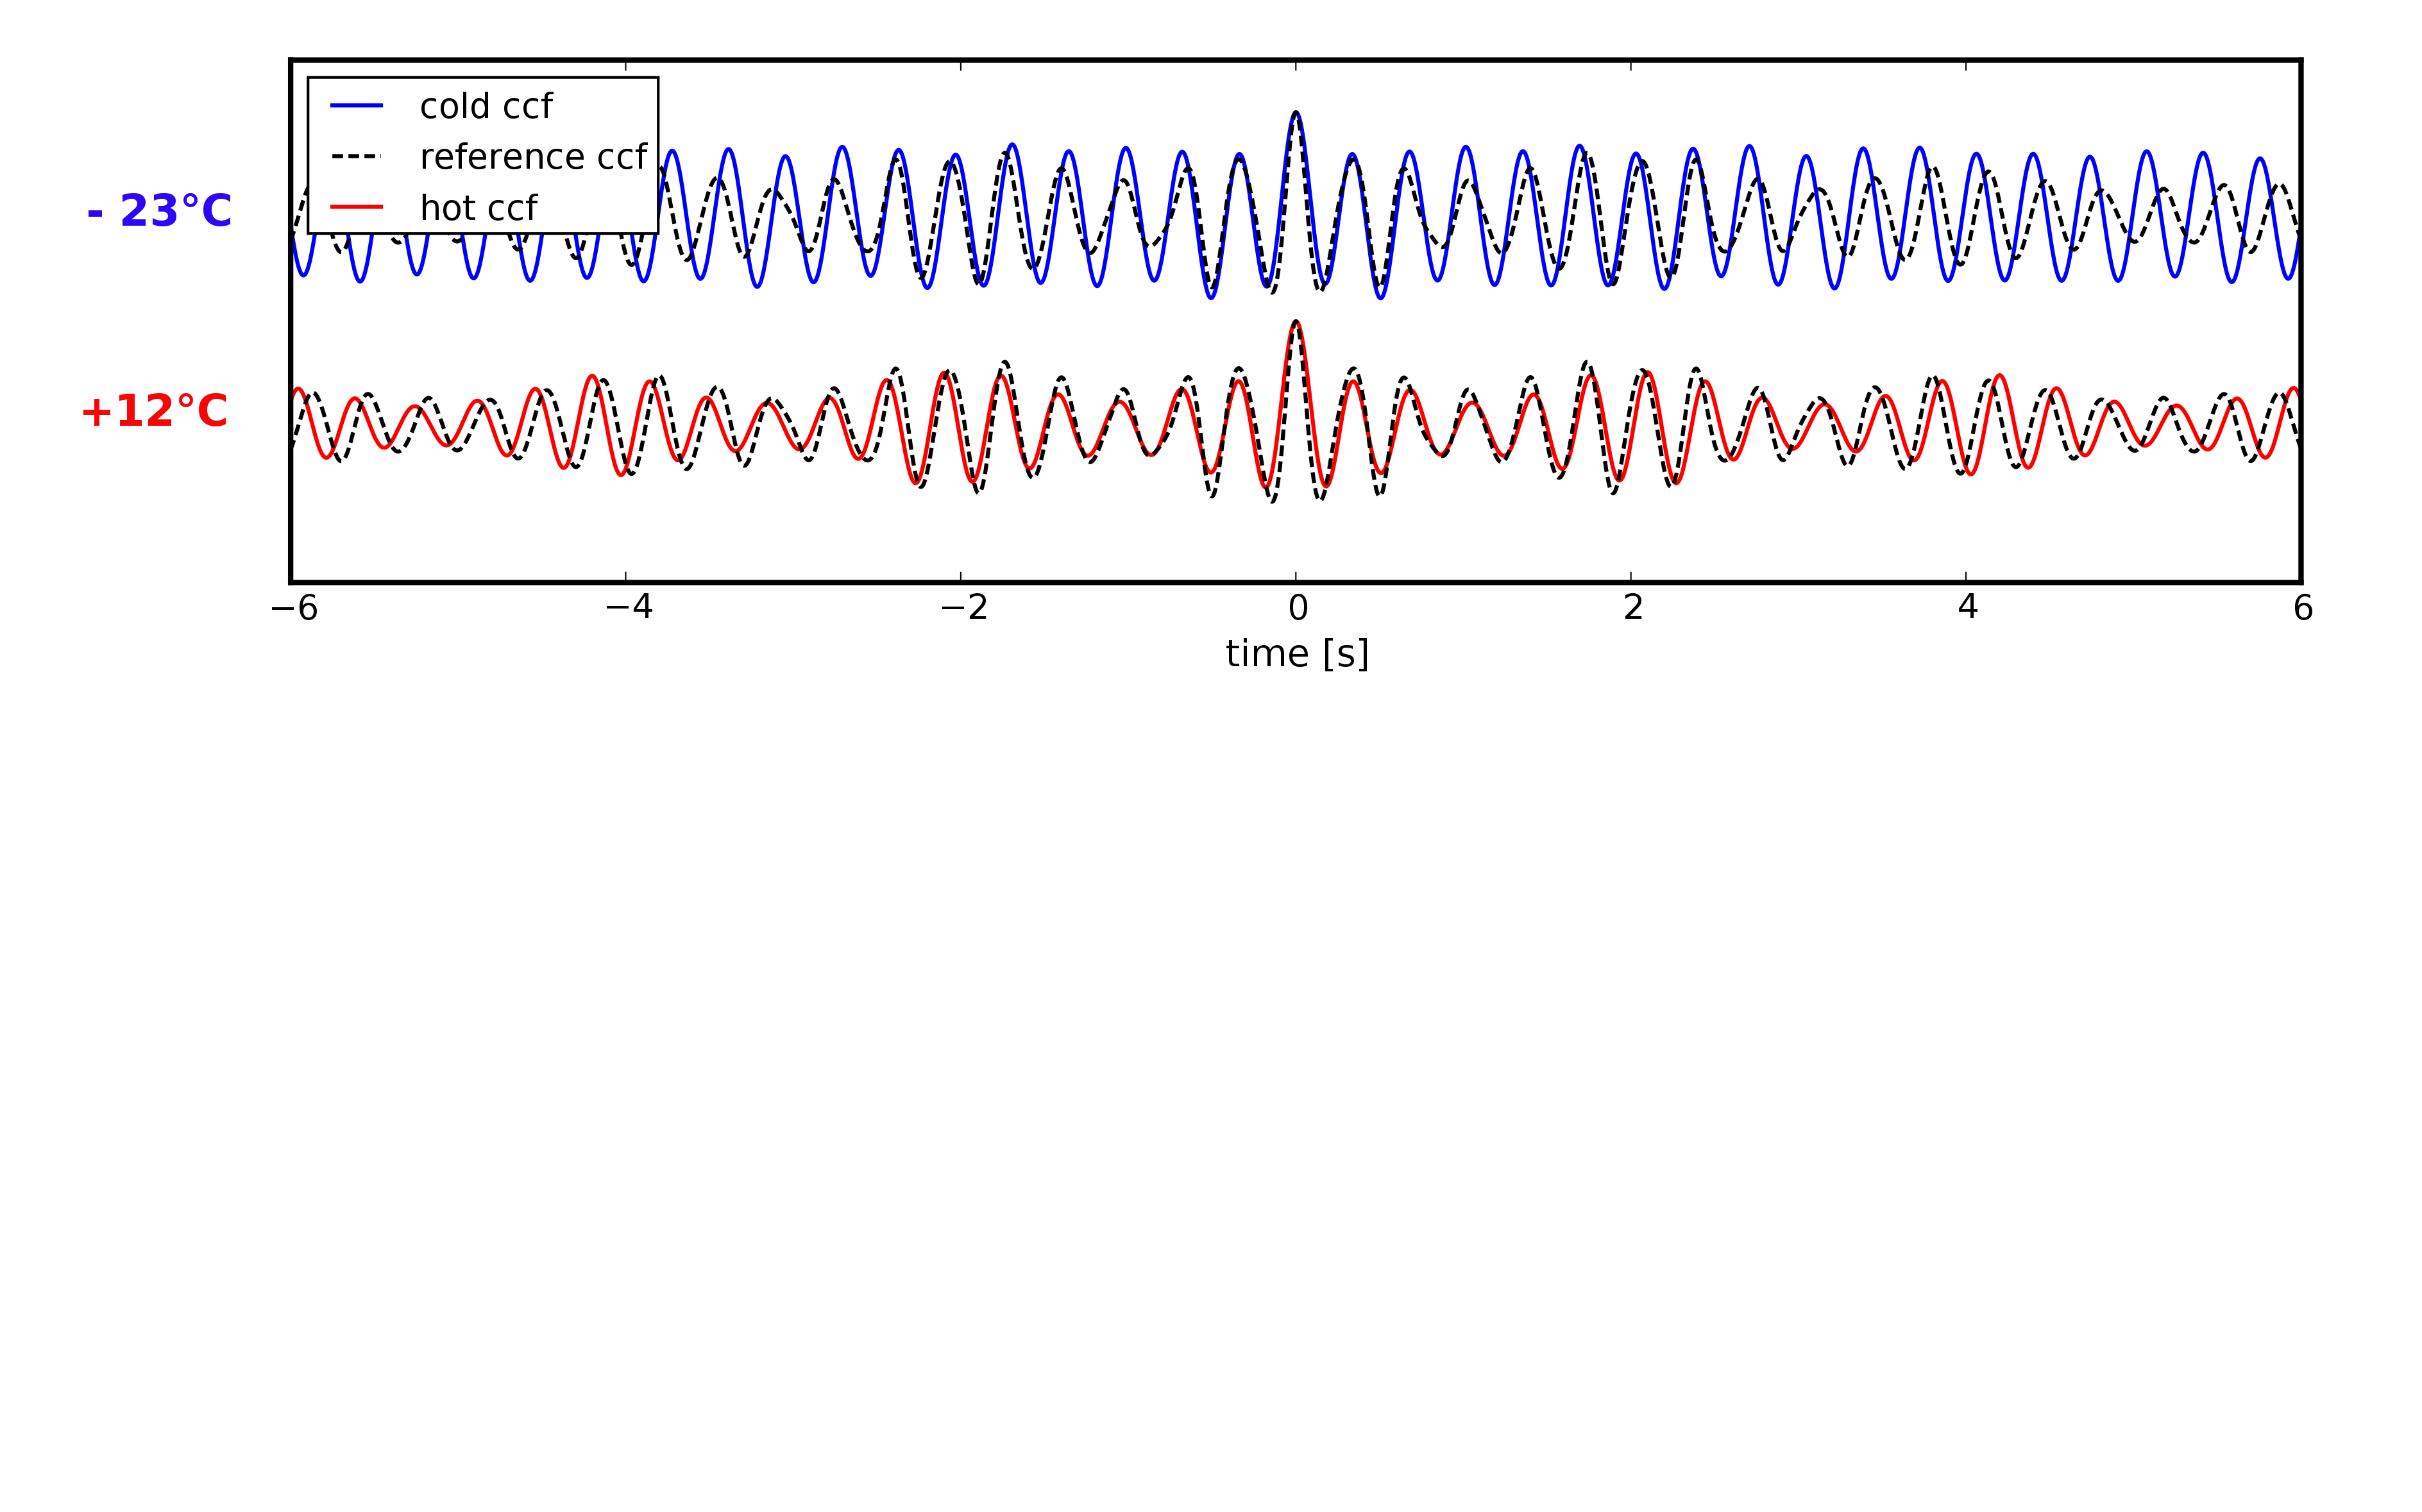
\includegraphics[width=\linewidth,height=0.89\textheight,keepaspectratio]{Figures/hot_cold1.png}};
        \end{tikzpicture}
    \end{center}
\end{frame}

\begin{frame}{bla}\frametitle{CWI \& Cross-correlations}
	\begin{center}
        \begin{tikzpicture}
            \node[anchor=south west,inner sep=0] (image) at (0,0) 	  
            	 {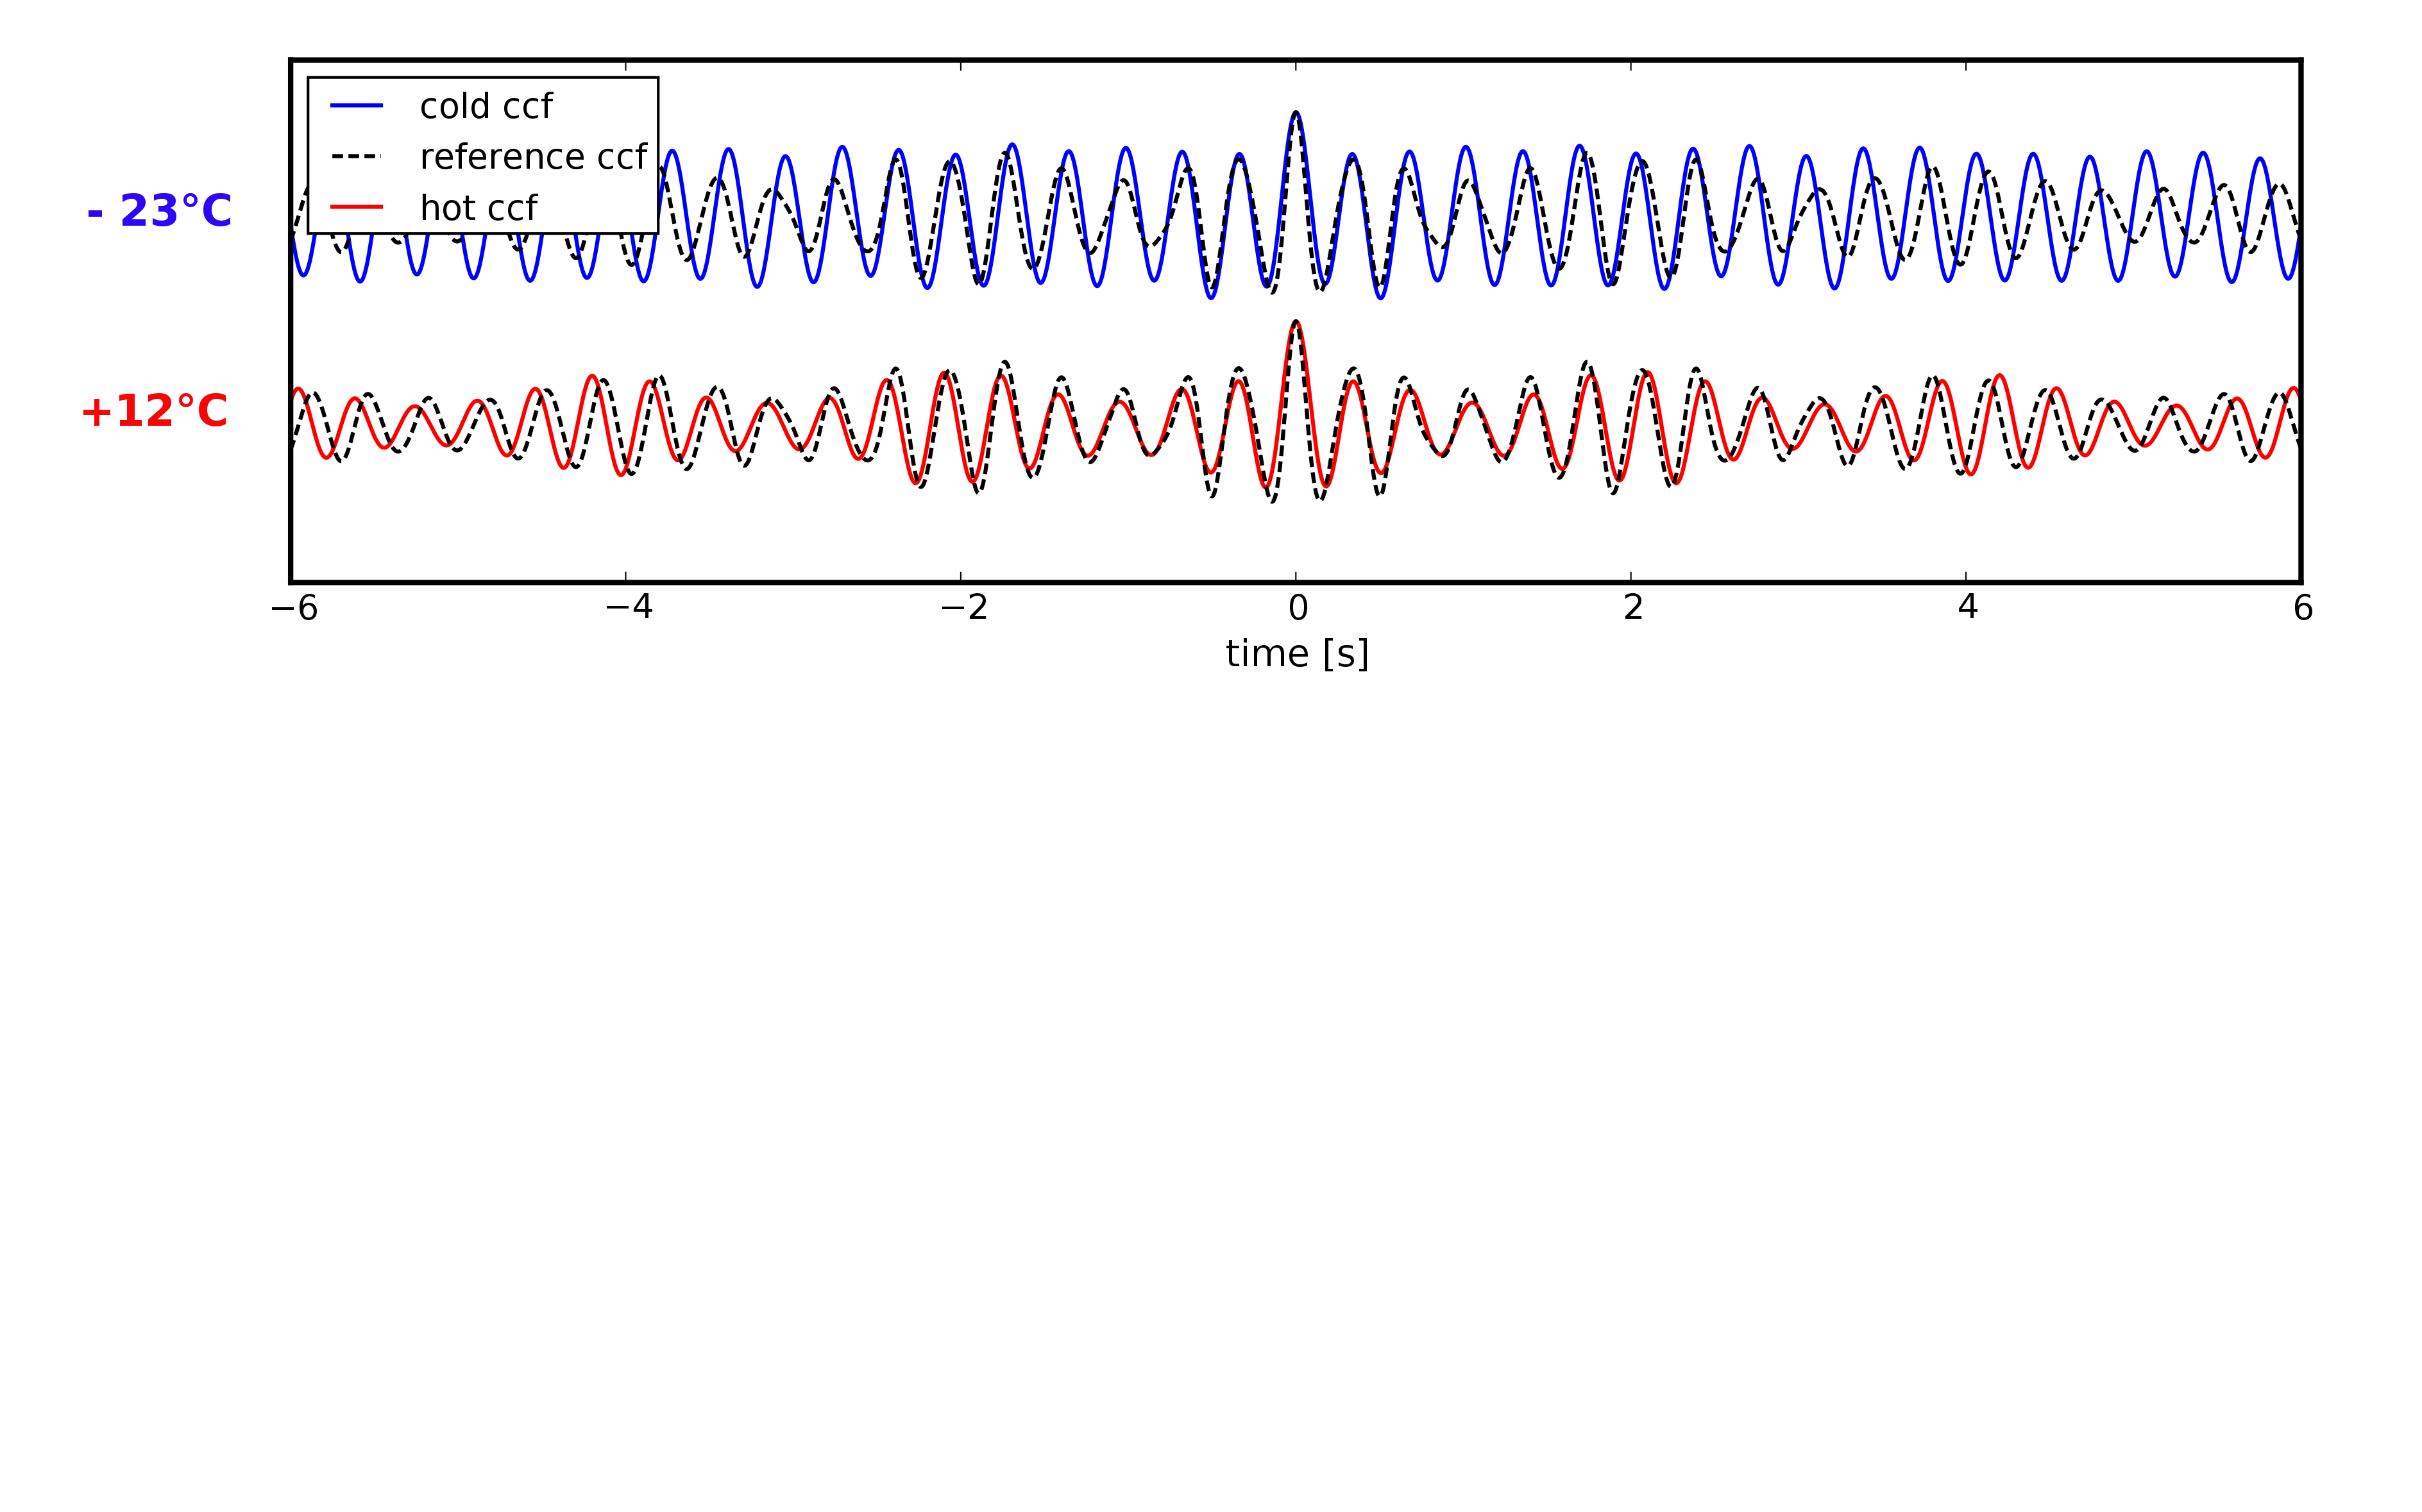
\includegraphics[width=\linewidth,height=0.89\textheight,keepaspectratio]{Figures/hot_cold1.png}};
            \node[anchor=south west,inner sep=0] at (1.3,0.6)
            	 {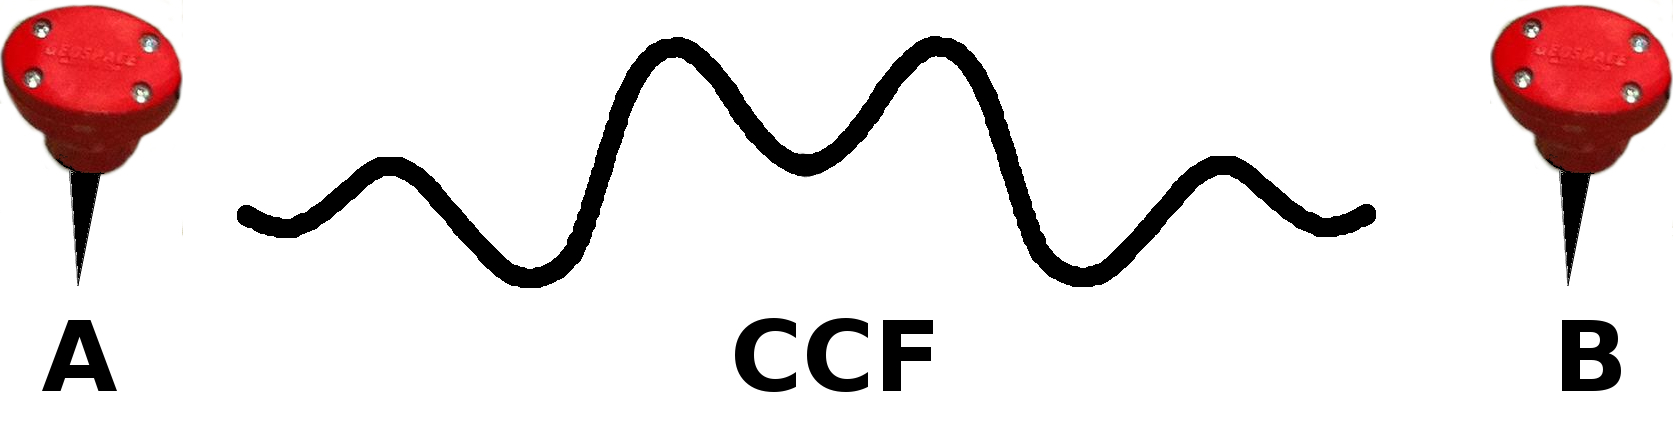
\includegraphics[width=0.4\linewidth]{Figures/cc.JPG}};  
            \node[anchor=south west,inner sep=0] at (1,2.2) {
            	\begin{small}
            		\begin{tcolorbox}[colback=green!5,colframe=salve@blue,title=, width=5cm]
						\textbf{Hourly} cross-correlations for receiver pairs
					\end{tcolorbox}
            	\end{small}
            };
            \node[anchor=south west,inner sep=0] at (6.8,1) {
            	\begin{small}
            		\begin{tcolorbox}[colback=green!5,colframe=salve@blue,title=, width=4cm]
						\textbf{Unilateral} sources and reverberations \begin{center} $\Downarrow$ \end{center}
						\textbf{No} Green's function retrieval
					\end{tcolorbox}
            	\end{small}
            };        
        \end{tikzpicture}
    \end{center}
\end{frame}

\begin{frame}{bla}\frametitle{CWI \& Cross-correlations}
	\begin{center}
        \begin{tikzpicture}
            \node[anchor=south west,inner sep=0] (image) at (0,0) 	  
            	 {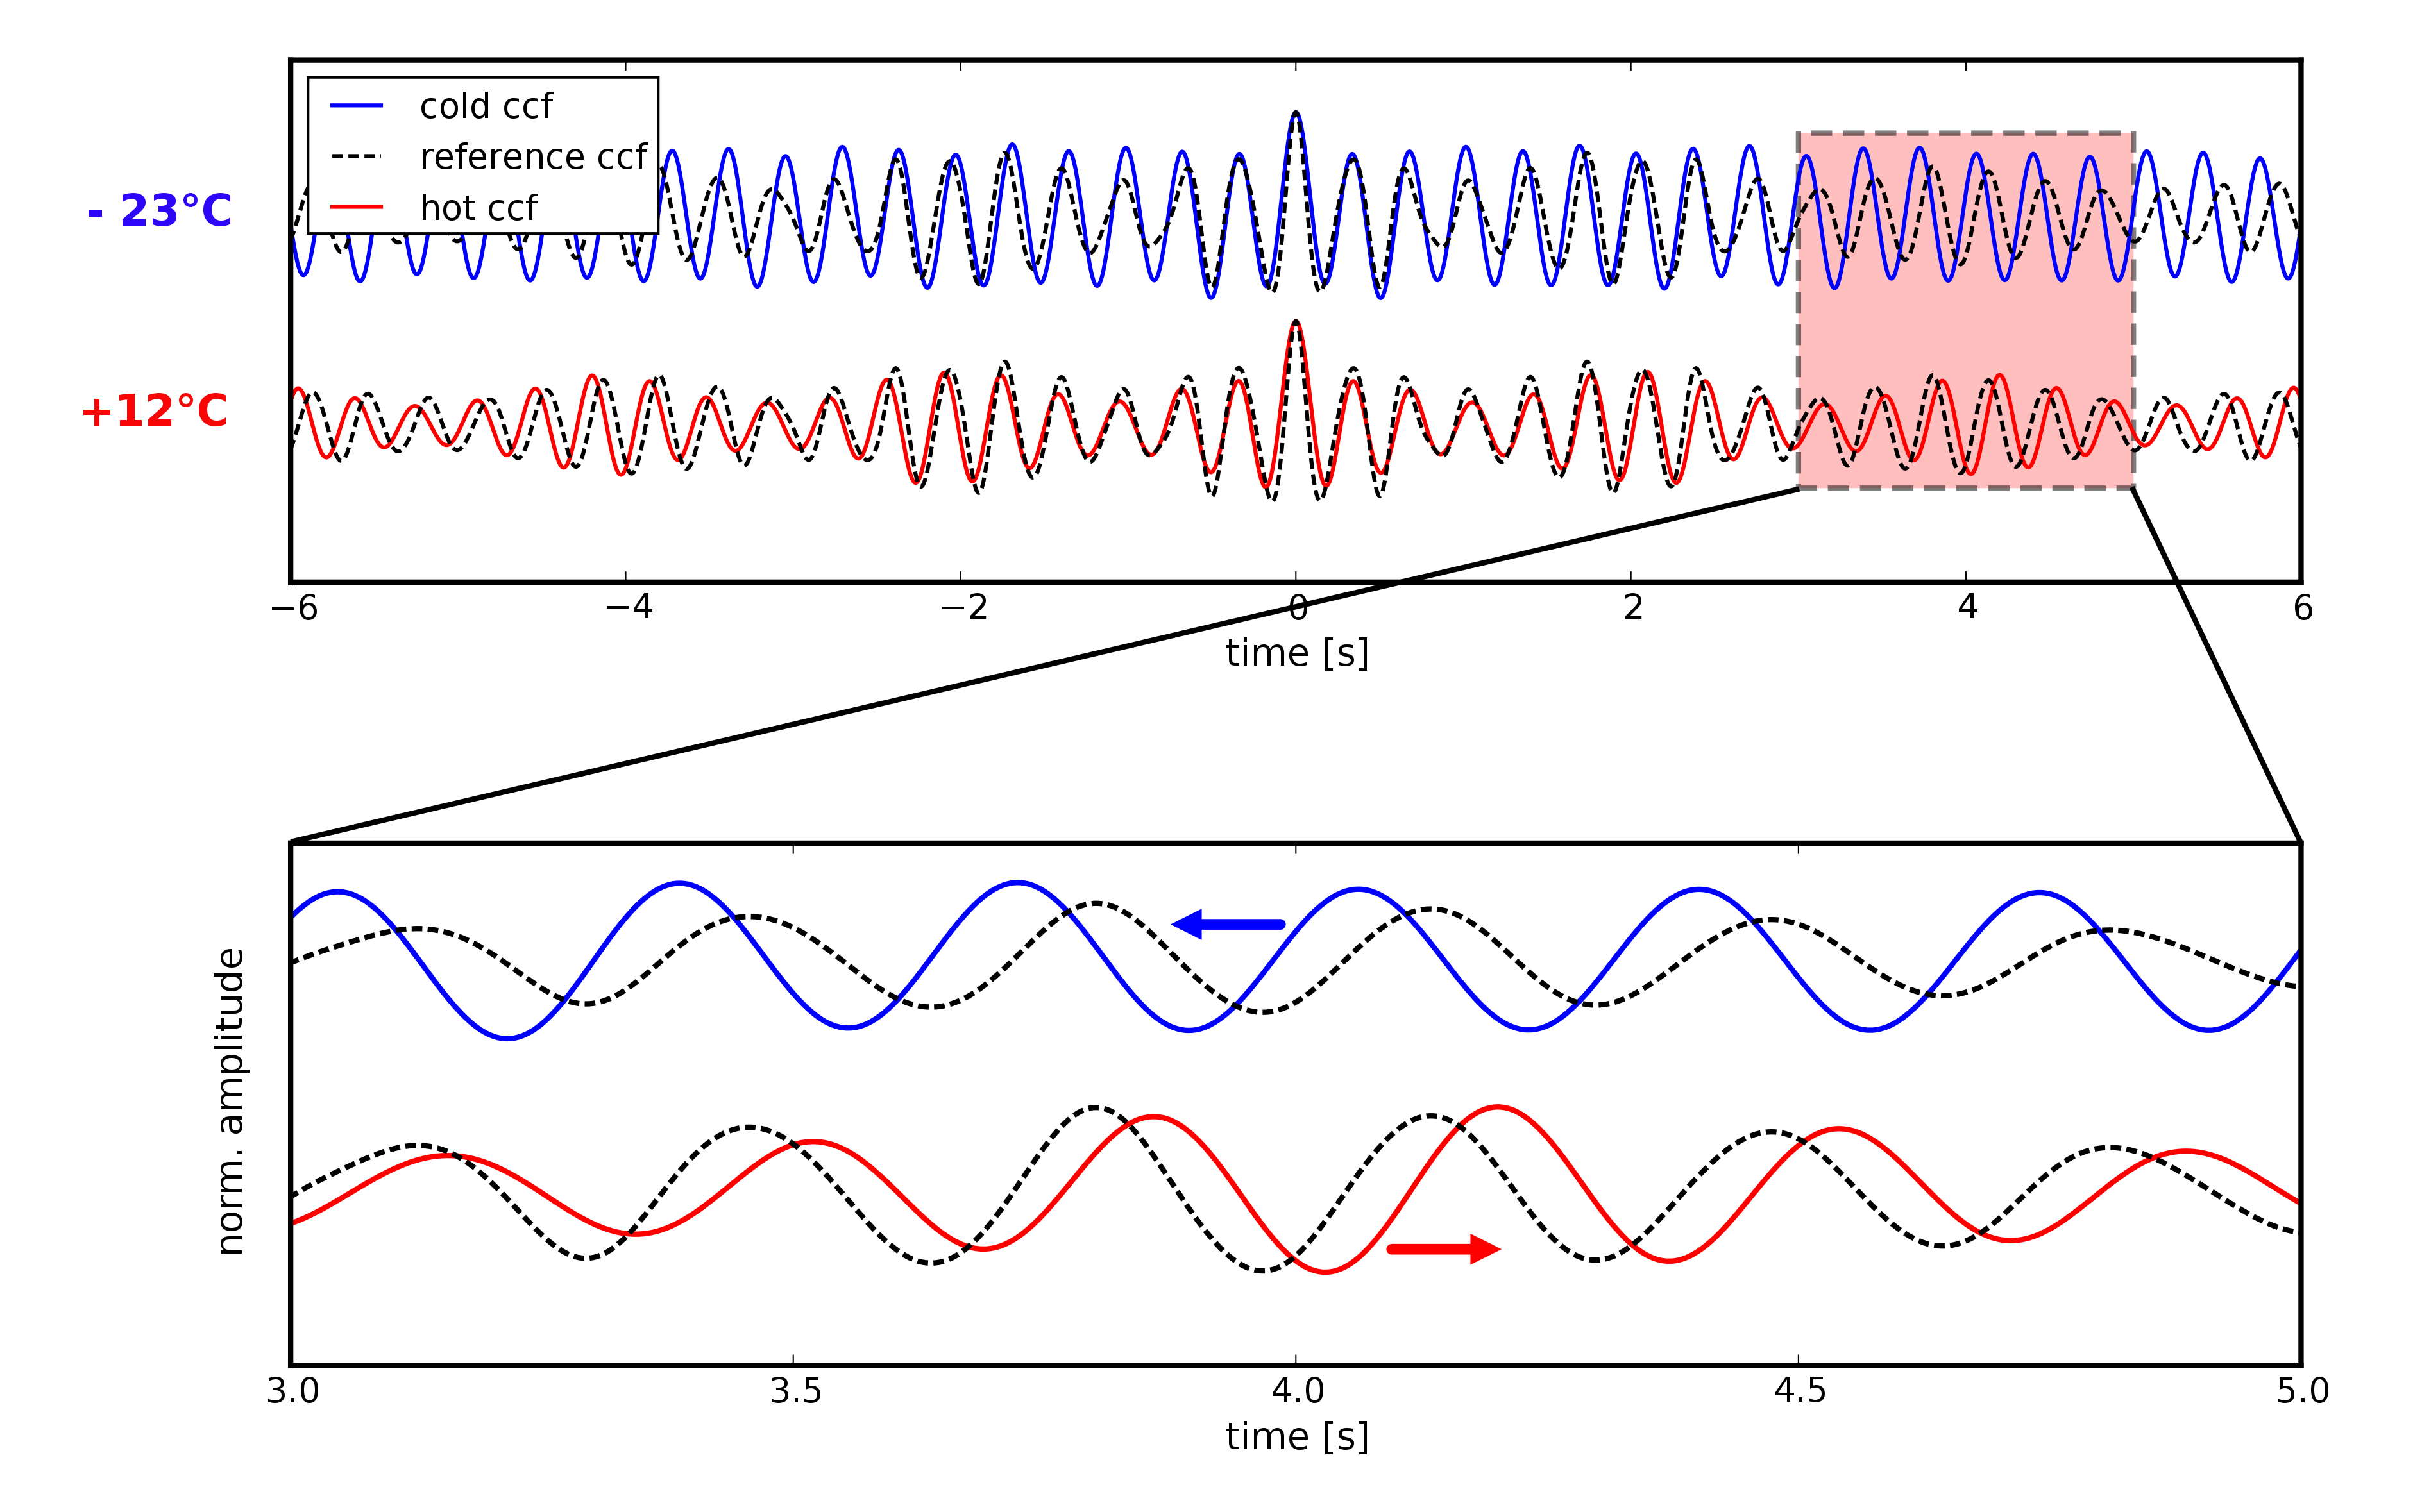
\includegraphics[width=\linewidth,height=0.89\textheight,keepaspectratio]{Figures/hot_cold3.png}};
            \node[align=center] at (image.center) {};
        \end{tikzpicture}
    \end{center}
\end{frame}

\begin{frame}{bla}\frametitle{CWI \& Cross-correlations}
	\begin{center}
        \begin{tikzpicture}
            \node[anchor=south west,inner sep=0] (image) at (0,0) 	  
            	 {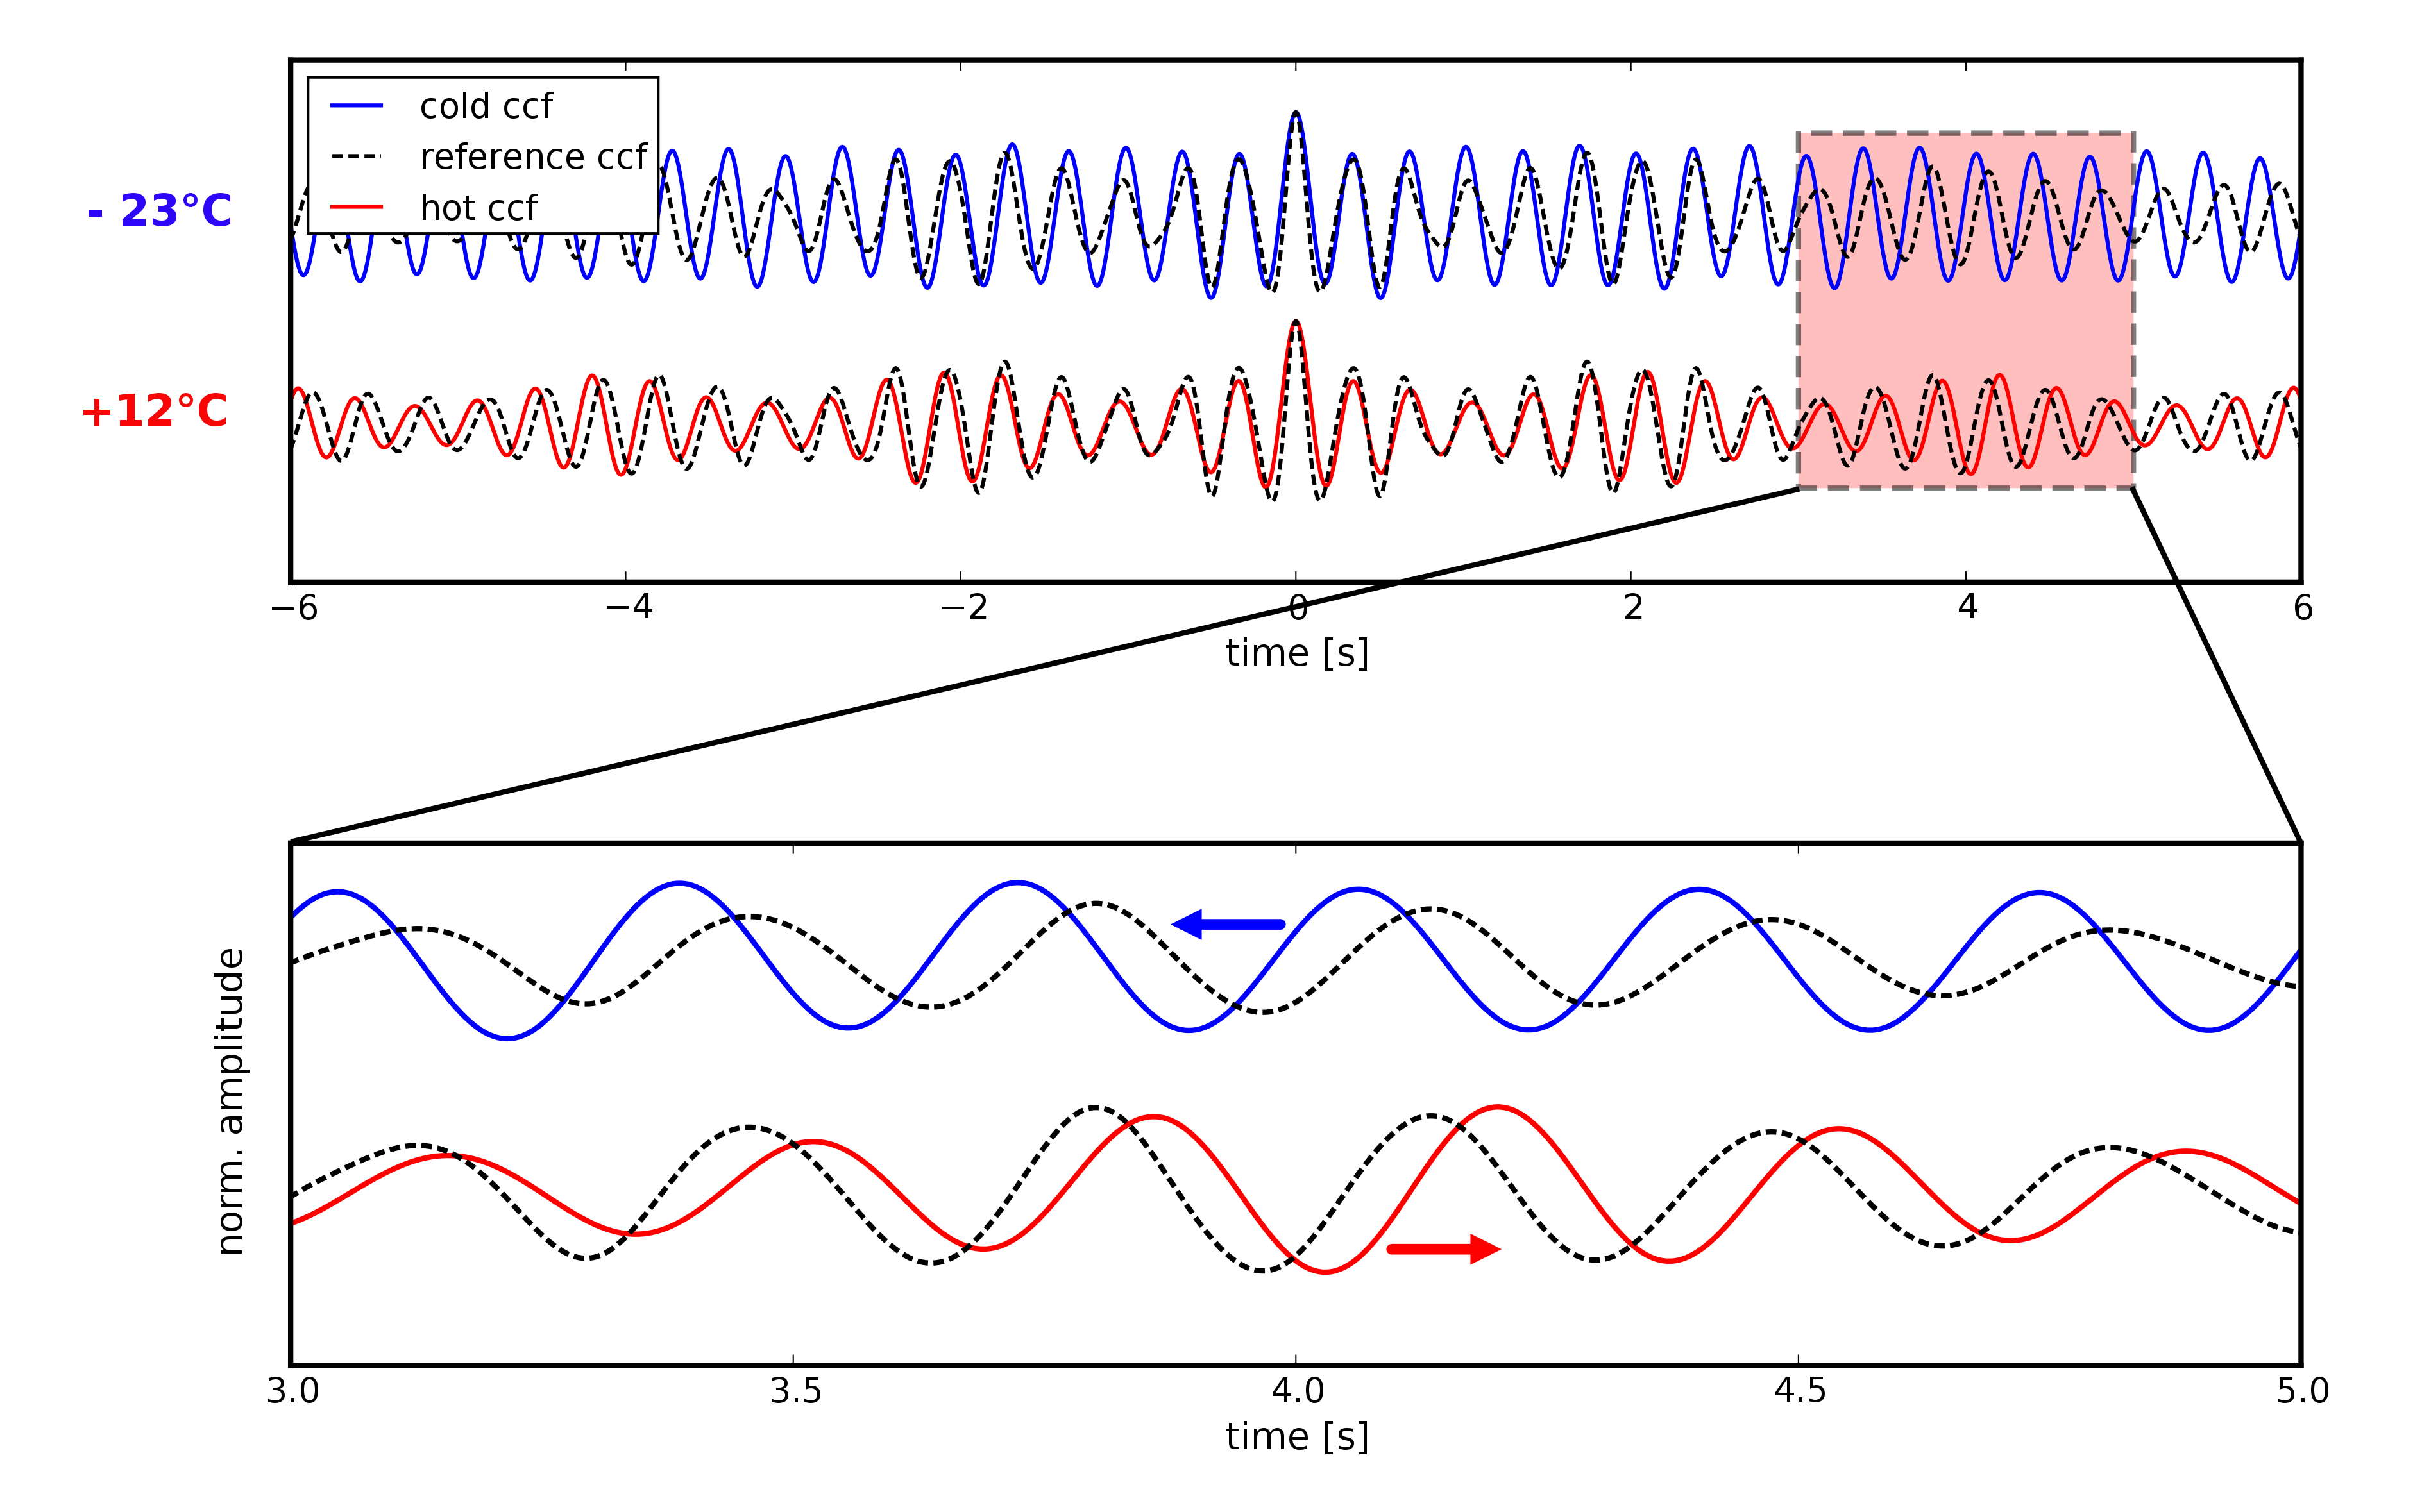
\includegraphics[width=\linewidth,height=0.89\textheight,keepaspectratio]{Figures/hot_cold3.png}};
            \node[anchor=center] (statements) at (image.center) {
            	\begin{small}
            		\begin{tcolorbox}[colback=green!5,colframe=salve@blue,title=Statements, width=8cm]
						\begin{itemize}
							\item Traffic noise is required for sufficiently high SNR
							\item Reverberations for natural frequencies around 3 Hz last long enough and can be used for CWI 
							\item Stretching was used to quantify wavespeed changes
							\item Analysis applied to two months of contiunous recordings
						\end{itemize}
					\end{tcolorbox}
            	\end{small}
            };        
        \end{tikzpicture}
    \end{center}
\end{frame}

% =============================================================================
\section{Results}
\subsection{Results}
\begin{frame}{bla}\frametitle{Observed Results}
	\begin{center}
        \begin{tikzpicture}[overlay]
            \node[anchor=south west,inner sep=0] (image) at (-6,-3.4) {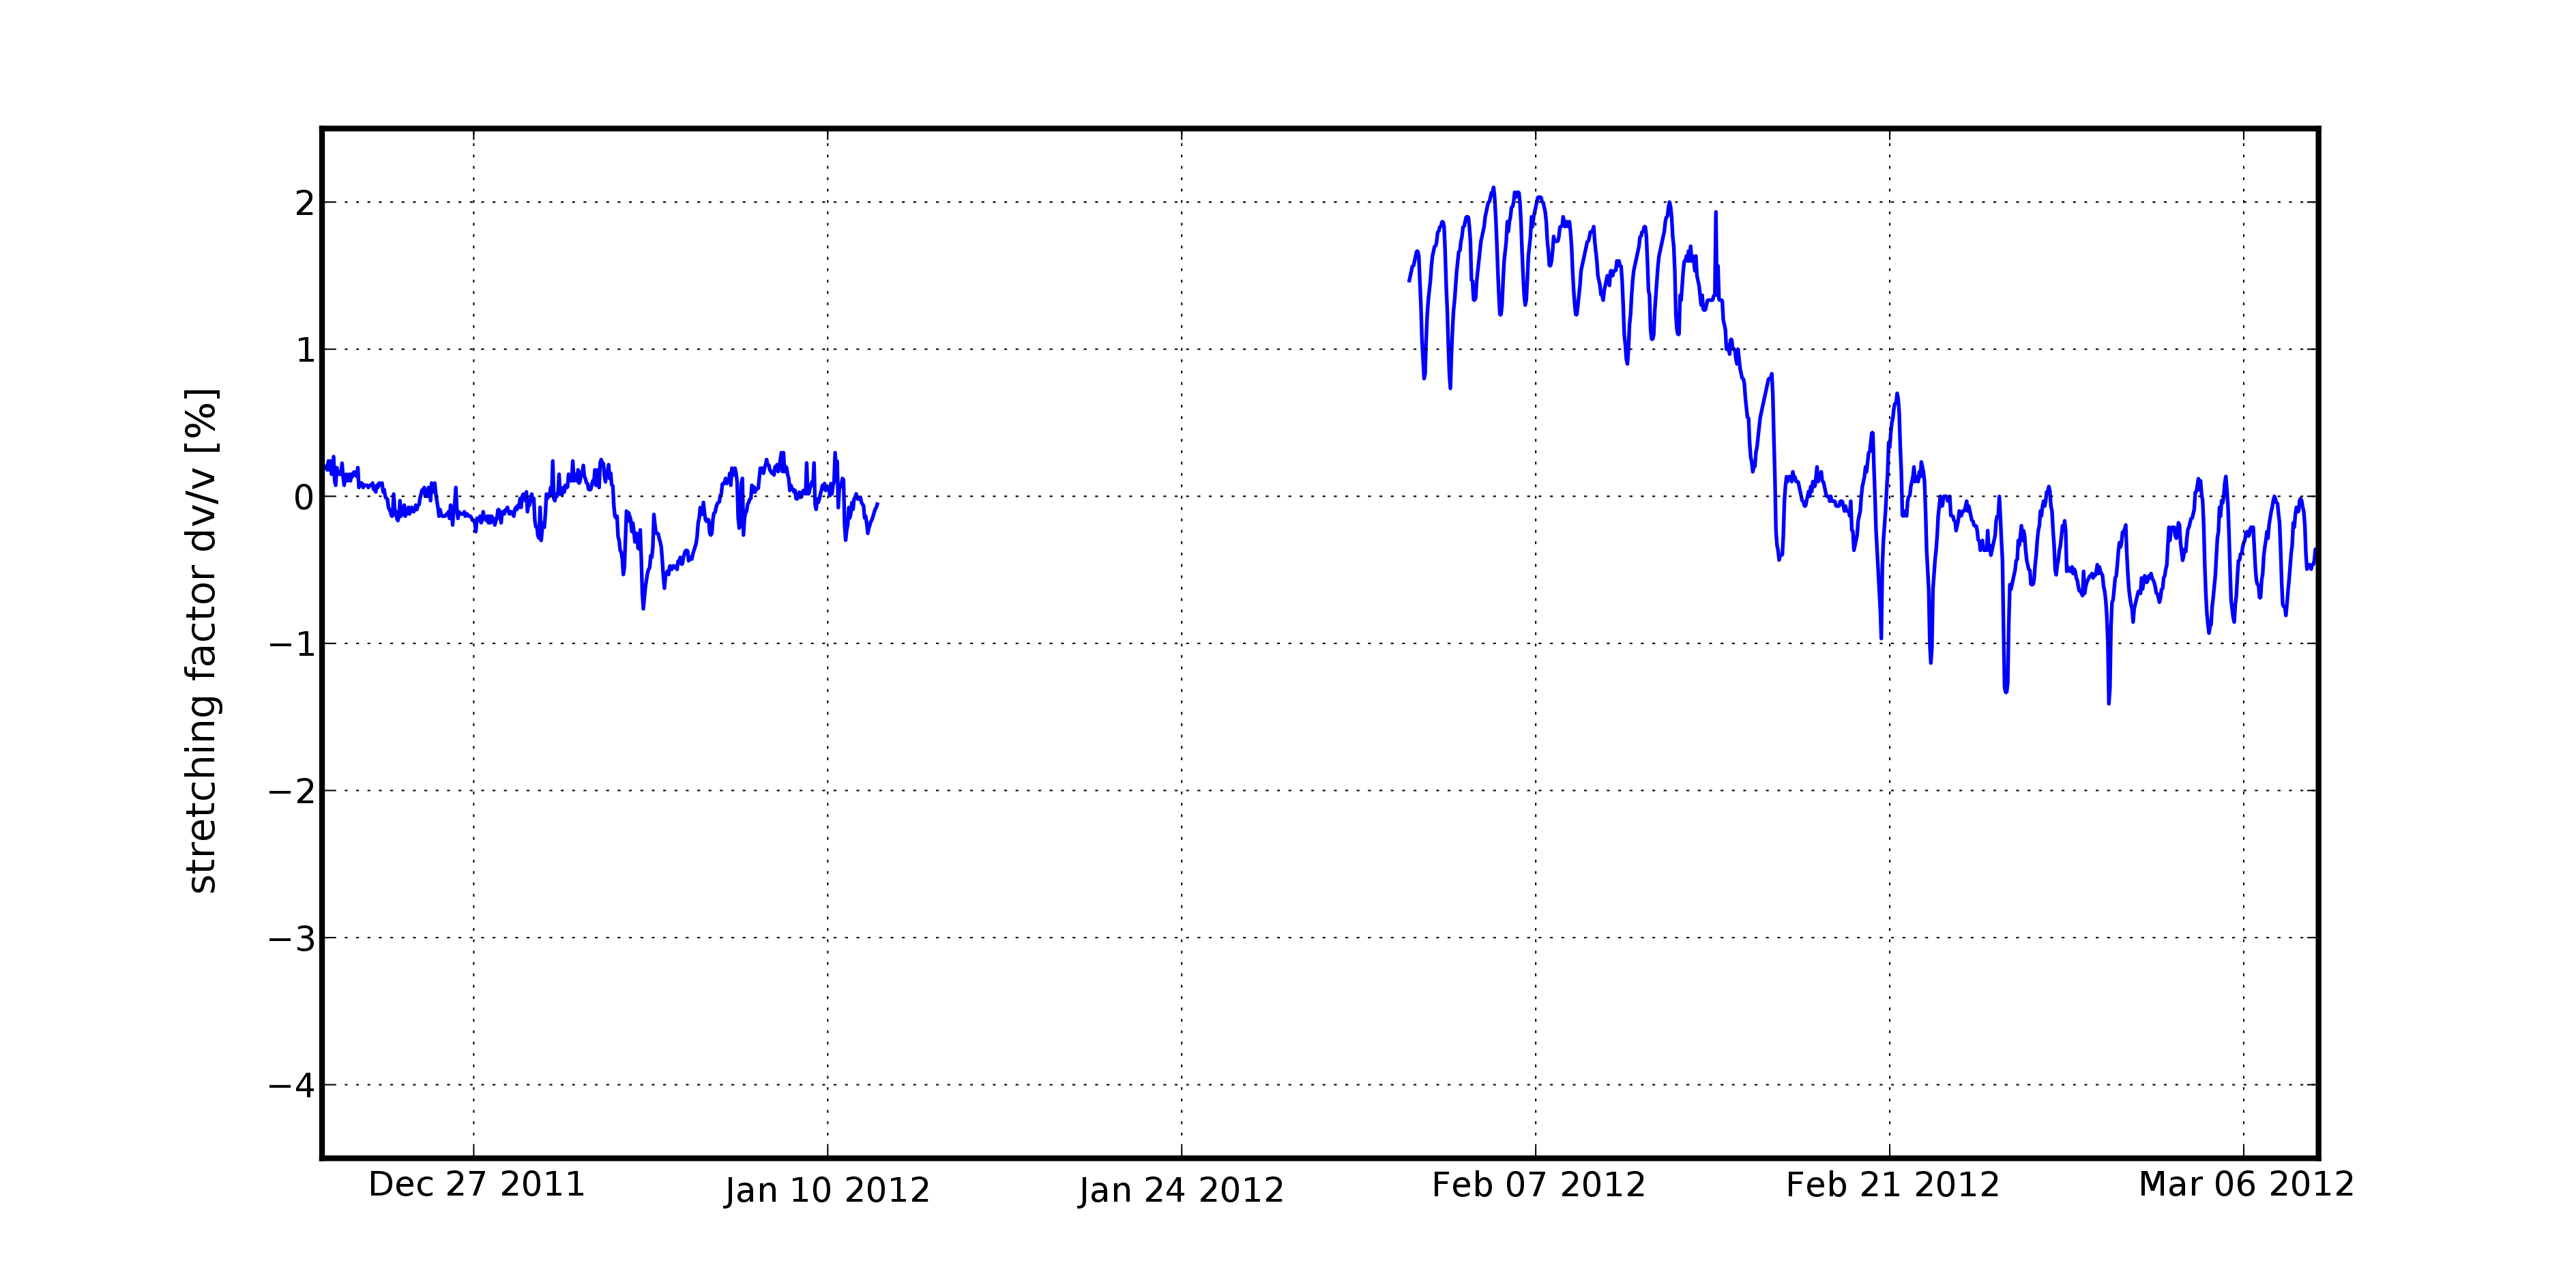
\includegraphics[width=\linewidth,height=0.89\textheight,keepaspectratio]{Figures/whole1_flip.png}};
			 \node[anchor=south west,inner sep=0] at (-4.5,2.5) {\textbf{\color{blue} Velocity variation $\frac{\Delta v}{v}$}};
        \end{tikzpicture}
    \end{center}
\end{frame}

\begin{frame}{bla}\frametitle{Observed Results}
	\begin{center}
        \begin{tikzpicture}[overlay]
            \node[anchor=south west,inner sep=0] (image) at (-6,-3.4) {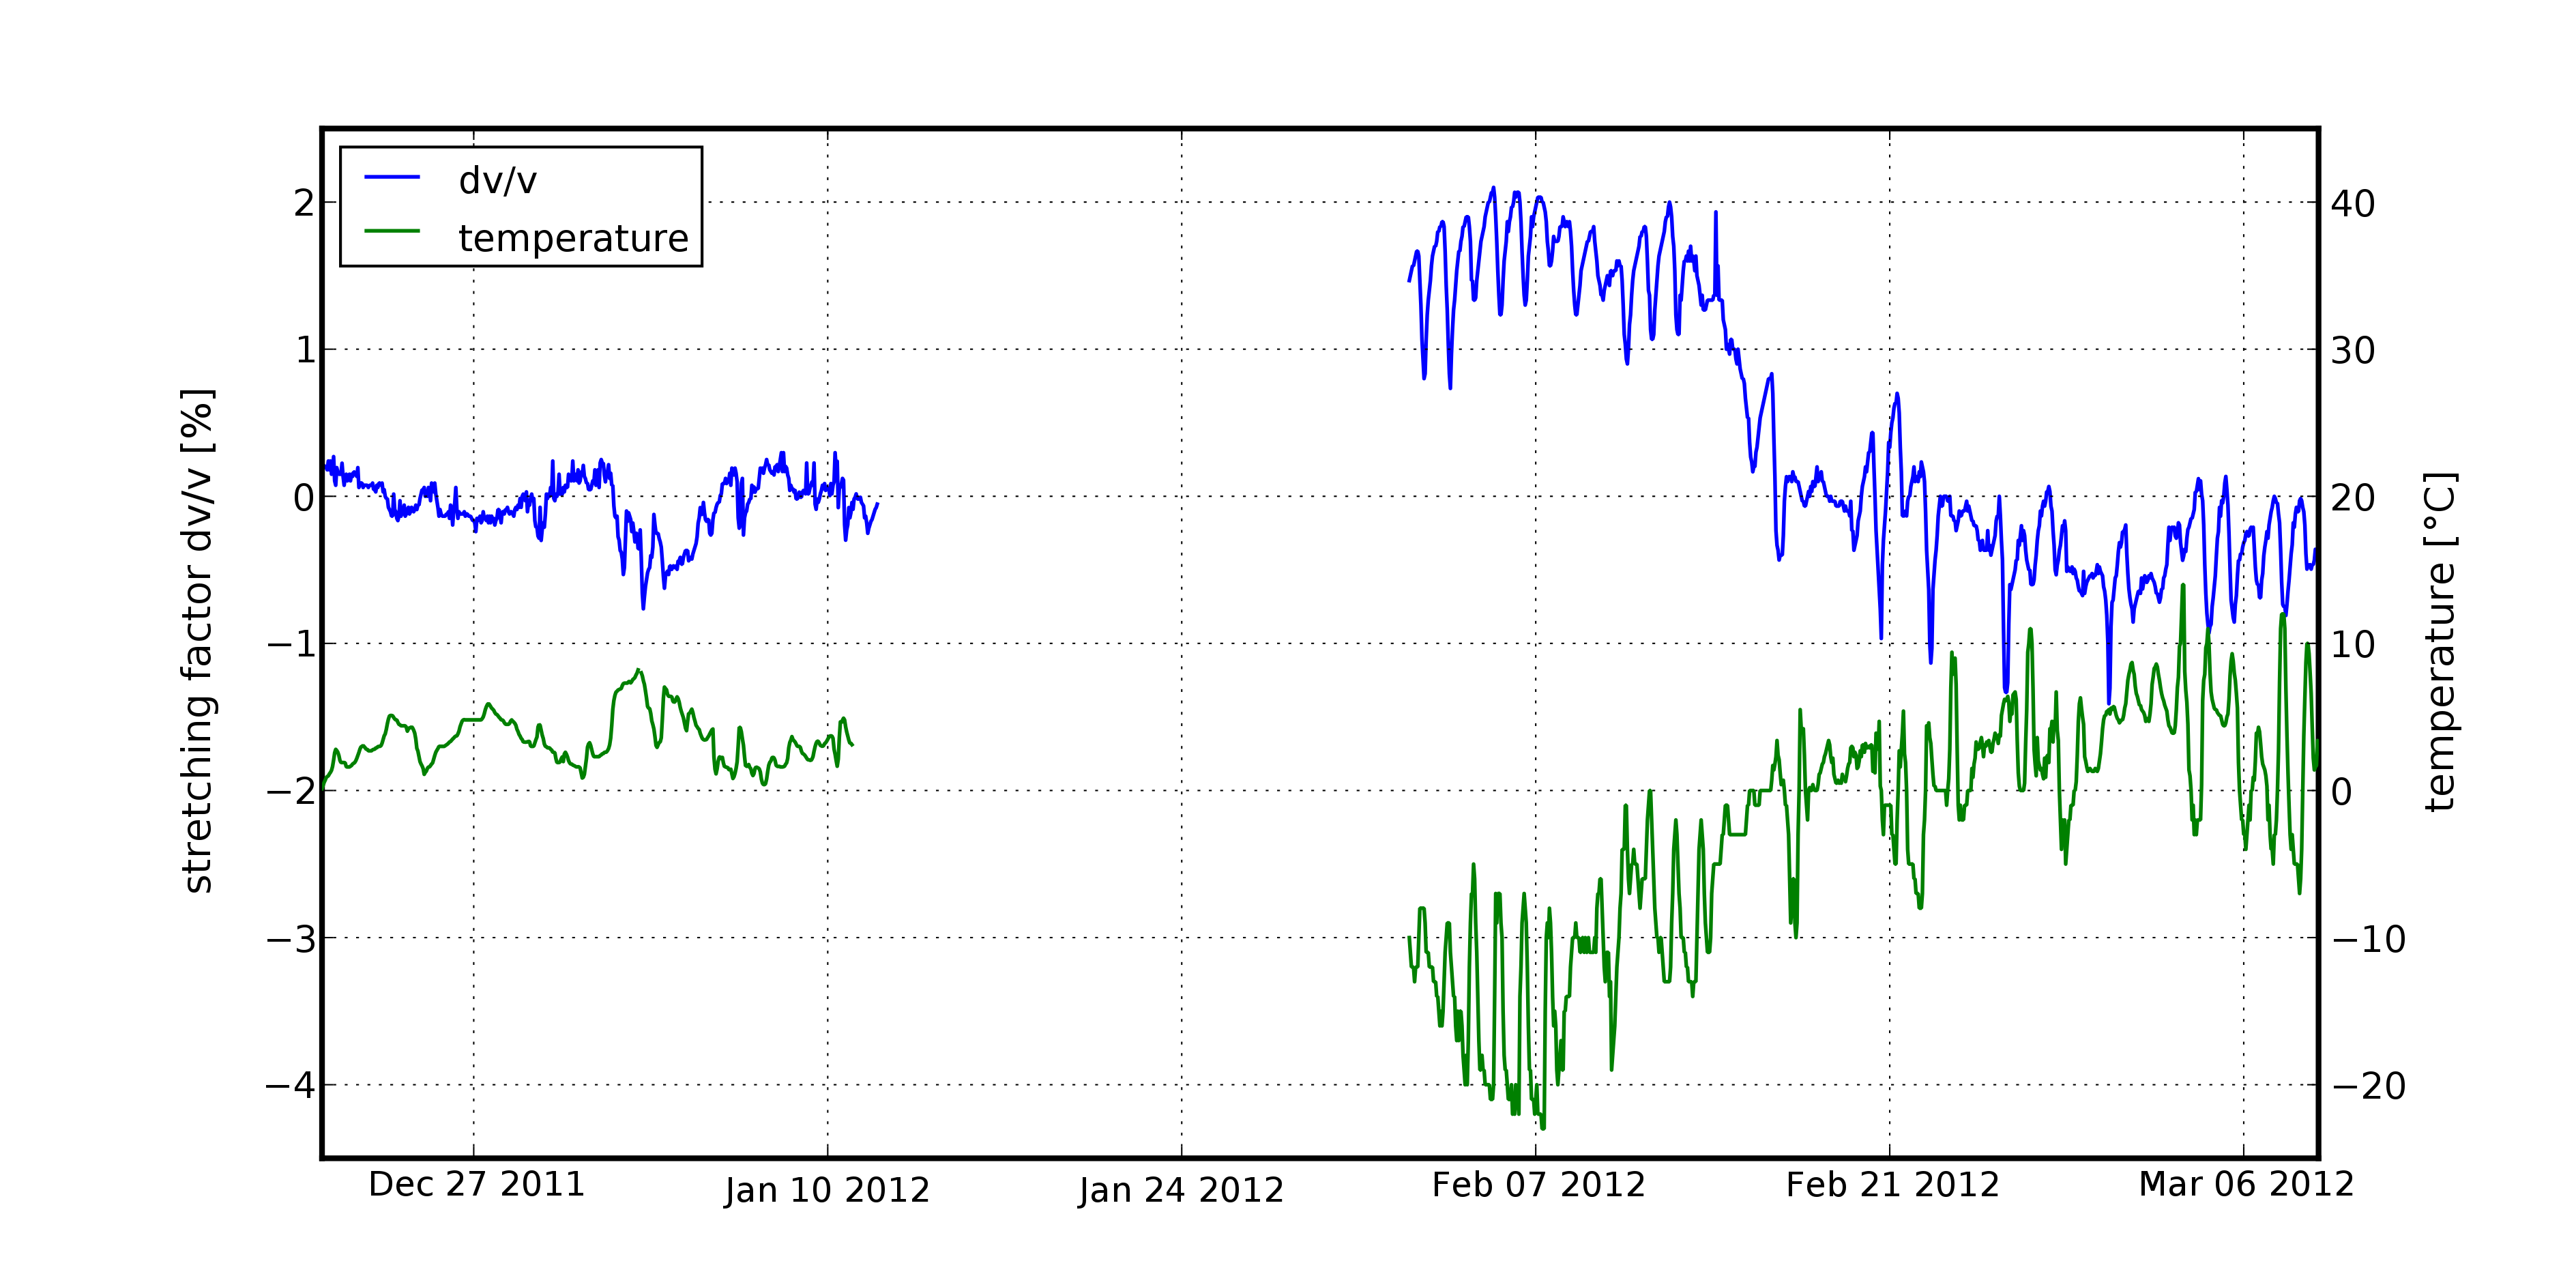
\includegraphics[width=\linewidth,height=0.89\textheight,keepaspectratio]{Figures/whole2_flip.png}};
			 \node[anchor=south west,inner sep=0] at (-4.5,2.5) {\textbf{\color{blue} Velocity variation $\frac{\Delta v}{v}$}};
			 \node[anchor=south west,inner sep=0] at (1.1,2.5) {\textbf{\color{Green} Temperature}};
			 \node[anchor=south west,inner sep=0] (image) at (-0.3,2.5) {
\includegraphics[width=0.06\linewidth,keepaspectratio]{Figures/vs.png}};
        \end{tikzpicture}
    \end{center}
\end{frame}

\begin{frame}{bla}\frametitle{Observed Results}
	\begin{center}
        \begin{tikzpicture}[overlay]
            \node[anchor=south west,inner sep=0] (image) at (-6,-3.4) {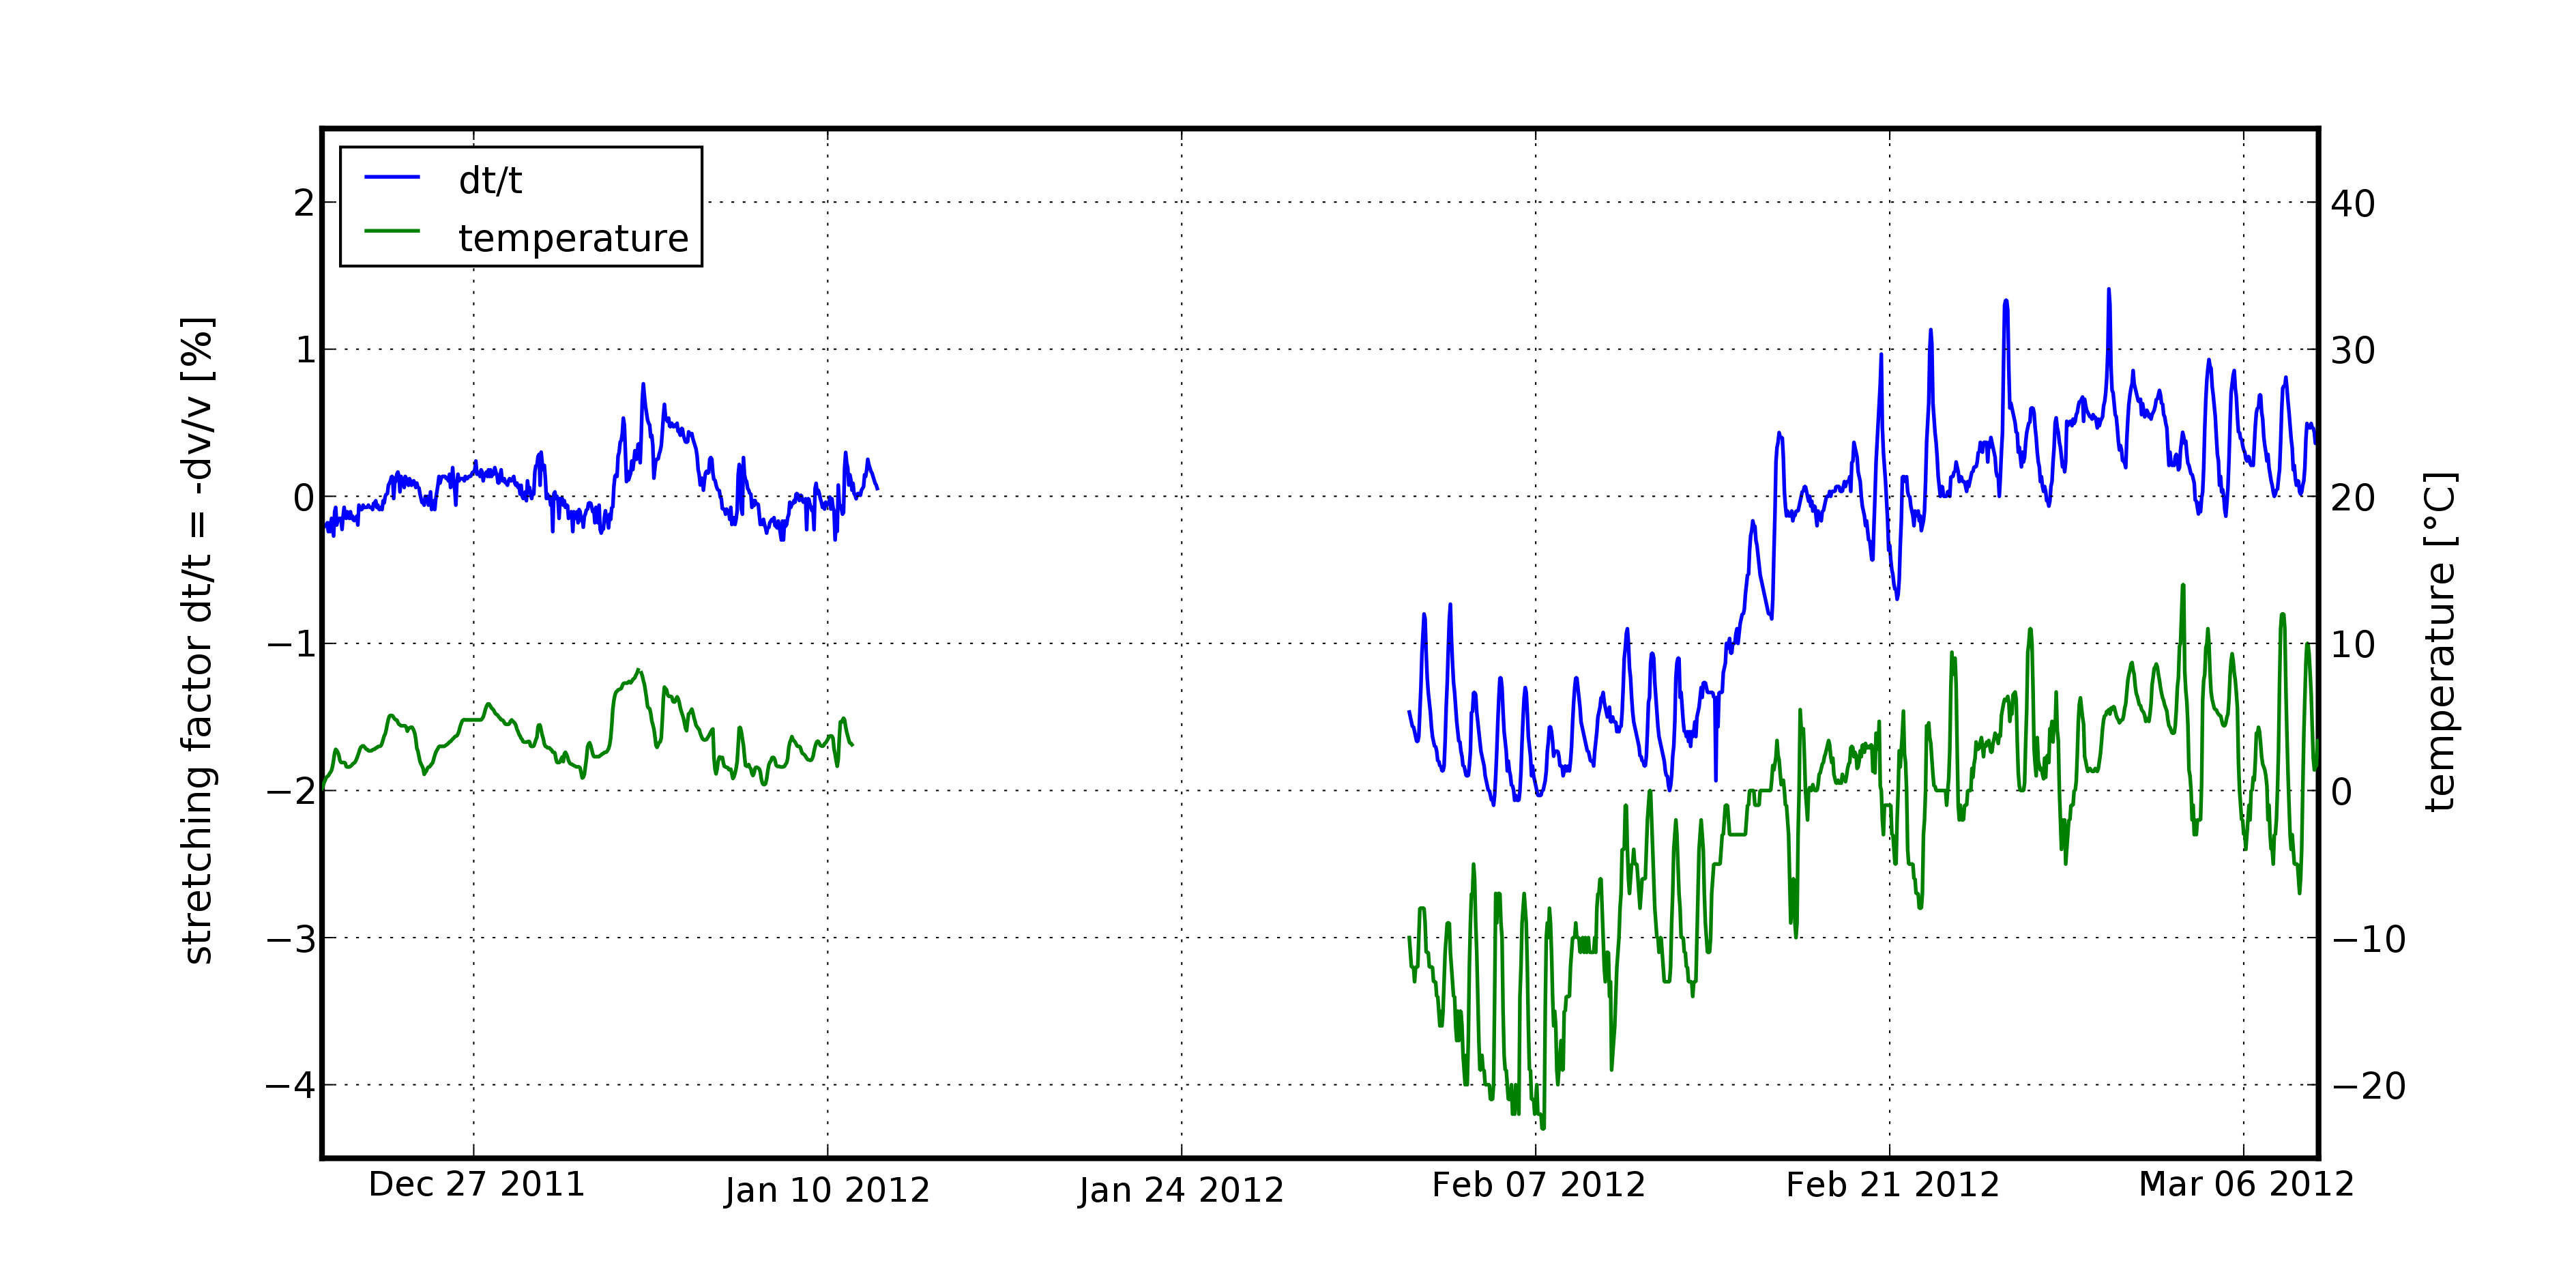
\includegraphics[width=\linewidth,height=0.89\textheight,keepaspectratio]{Figures/whole2.png}};
			 \node[anchor=south west,inner sep=0] at (-4.5,2.5) {\textbf{\color{blue} Velocity variation \color{red} $\frac{\Delta t}{t}$}};
			 \node[anchor=south west,inner sep=0] at (1.1,2.5) {\textbf{\color{Green} Temperature}};
			 \node[anchor=south west,inner sep=0] (image) at (-0.3,2.5) {
\includegraphics[width=0.06\linewidth,keepaspectratio]{Figures/vs.png}};
        \end{tikzpicture}
    \end{center}
\end{frame}

\begin{frame}{bla}\frametitle{Observed Results}
	\begin{center}
        \begin{tikzpicture}[overlay]
            \node[anchor=south west,inner sep=0] (image) at (-6,-3.4) {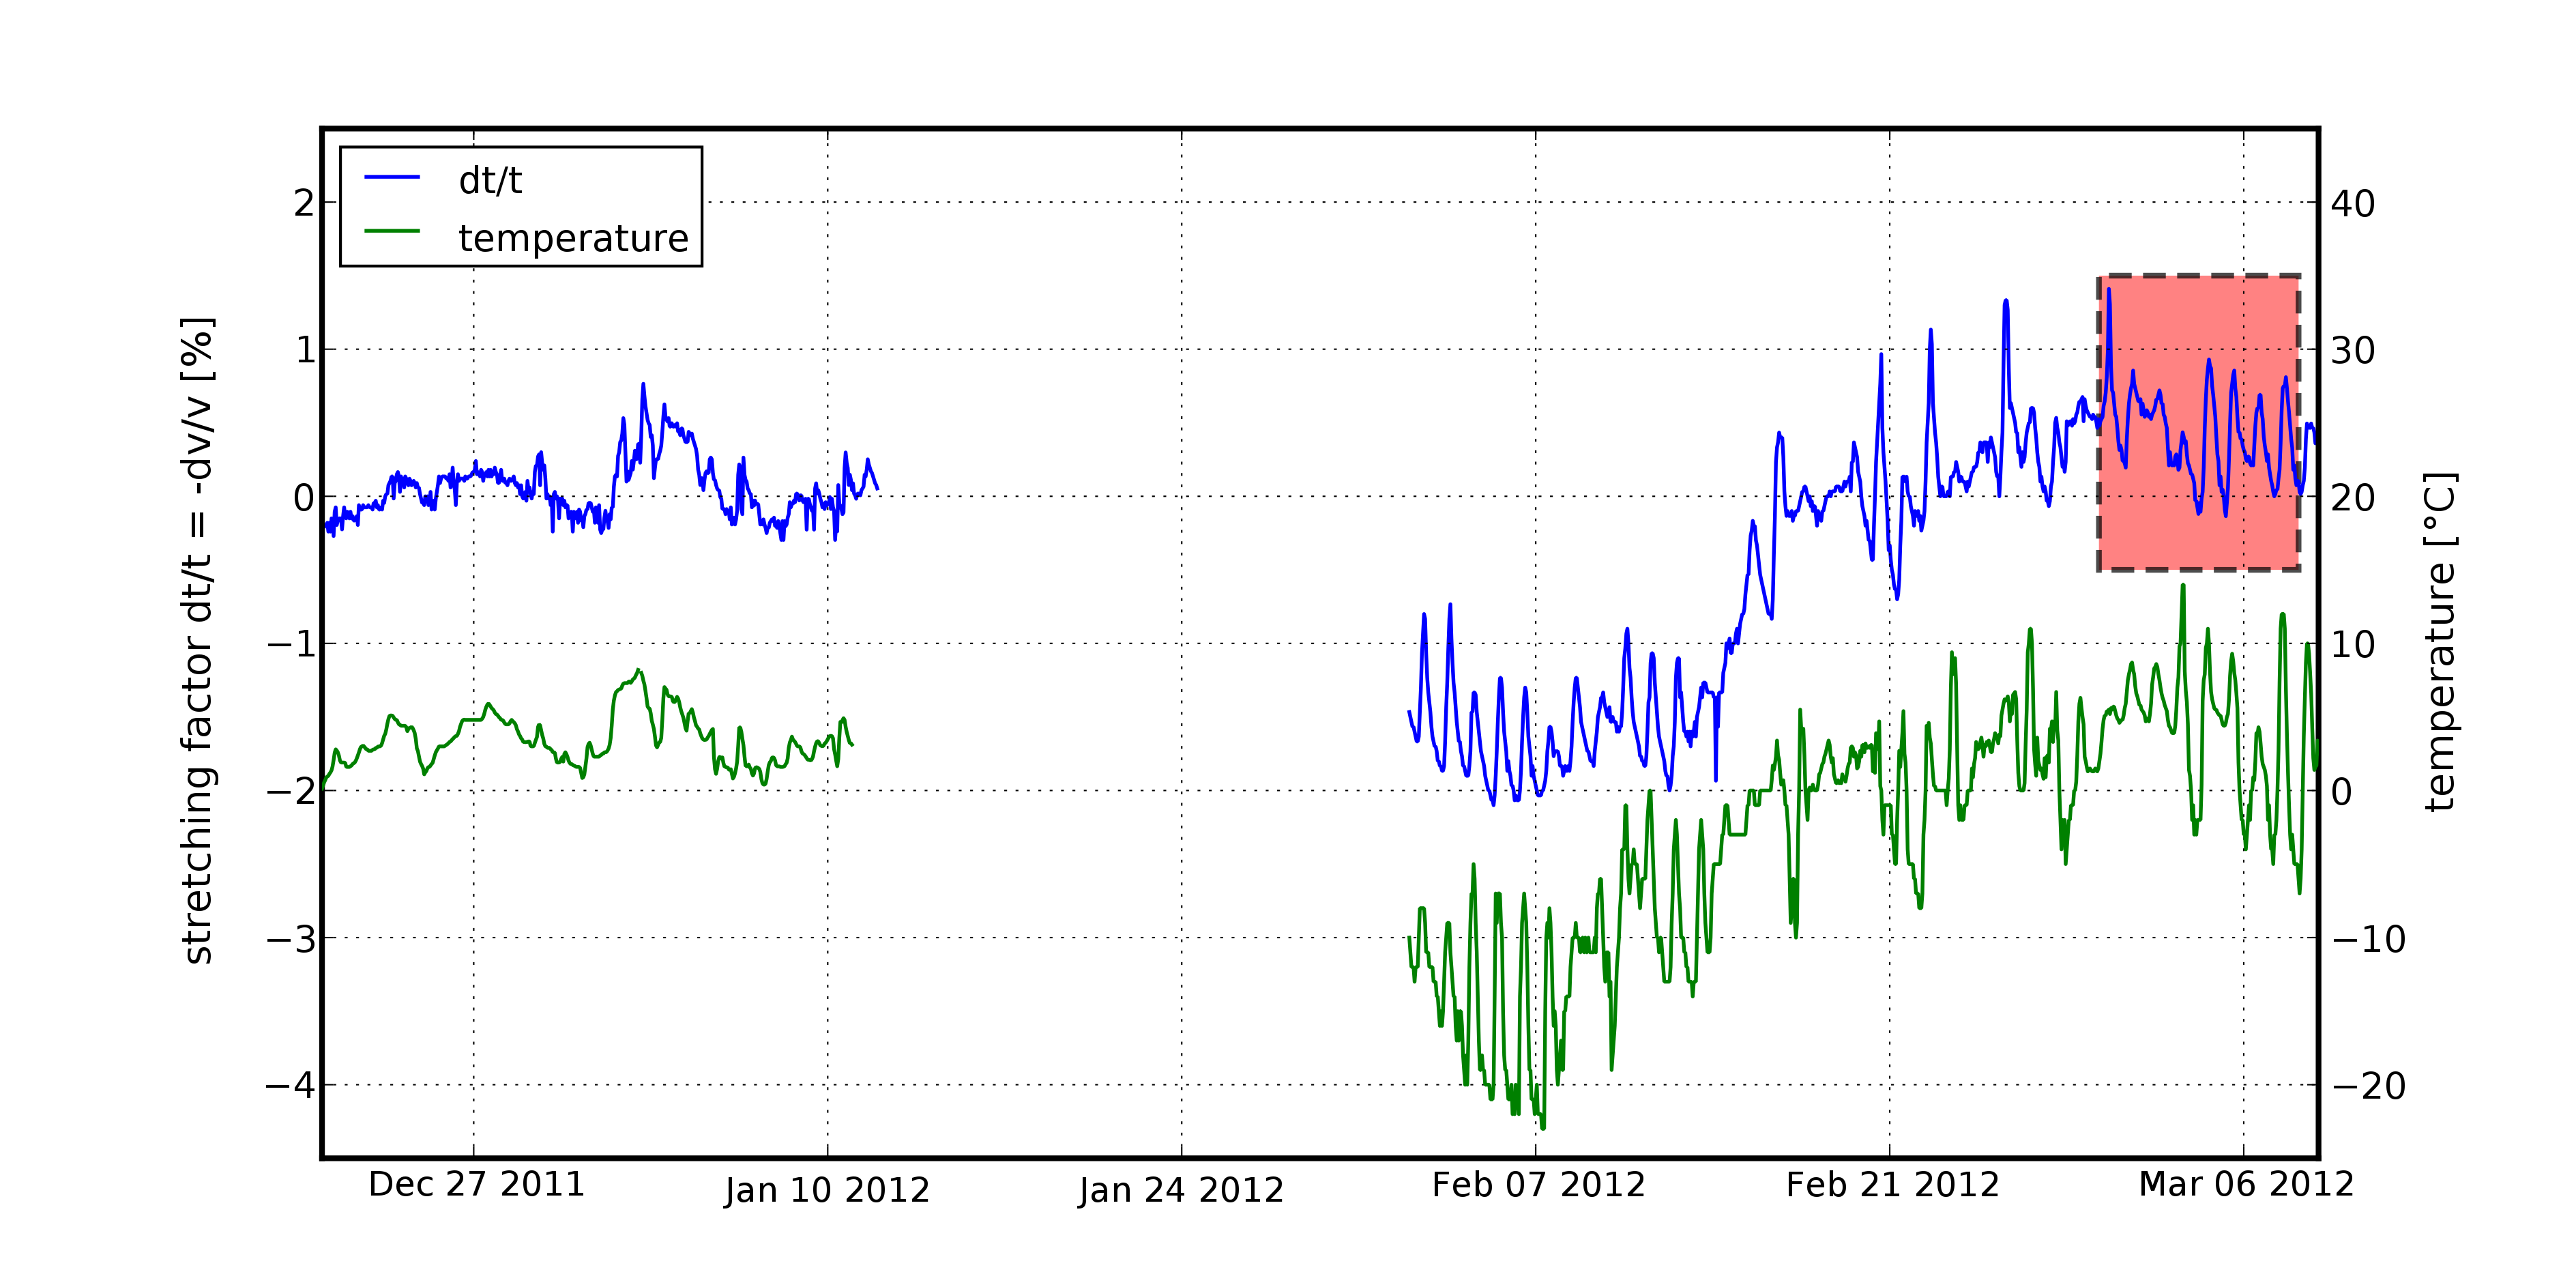
\includegraphics[width=\linewidth,height=0.89\textheight,keepaspectratio]{Figures/whole3_altern.png}};
			 \node[anchor=south west,inner sep=0] at (-4.5,2.5) {\textbf{\color{blue} Velocity variation $\frac{\Delta t}{t}$}};
			 \node[anchor=south west,inner sep=0] at (1.1,2.5) {\textbf{\color{Green} Temperature}};
			 \node[anchor=south west,inner sep=0] (image) at (-0.3,2.5) {
\includegraphics[width=0.06\linewidth,keepaspectratio]{Figures/vs.png}};
        \end{tikzpicture}
    \end{center}
\end{frame}

% =============================================================================

\subsection{Velocity variations II}

\begin{frame}{bla}\frametitle{March 2012}
	\begin{center}
        \begin{tikzpicture}[overlay]
            \node[anchor=south west,inner sep=0] (image) at (-6.1,-3.5) 	{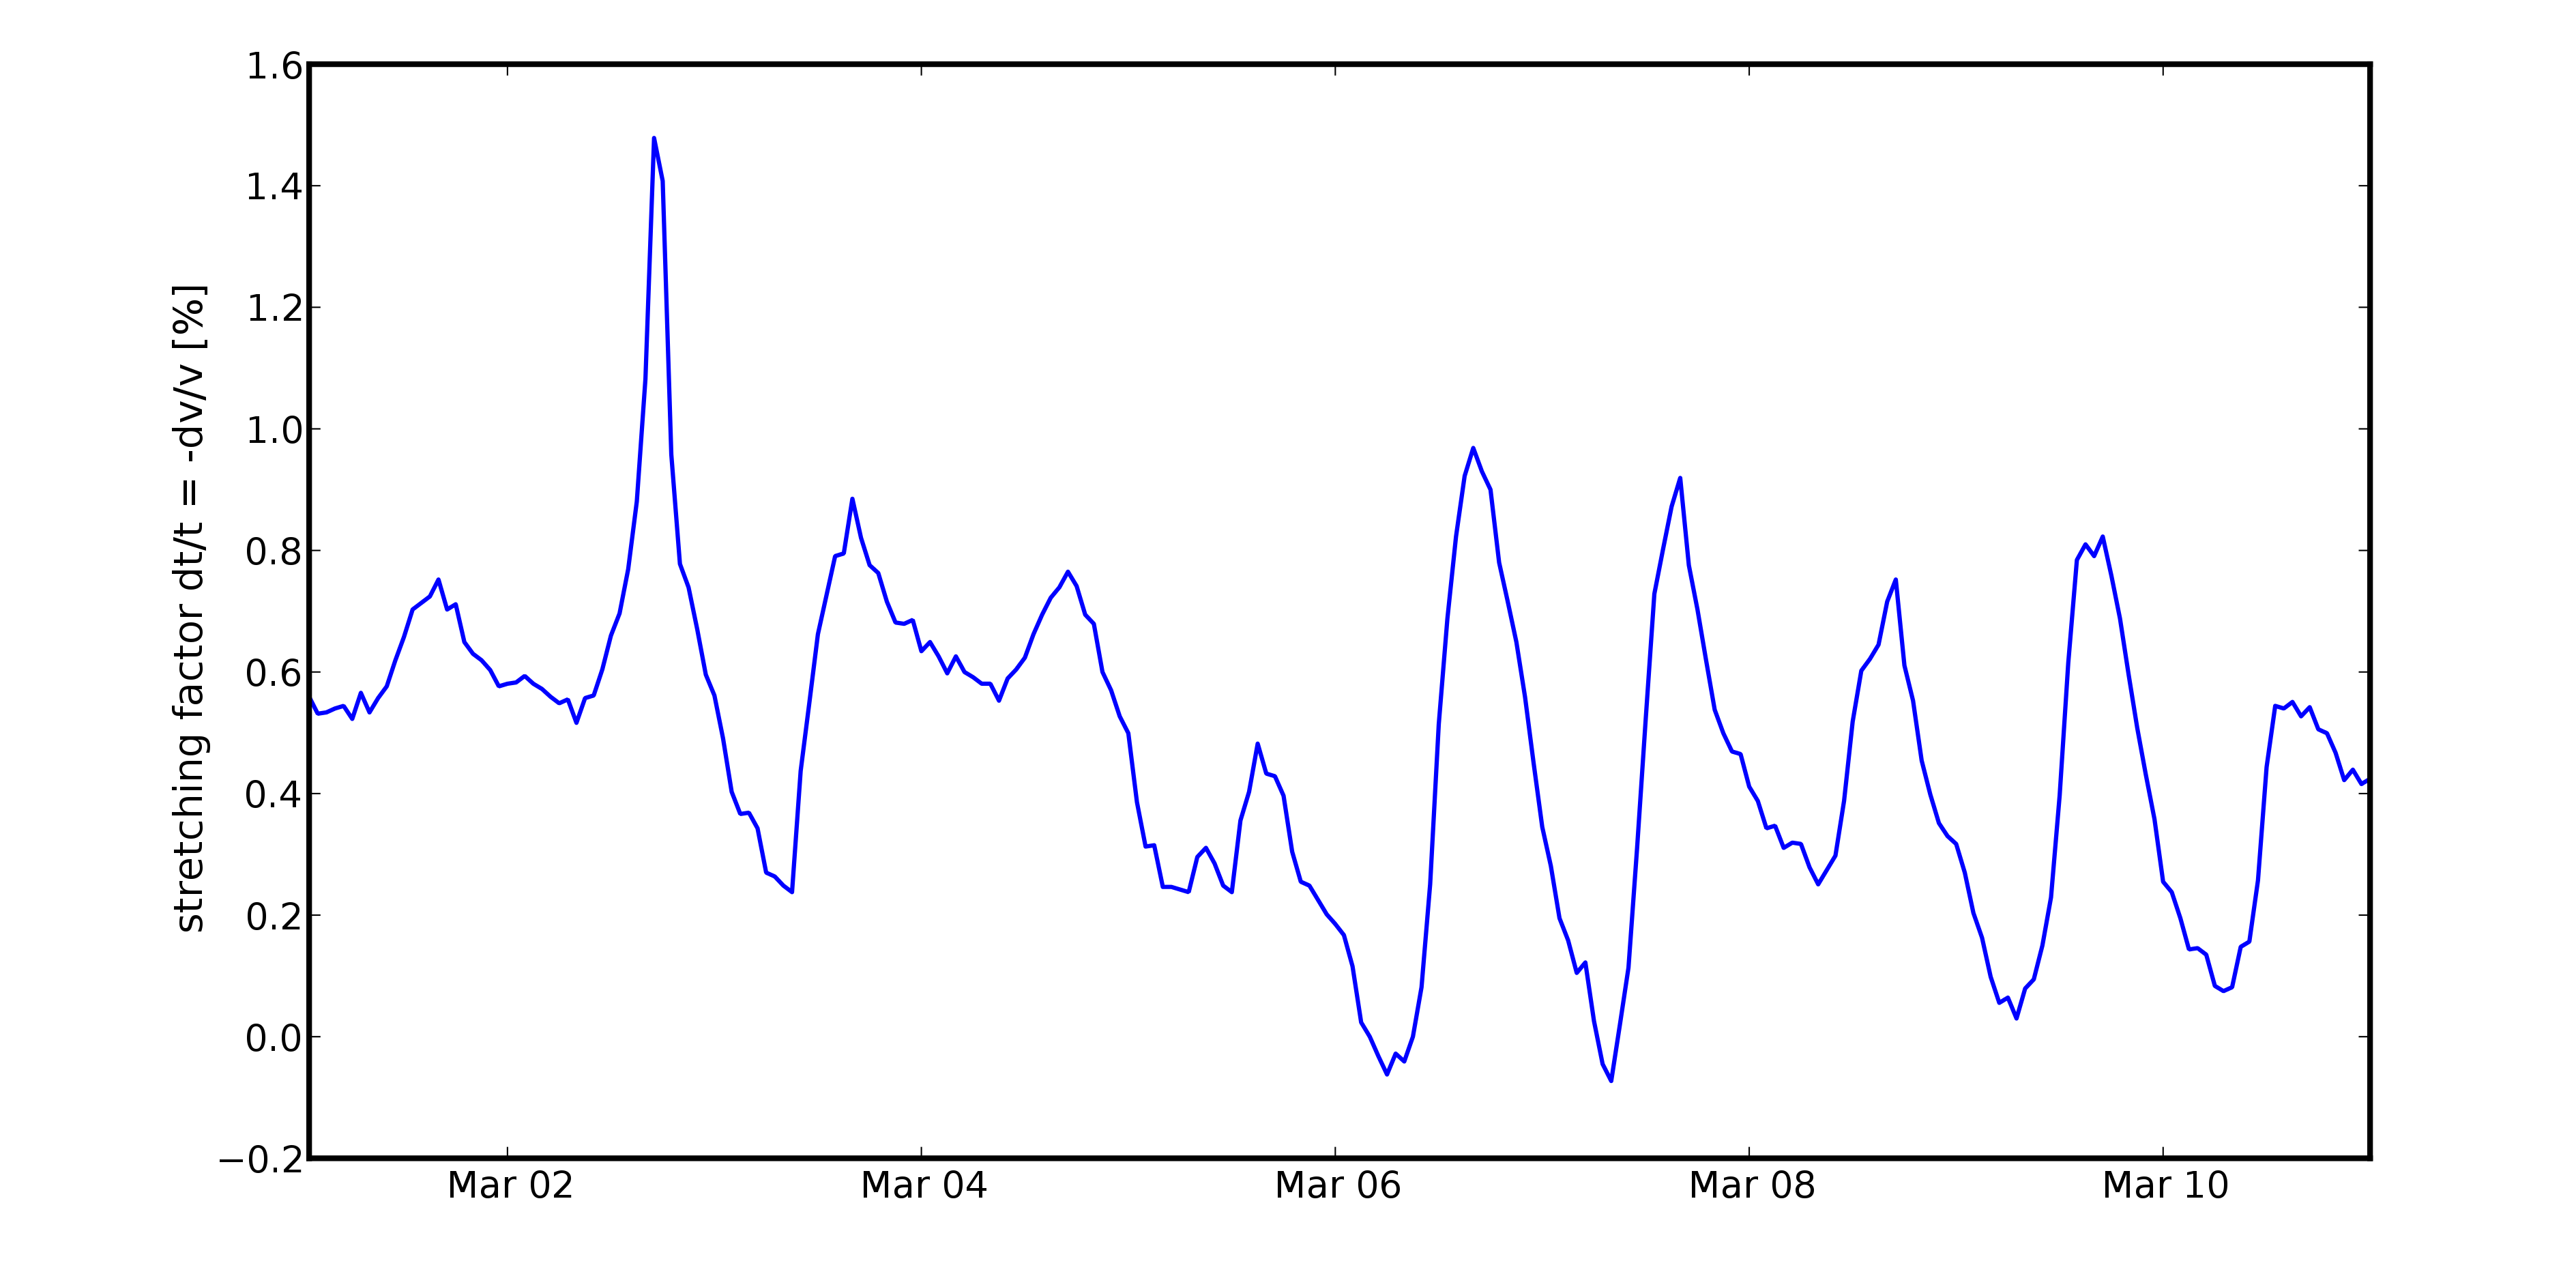
\includegraphics[width=\linewidth,height=0.89\textheight,keepaspectratio]{Figures/stretch_MAR1.png}};
            \node[anchor=south west,inner sep=0] at (-6,2.5) {\textbf{\color{blue} Velocity variation $\frac{\Delta t}{t}$}};
        \end{tikzpicture}
    \end{center}
\end{frame}

\begin{frame}{bla}\frametitle{March 2012}
	\begin{center}
        \begin{tikzpicture}[overlay]
            \node[anchor=south west,inner sep=0] (image) at (-6.1,-3.5) 	{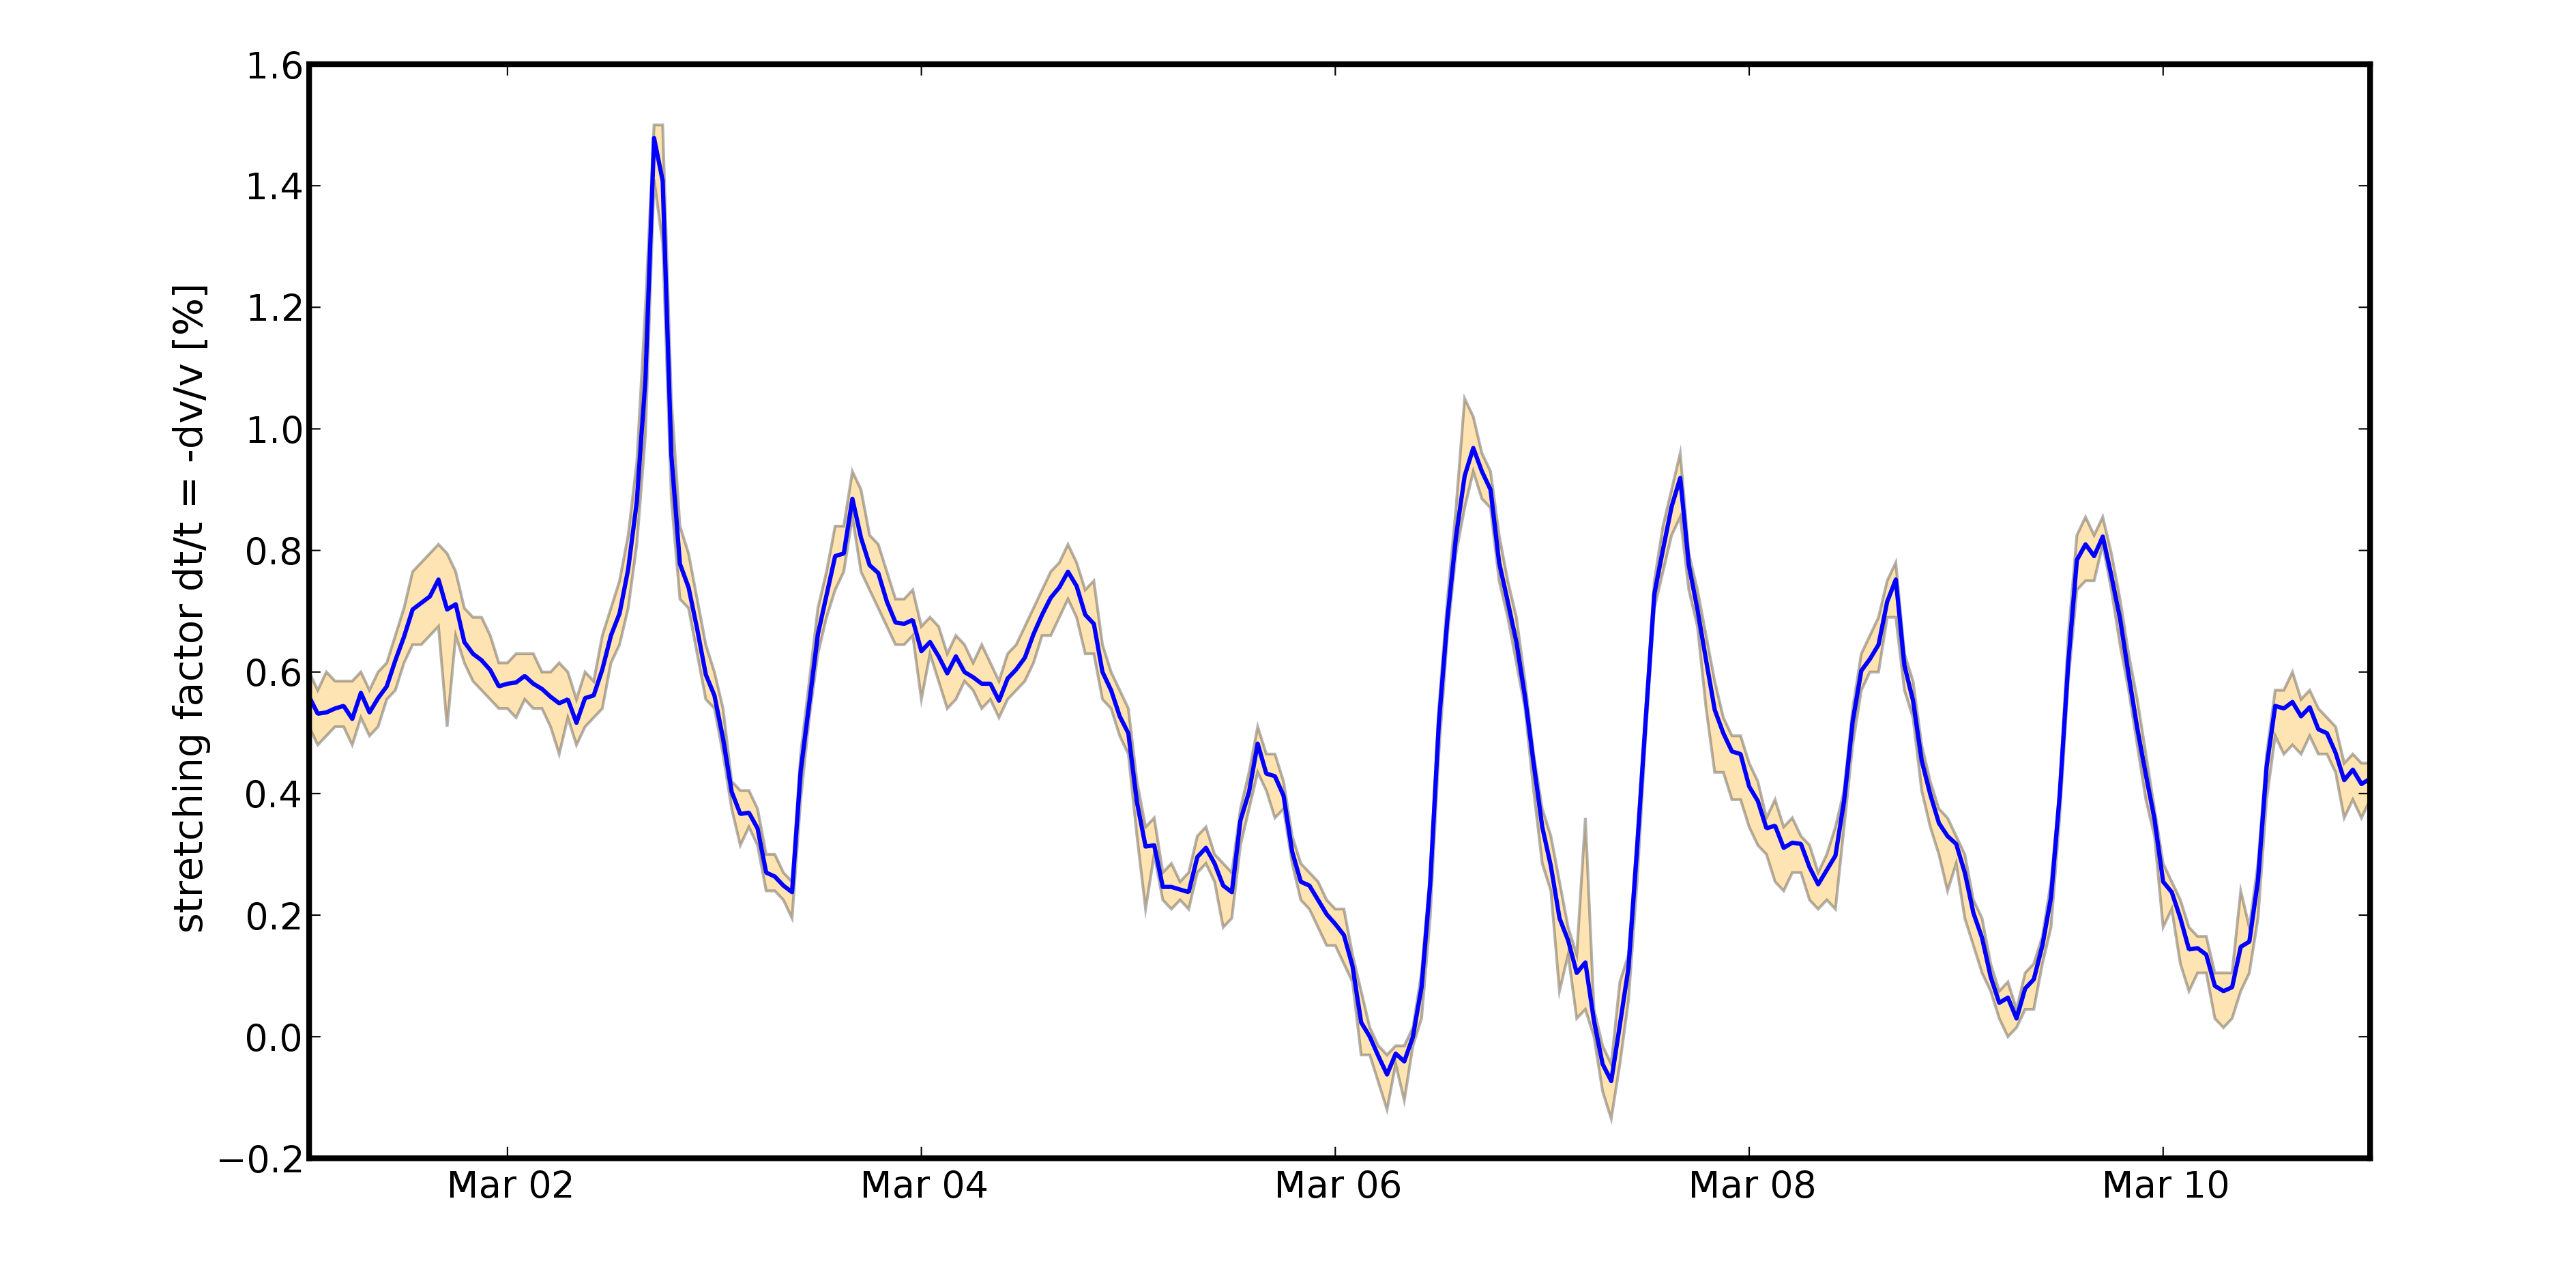
\includegraphics[width=\linewidth,height=0.89\textheight,keepaspectratio]{Figures/stretch_MAR2.png}};
            \node[anchor=south west,inner sep=0] at (-6,2.5) {\textbf{\color{blue} Velocity variation $\frac{\Delta t}{t}$}};
            \node[anchor=south west,inner sep=0] at (-5.2,2) {\textbf{\color{black!40} Deviation}};
            \node[anchor=south west,inner sep=0] at (-6,1.5) {\textbf{\color{black!40} (32 receiver pairs)}};
        \end{tikzpicture}
    \end{center}
\end{frame}

\begin{frame}{bla}\frametitle{March 2012}
	\begin{center}
        \begin{tikzpicture}[overlay]
            \node[anchor=south west,inner sep=0] (image) at (-6.1,-3.5) 	{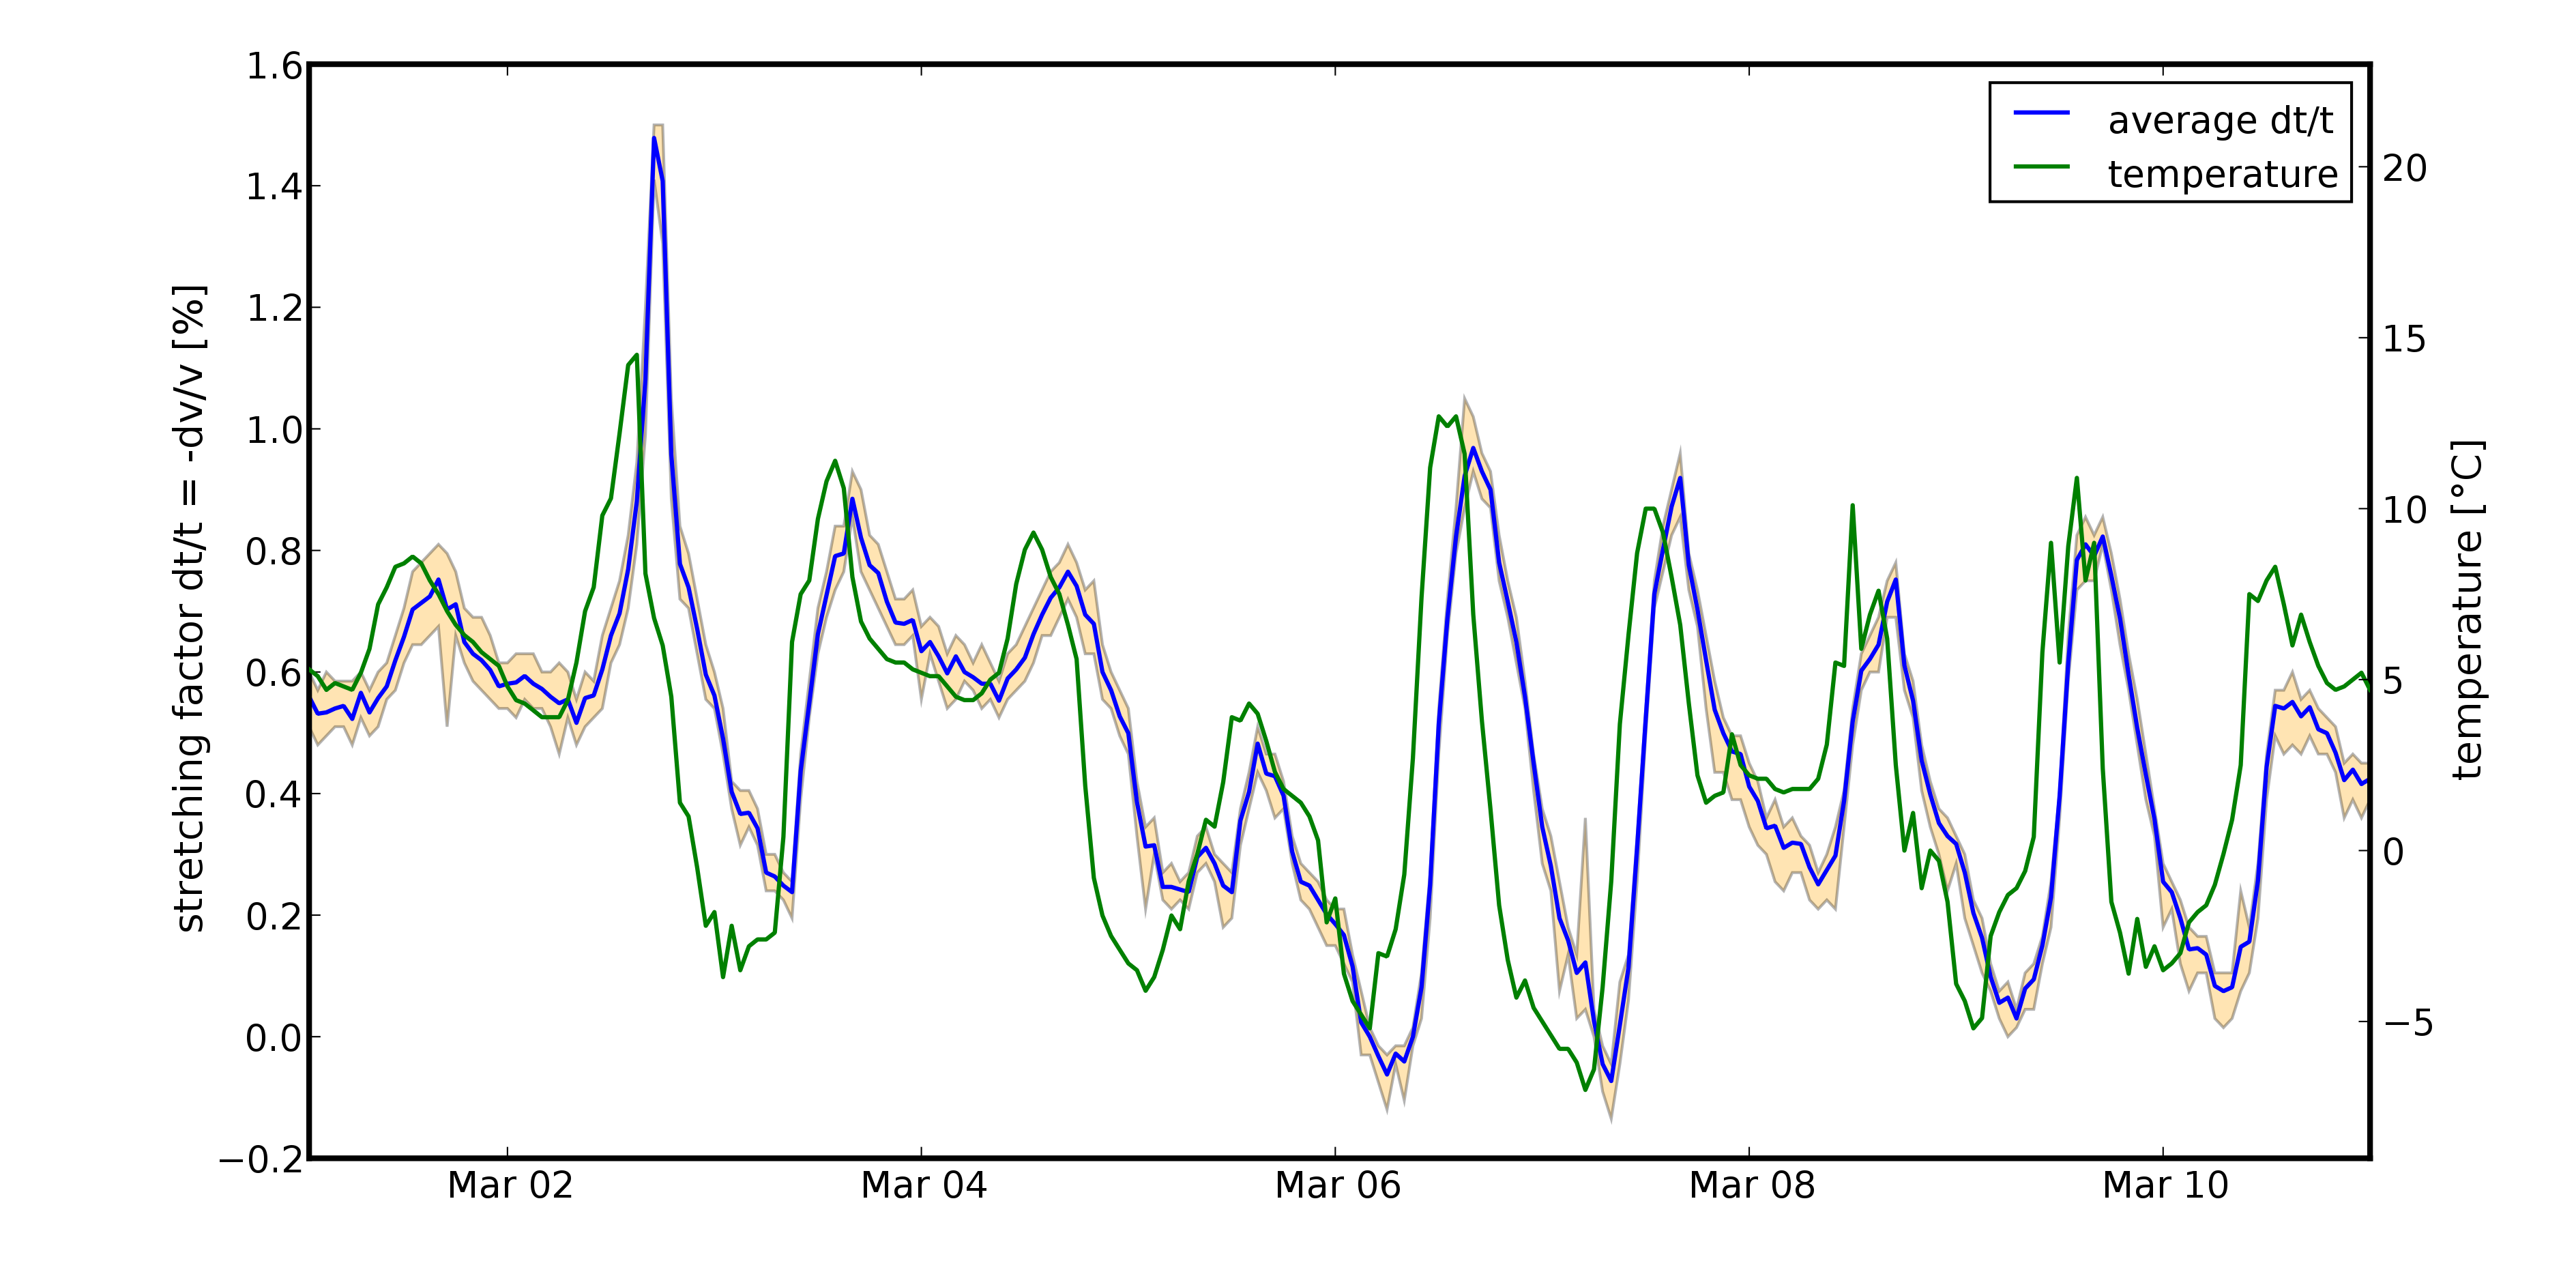
\includegraphics[width=\linewidth,height=0.89\textheight,keepaspectratio]{Figures/stretch_MAR3.png}};
            \node[anchor=south west,inner sep=0] at (-6,2.5) {\textbf{\color{blue} Velocity variation $\frac{\Delta t}{t}$}};
            \node[anchor=south west,inner sep=0] at (-5.2,2) {\textbf{\color{black!40} Deviation}};
            \node[anchor=south west,inner sep=0] at (-6,1.5) {\textbf{\color{black!40} (32 receiver pairs)}};
            \node[anchor=south west,inner sep=0] at (-1,2.5) {\textbf{\color{Green} Temperature}};
        \end{tikzpicture}
    \end{center}
\end{frame}

\begin{frame}{bla}\frametitle{March 2012}
	\begin{center}
        \begin{tikzpicture}[overlay]
            \node[anchor=south west,inner sep=0] (image) at (-6.1,-3.5) 	{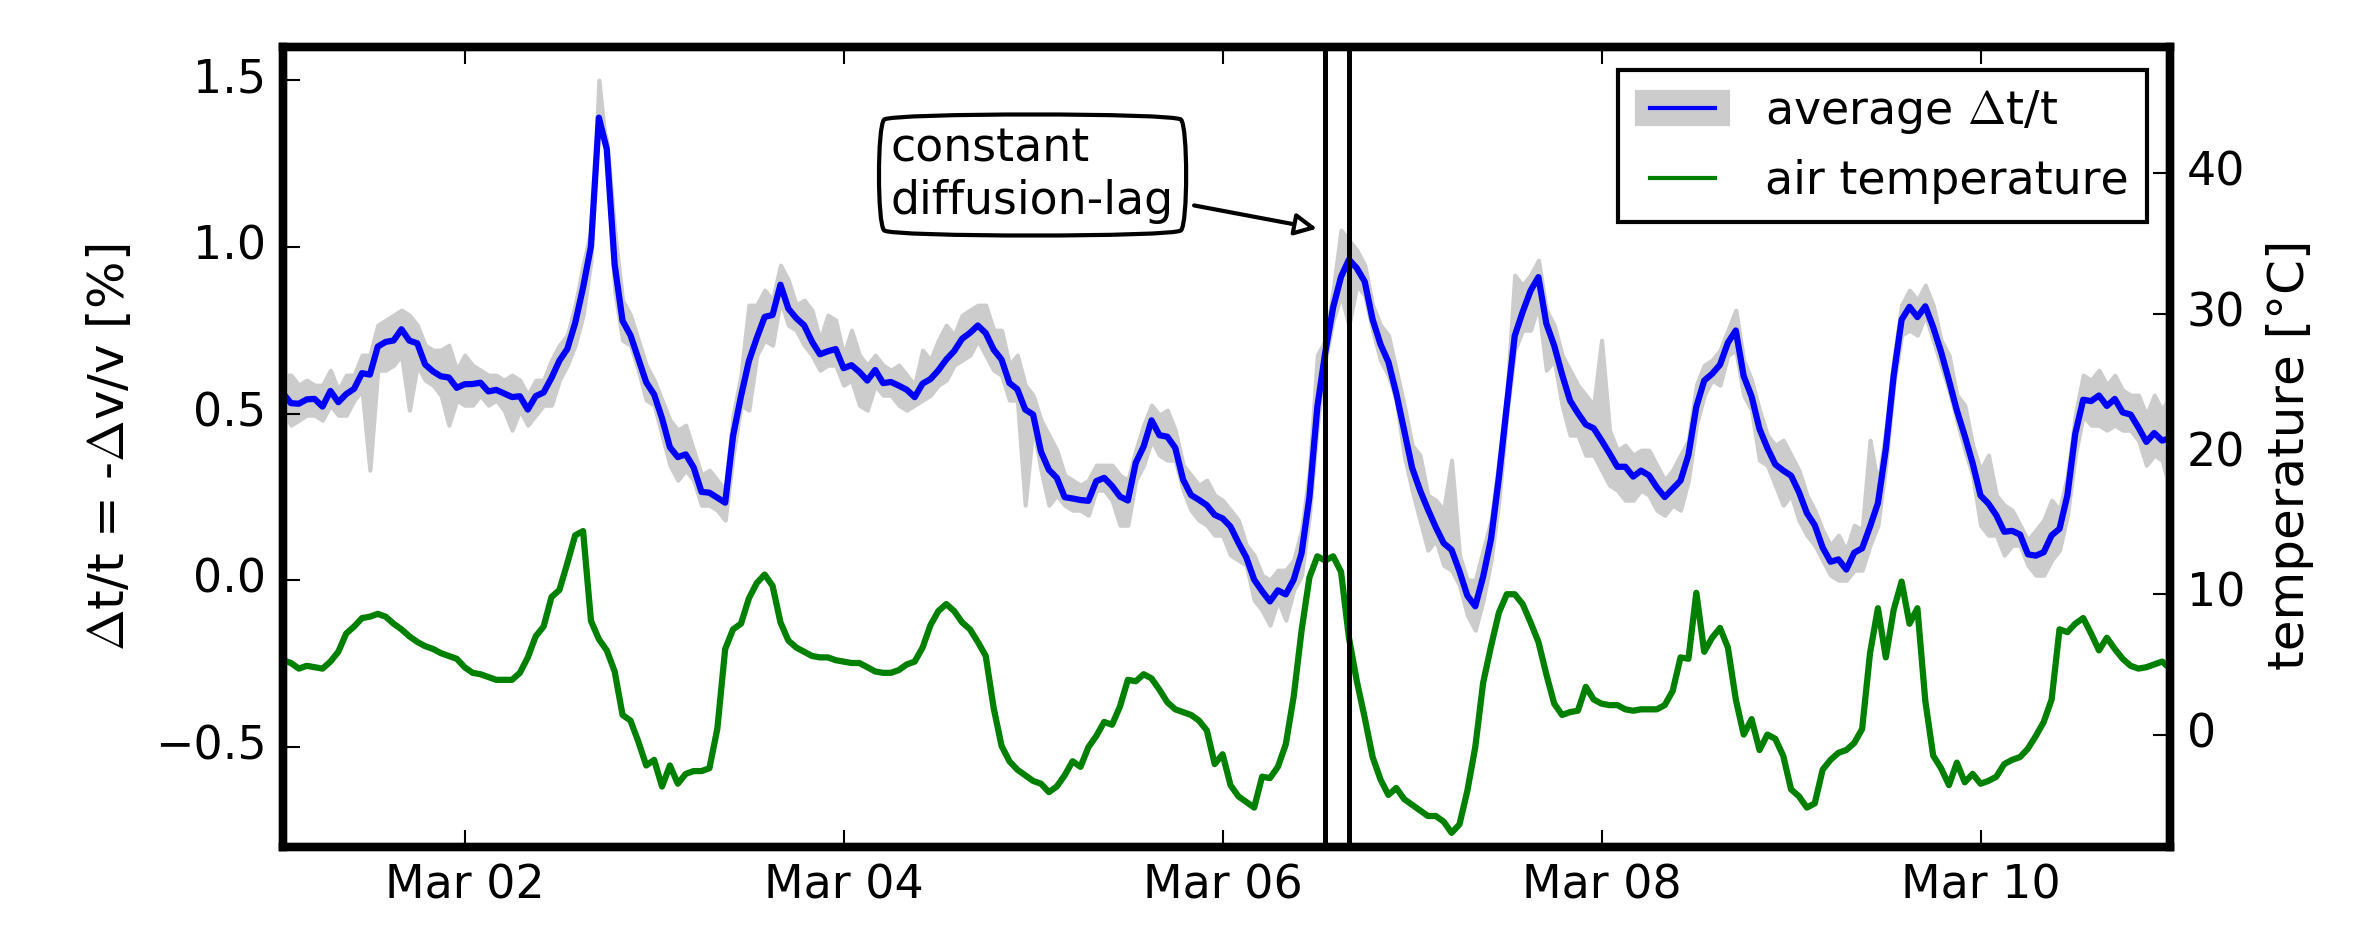
\includegraphics[width=\linewidth,height=0.89\textheight,keepaspectratio]{Figures/stretch_MAR4.png}};
            \node[anchor=south west,inner sep=0] at (-6,2.5) {\textbf{\color{blue} Velocity variation $\frac{\Delta t}{t}$}};
            \node[anchor=south west,inner sep=0] at (-5.2,2) {\textbf{\color{black!40} Deviation}};
            \node[anchor=south west,inner sep=0] at (-6,1.5) {\textbf{\color{black!40} (32 receiver pairs)}};
            \node[anchor=south west,inner sep=0] at (-1,2.5) {\textbf{\color{Green} Temperature}};
        \end{tikzpicture}
    \end{center}
\end{frame}

\begin{frame}{bla}\frametitle{March 2012}
	\begin{center}
        \begin{tikzpicture}[overlay]
            \node[anchor=south west,inner sep=0] (image) at (-6.1,-3.5) 	{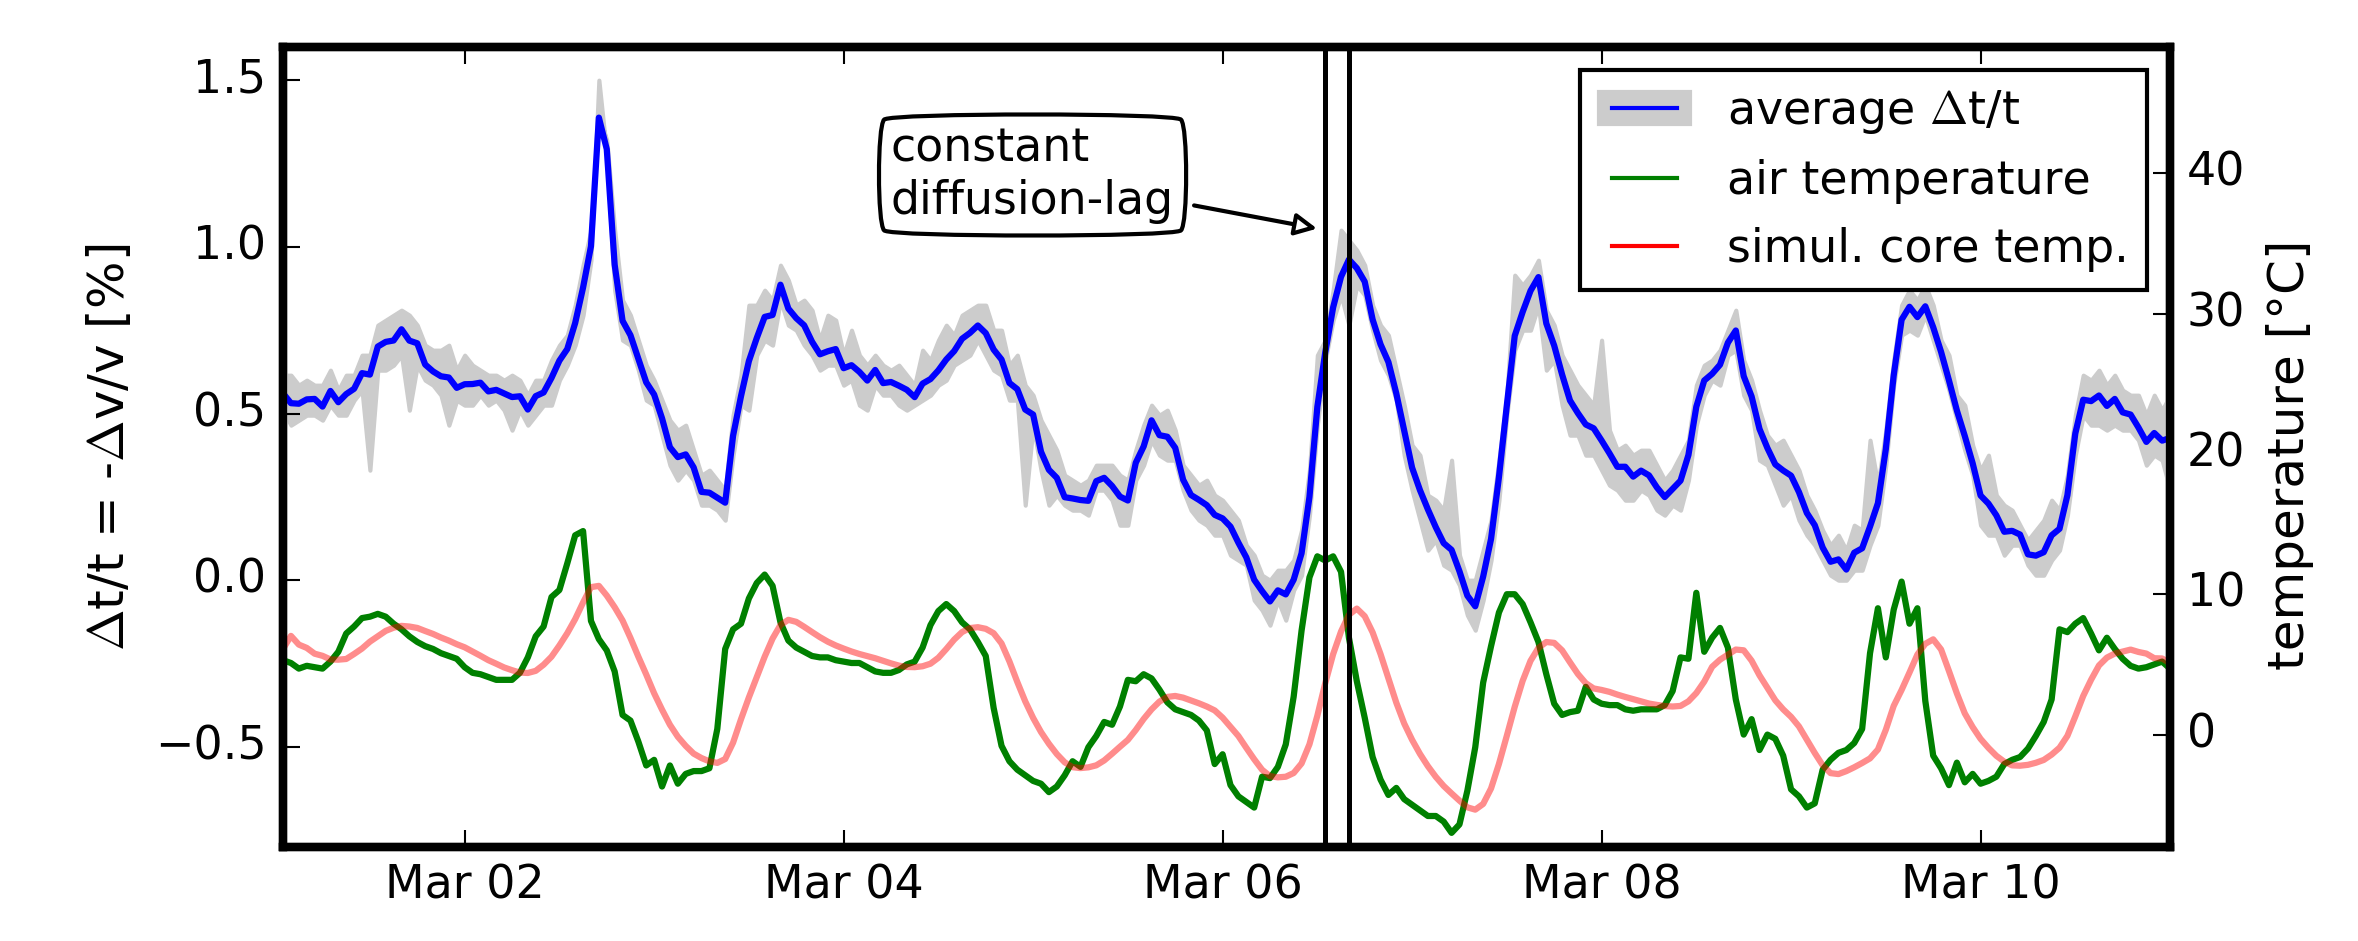
\includegraphics[width=\linewidth,height=0.89\textheight,keepaspectratio]{Figures/stretch_MAR5.png}};
            \node[anchor=south west,inner sep=0] at (-6,2.5) {\textbf{\color{blue} Velocity variation $\frac{\Delta t}{t}$}};
            \node[anchor=south west,inner sep=0] at (-5.2,2) {\textbf{\color{black!40} Deviation}};
            \node[anchor=south west,inner sep=0] at (-6,1.5) {\textbf{\color{black!40} (32 receiver pairs)}};
            \node[anchor=south west,inner sep=0] at (-1,2.5) {\textbf{\color{Green} Temperature}};
            \node[anchor=south west,inner sep=0] at (3,2.5) {\textbf{\color{red!40} Simulated core}};
            \node[anchor=south west,inner sep=0] at (3.2,2) {\textbf{\color{red!40} temperature}};
        \end{tikzpicture}
    \end{center}
\end{frame}

\begin{frame}{bla}\frametitle{March 2012}
	\begin{center}
        \begin{tikzpicture}[overlay]
            \node[anchor=south west,inner sep=0] (image) at (-6.1,-3.5) 	{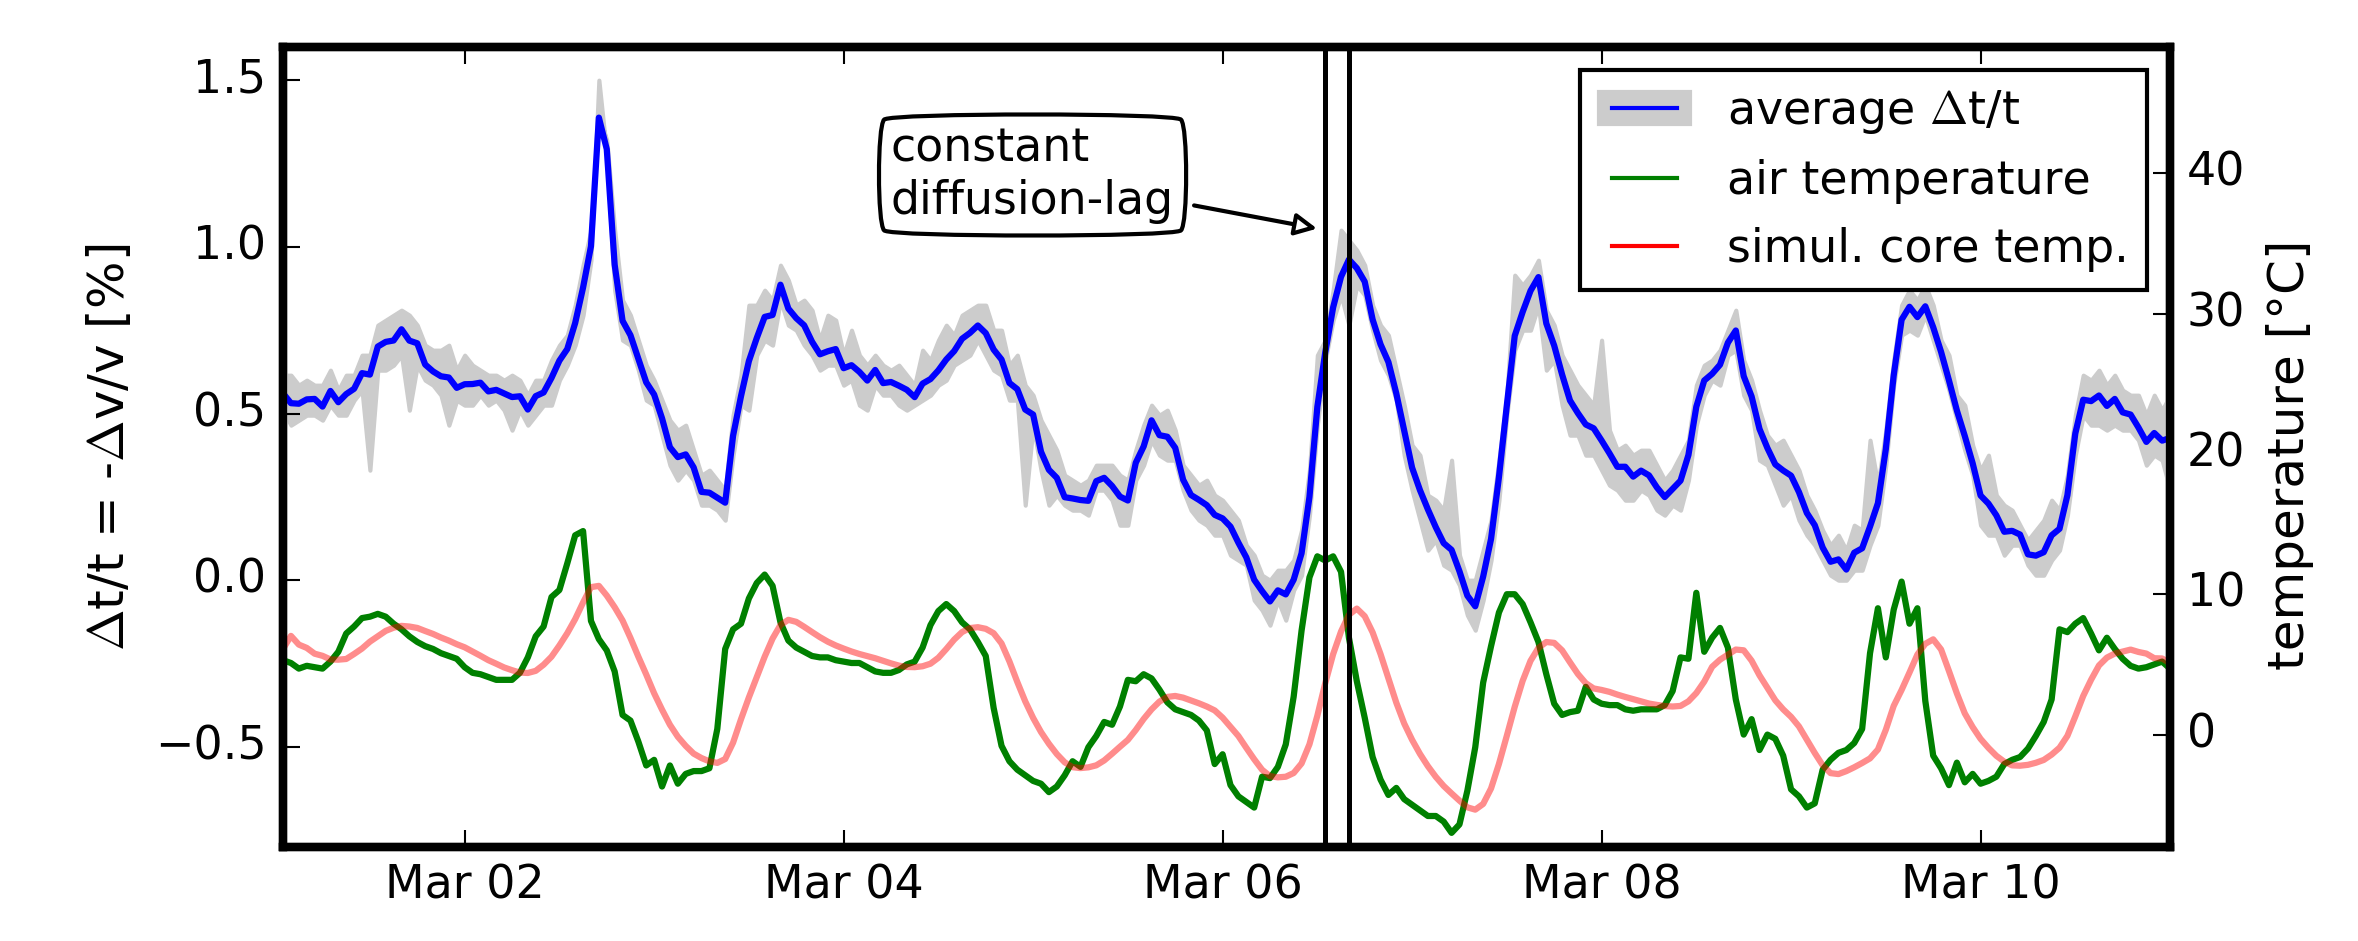
\includegraphics[width=\linewidth,height=0.89\textheight,keepaspectratio]{Figures/stretch_MAR5.png}};
            \node[anchor=south west,inner sep=0] at (-6,2.5) {\textbf{\color{blue} Velocity variation $\frac{\Delta t}{t}$}};
            \node[anchor=south west,inner sep=0] at (-5.2,2) {\textbf{\color{black!40} Deviation}};
            \node[anchor=south west,inner sep=0] at (-6,1.5) {\textbf{\color{black!40} (32 receiver pairs)}};
            \node[anchor=south west,inner sep=0] at (-1,2.5) {\textbf{\color{Green} Temperature}};
            \node[anchor=south west,inner sep=0] at (3,2.5) {\textbf{\color{red!40} Simulated core}};
            \node[anchor=south west,inner sep=0] at (3.2,2) {\textbf{\color{red!40} temperature}};
            \node[anchor=south west,inner sep=0] at (-3.5,-2.3) {\begin{tcolorbox}[colback=green!5,colframe=salve@blue,title=Overall Results,width=7cm]
            		    \begin{small}
							\begin{tabular}{ll}
								$\frac{\Delta v}{v}$  & -1.5$\%$ to +2.1$\%$\\
								&\\
								temperatures & +14${\textdegree}$C to -23${\textdegree}$C\\
								&\\
								average rate & 0.064 $\frac{\%}{{\textdegree}C}$\\
								&\\
								diffusion lag & $\approx$ 3 hours
							
							\end{tabular}
            			\end{small}
					\end{tcolorbox}};
		\end{tikzpicture}
    \end{center}
\end{frame}


\section{Tests}
\subsection{thermalex}
\begin{frame}
	\frametitle{Reliability Tests}
	\begin{center}
		\begin{tikzpicture}[overlay]
            \node[anchor=south west,inner sep=0] (box1) at (-6.2,0) {
            		\begin{tcolorbox}[colback=green!5,colframe=salve@blue,title=Thermal expansion,width=8cm]
            		    \begin{small}
            		    Expansion/Contraction of the bridge\\
 {\color{green!5}
 $\Rightarrow$ Effect in the order of \textbf{6-14 $\mathbf{\cdot 10^{-4}}$ $\frac{\%}{\textdegree{C}}$} for steel-reinforced concrete}
            			\end{small}
					\end{tcolorbox}};
			\node[anchor=south west,inner sep=0] (box2) at (-6.2,-3.5) {
            		\begin{tcolorbox}[colback=green!5,colframe=salve@blue,title=Instrument stability,width=8cm]
            		    \begin{small}
 Temperature dependence of geophones\\
 {\color{green!5} $\Rightarrow$ Apparent delay of max.											\textbf{0.52 \%} for extreme shifts in corner frequency.}
            			\end{small}
					\end{tcolorbox}};
			\node[anchor=south west,inner sep=0] (box3) at (2.7,-1.2) {
            		\begin{tcolorbox}[colback=green!5,colframe=salve@blue,title=Msmt range ,width=3.5cm]
            		    \begin{small}
\textbf{-1.5 to +2.3 \%}
            			\end{small}
					\end{tcolorbox}};
        \end{tikzpicture}
   \end{center}
\end{frame}

\begin{frame}
	\frametitle{Reliability Tests}
	\begin{center}
		\begin{tikzpicture}[overlay]
            \node[anchor=south west,inner sep=0] (box1) at (-6.2,0) {
            		\begin{tcolorbox}[colback=green!5,colframe=green,title=Thermal expansion,width=8cm]
            		    \begin{small}
            		    Expansion/Contraction of the bridge\\
 $\Rightarrow$ Effect in the order of \textbf{6-14 $\mathbf{\cdot 10^{-4}}$ $\frac{\%}{\textdegree{C}}$} for steel-reinforced concrete
            			\end{small}
					\end{tcolorbox}};
			\node[anchor=south west,inner sep=0] (box2) at (-6.2,-3.5) {
            		\begin{tcolorbox}[colback=green!5,colframe=salve@blue,title=Instrument stability,width=8cm]
            		    \begin{small}
 Temperature dependence of geophones\\
 {\color{green!5}
 $\Rightarrow$ Apparent delay of max.											\textbf{0.52 \%} for extreme shifts in corner frequency.}
            			\end{small}
					\end{tcolorbox}};
			\node[anchor=south west,inner sep=0] (box3) at (2.7,-1.2) {
            		\begin{tcolorbox}[colback=green!5,colframe=salve@blue,title=Msmt range ,width=3.5cm]
            		    \begin{small}
\textbf{-1.5 to +2.3 \%}
            			\end{small}
					\end{tcolorbox}};
			\draw [<->,>=stealth,green,ultra thick,sloped] (box1)-- node[above] {\color{black}\textbf{$\pmb{\ll}$}} ++(box3);

        \end{tikzpicture}
   \end{center}
\end{frame}
%
\begin{frame}
	\frametitle{Reliability Tests}
	\begin{center}
		\begin{tikzpicture}[overlay]
            \node[anchor=south west,inner sep=0] (box1) at (-6.2,0) {
            		\begin{tcolorbox}[colback=green!5,colframe=green,title=Thermal expansion,width=8cm]
            		    \begin{small}
            		    Expansion/Contraction of the bridge\\
 $\Rightarrow$ Effect in the order of \textbf{6-14 $\mathbf{\cdot 10^{-4}}$ $\frac{\%}{\textdegree{C}}$} for steel-reinforced concrete
            			\end{small}
					\end{tcolorbox}};
			\node[anchor=south west,inner sep=0] (box2) at (-6.2,-3.5) {
            		\begin{tcolorbox}[colback=green!5,colframe=green,title=Instrument stability,width=8cm]
            		    \begin{small}
 Temperature dependence of geophones\\
 $\Rightarrow$ Apparent delay of max.											\textbf{0.52 \%} for extreme shifts in corner frequency.
            			\end{small}
					\end{tcolorbox}};
			\node[anchor=south west,inner sep=0] (box3) at (2.7,-1.2) {
            		\begin{tcolorbox}[colback=green!5,colframe=salve@blue,title=Msmt range ,width=3.5cm]
            		    \begin{small}
            		    \textbf{-1.5 to +2.3 \%}
            			\end{small}
					\end{tcolorbox}};
			\draw [<->,>=stealth,green,ultra thick,sloped] (box1)-- node[above] {\color{black}\textbf{$\pmb{\ll}$}} ++(box3);
			\draw [<->,>=stealth,green,ultra thick,sloped] (box2)-- node[below] {\color{black}\textbf{$\pmb{<}$}} ++(box3) ;
        \end{tikzpicture}
   \end{center}
\end{frame}
	
\section{Conclusions}
\subsection{Conclusions}
\begin{frame}
	\frametitle{Conclusions}
	\begin{center}
		\begin{tikzpicture}       
            \node[anchor=south west,inner sep=0] (box2) at (0,0) {
            		\begin{tcolorbox}[colback=green!5,colframe=salve@blue,title=,width=10cm]
            		    \begin{small}
							\begin{itemize}
								\item Resolution of velocity variations is possible via cross-correlations from ambient traffic noise on a bridge
								\item Captured small velocity variations caused by temperature fluctuations:\\
									 relative velocity $\frac{\Delta v}{v}$: -1.5$\%$ to +2.1$\%$\\
									 temperature range: +14${\textdegree}$C to -23${\textdegree}$C
								\item Strong correlation between temperature and $\frac{\Delta v}{v}$ series
								\item Advantages: high temporal resolution, high accuracy, low logistical effort
							\end{itemize}
            			\end{small}
					\end{tcolorbox}};
         \end{tikzpicture}
    \end{center}
\end{frame}

\subsection{Outlook}

\begin{frame}
	\begin{tikzpicture}[overlay]
		\node[anchor=south west,inner sep=0] (image) at (0,1.5) 	{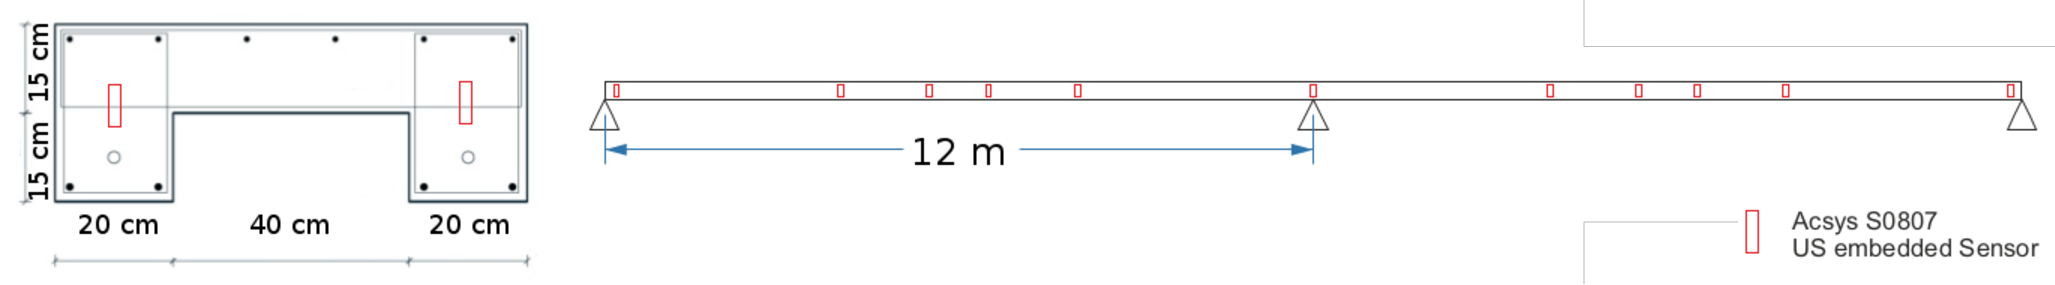
\includegraphics[width=0.95\linewidth]{Figures/BAM_bridge.pdf}};
		\node[anchor=south west,inner sep=0] (image) at (0.5,-2.5) 	{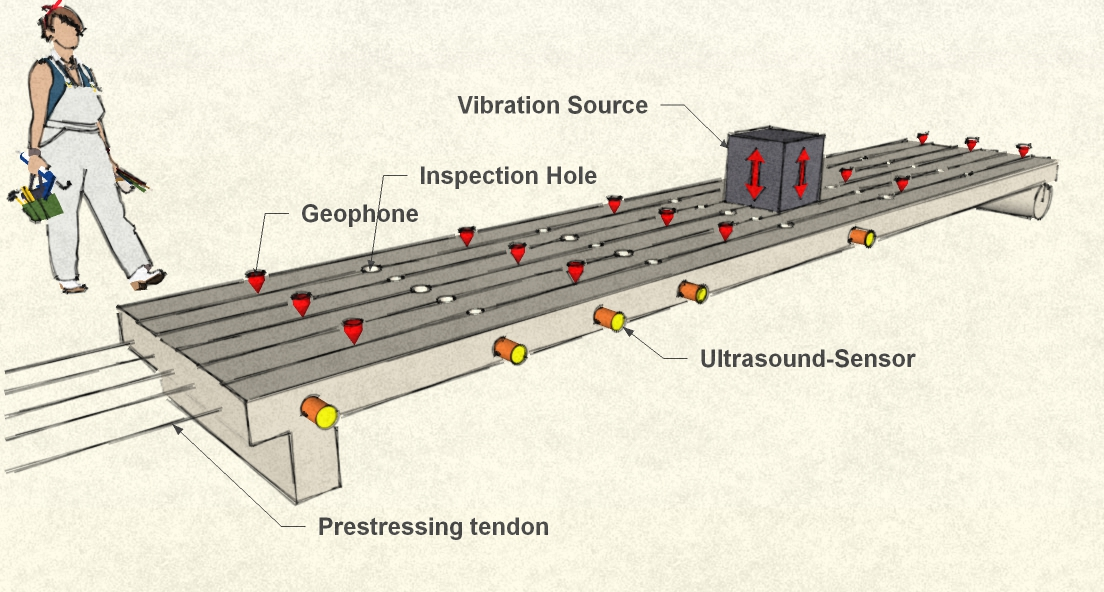
\includegraphics[width=0.6\linewidth]{Figures/TU-plate2.jpg}}; 
		\node[anchor=south west,inner sep=0] (image) at (0,-4.3) 	{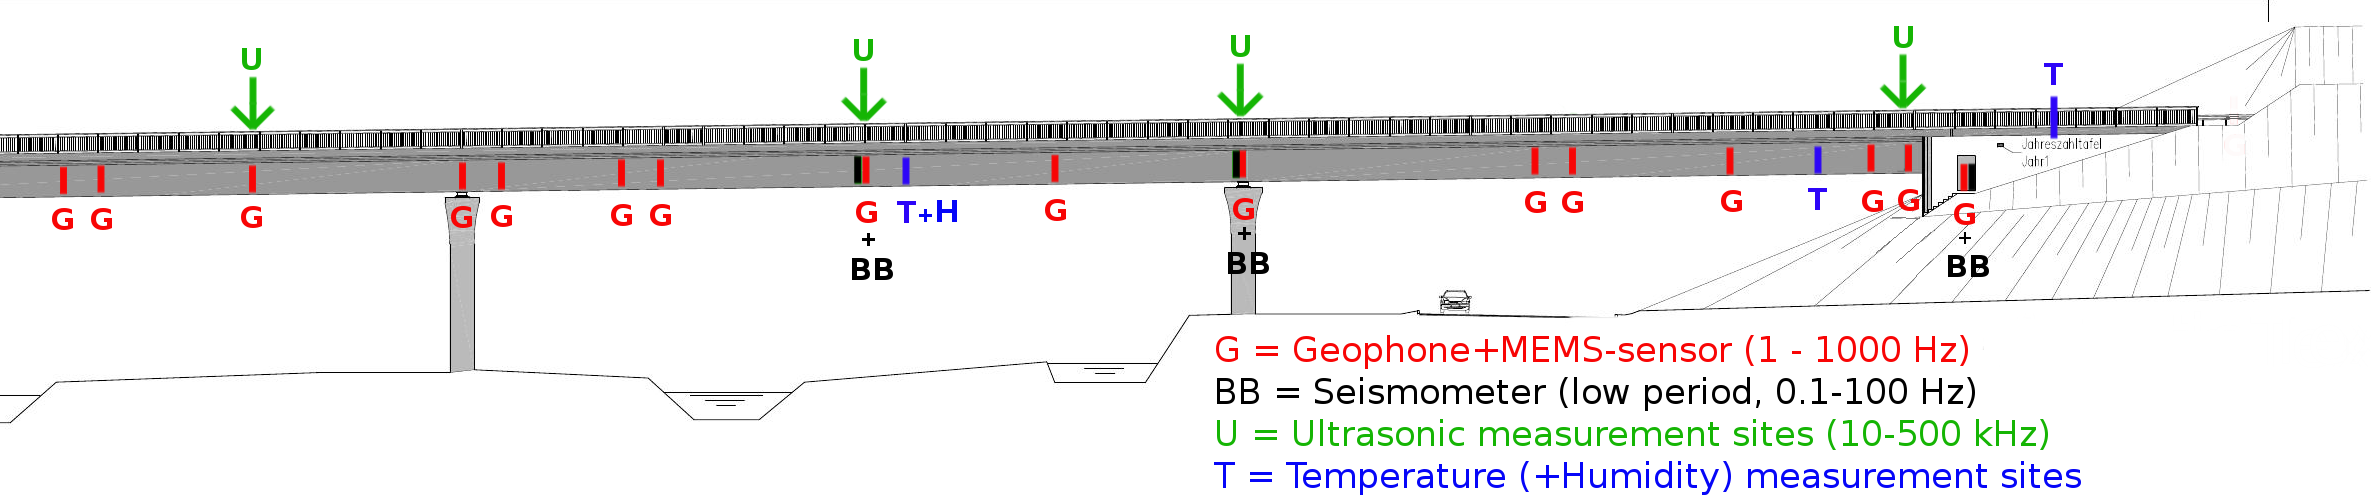
\includegraphics[width=0.7\linewidth]{Figures/bridge3.png}}; 
		\node[anchor=south west,inner sep=0] (image) at (8.5,-3.7) 	{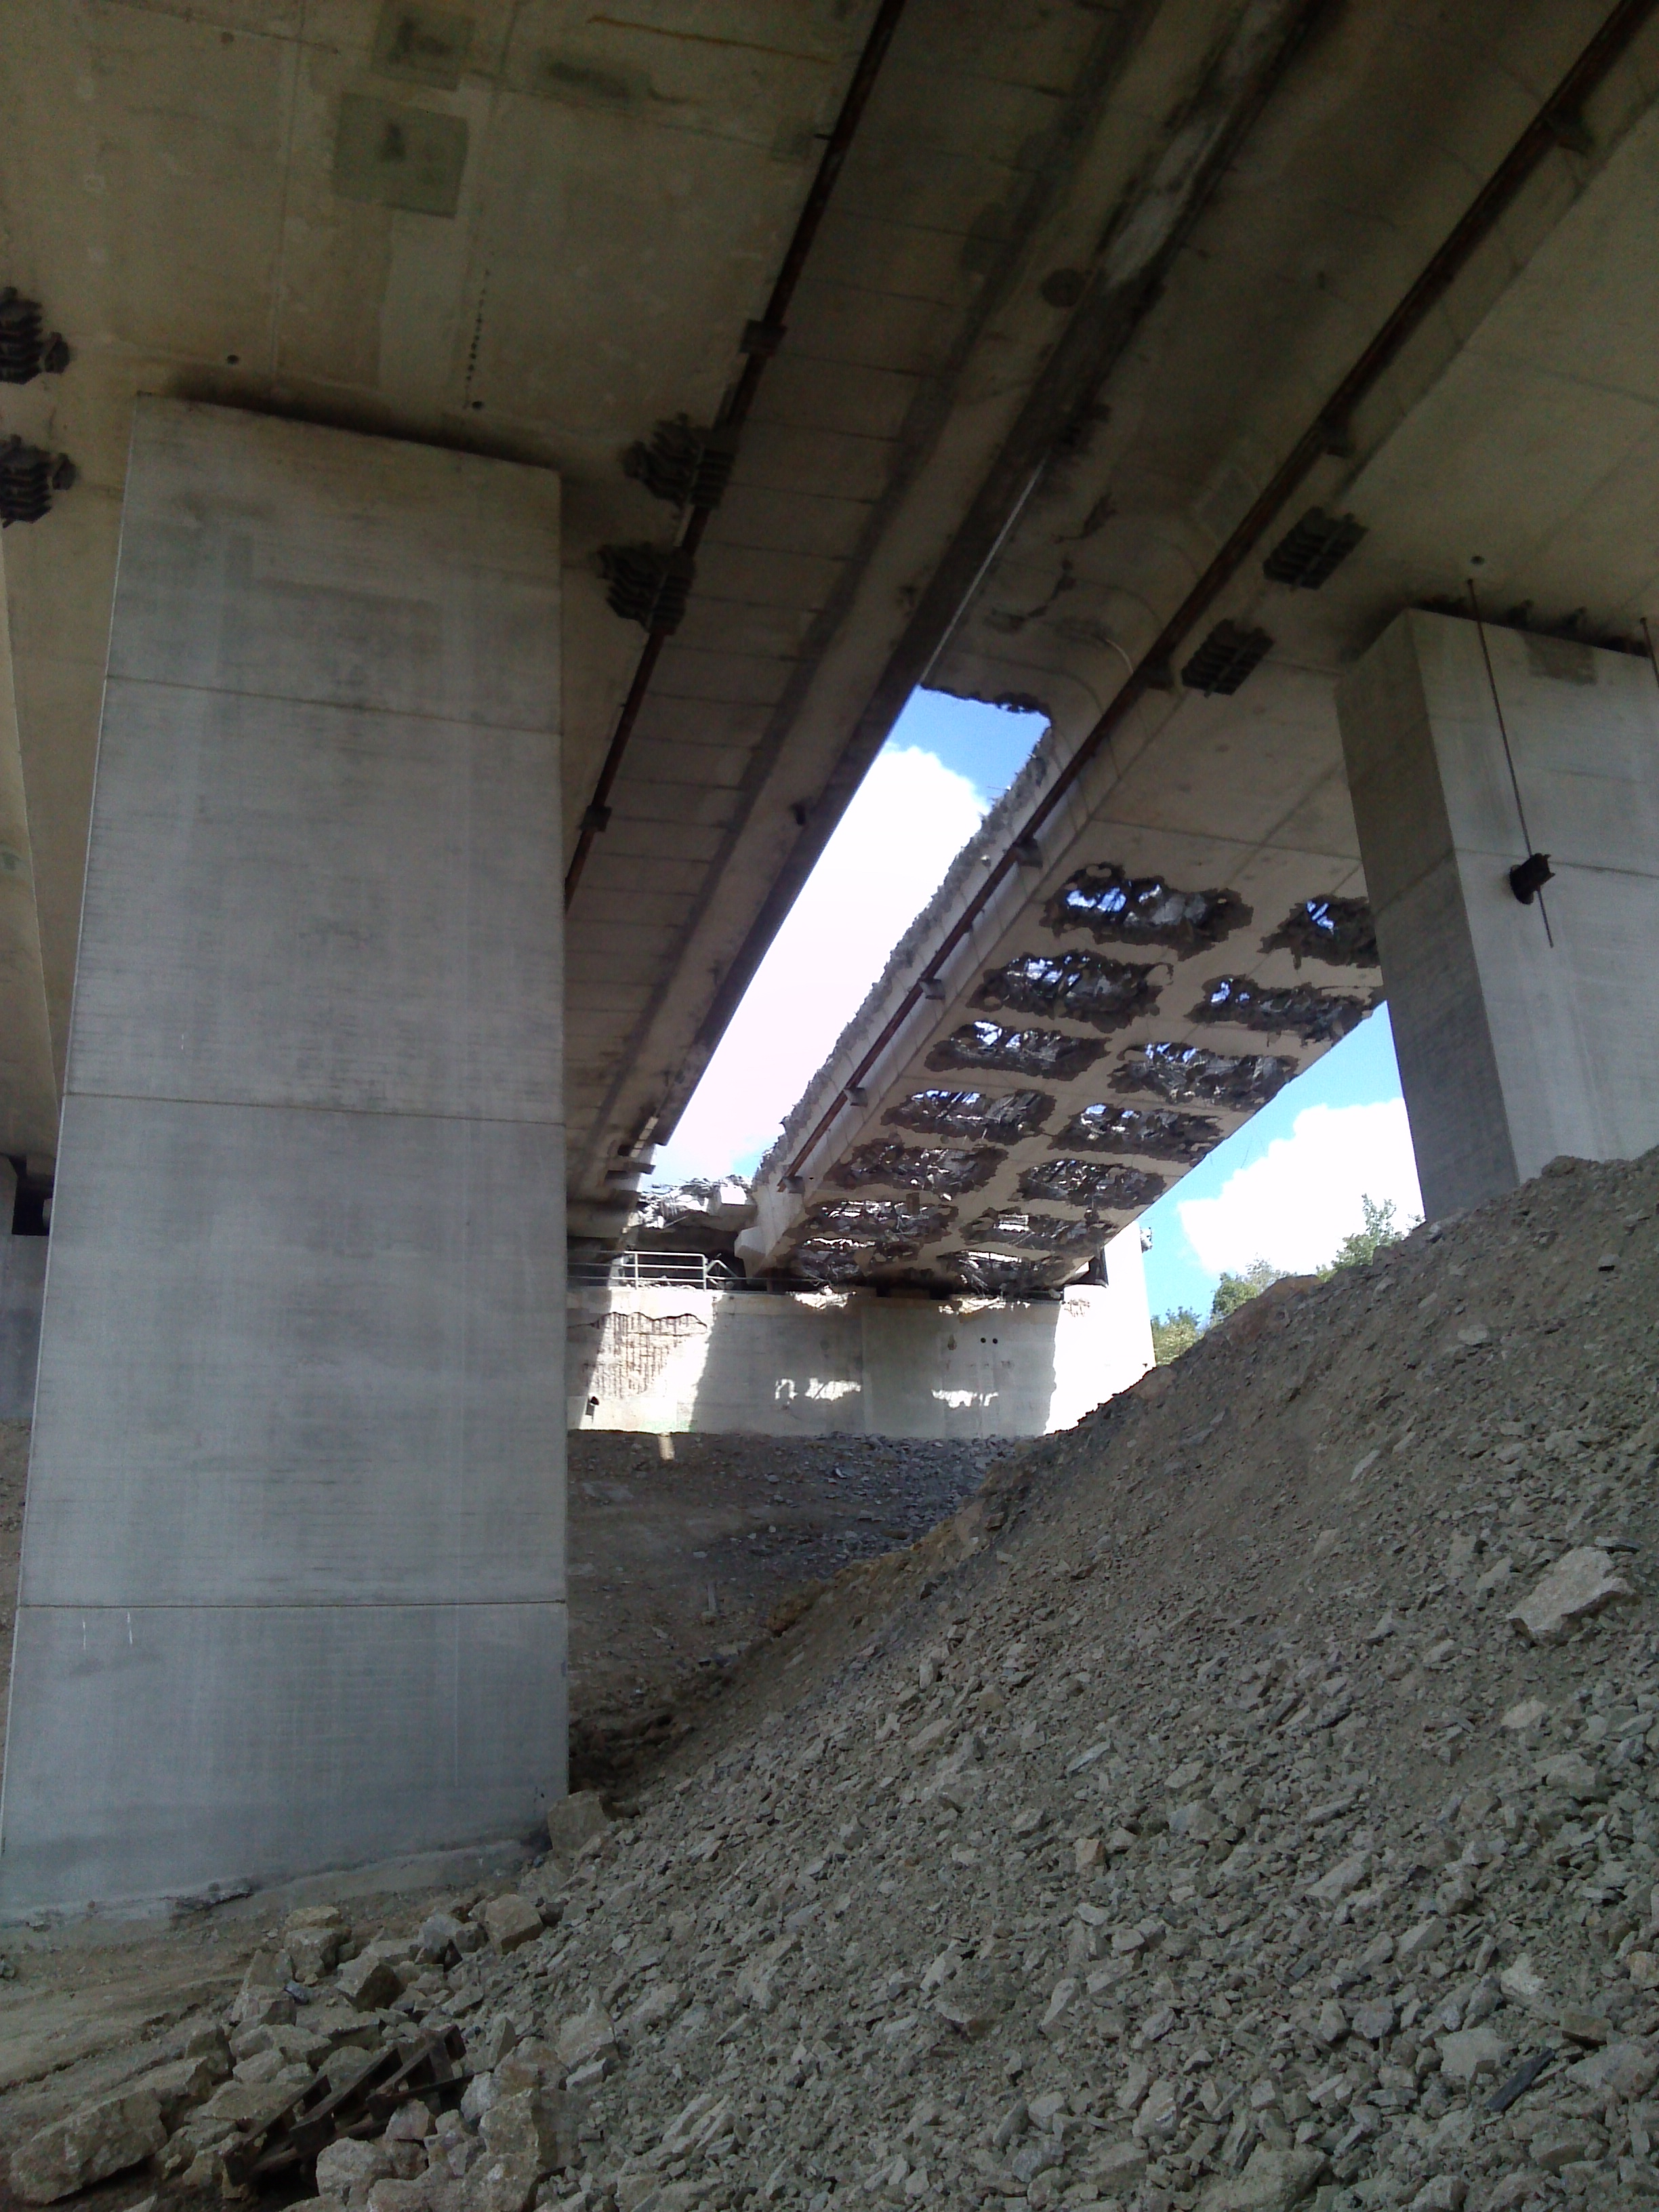
\includegraphics[width=0.3\linewidth]{Figures/abriss.jpg}};
	\end{tikzpicture}
\end{frame}

\begin{frame}
	\begin{tikzpicture}[overlay]
		\node[anchor=south west,inner sep=0] (image) at (0,1.5) 	{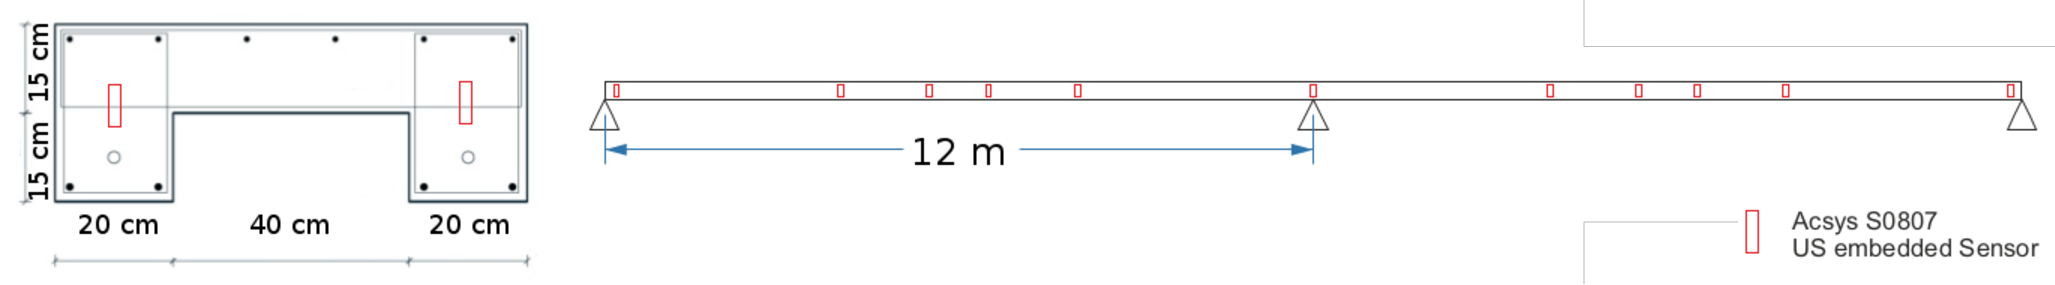
\includegraphics[width=0.95\linewidth]{Figures/BAM_bridge.pdf}};
		\node[anchor=south west,inner sep=0] (image) at (0.5,-2.5) 	{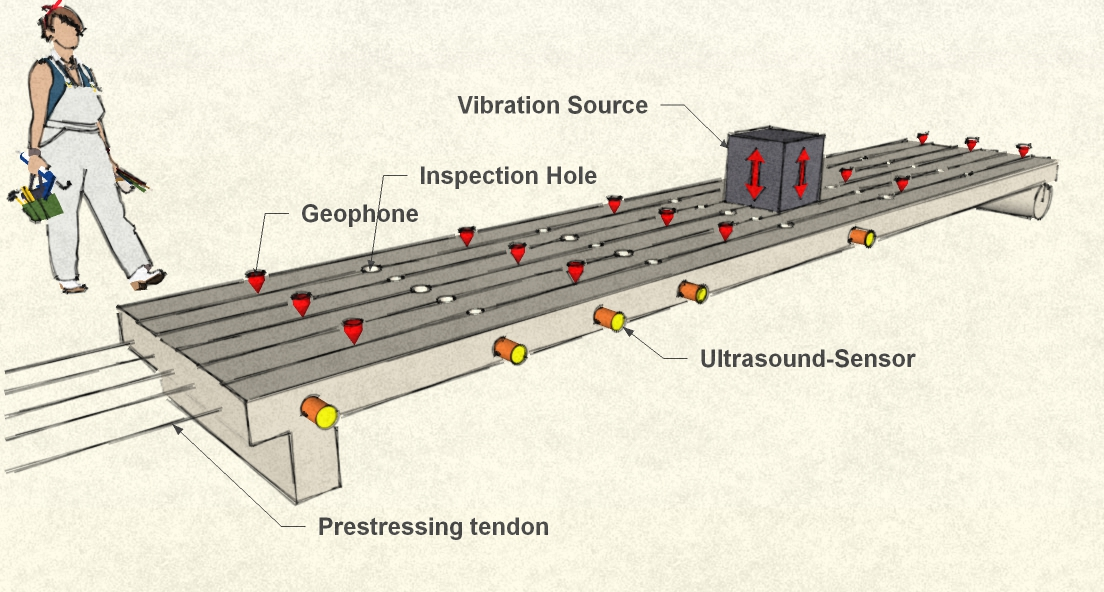
\includegraphics[width=0.6\linewidth]{Figures/TU-plate2.jpg}}; 
		\node[anchor=south west,inner sep=0] (image) at (0,-4.3) 	{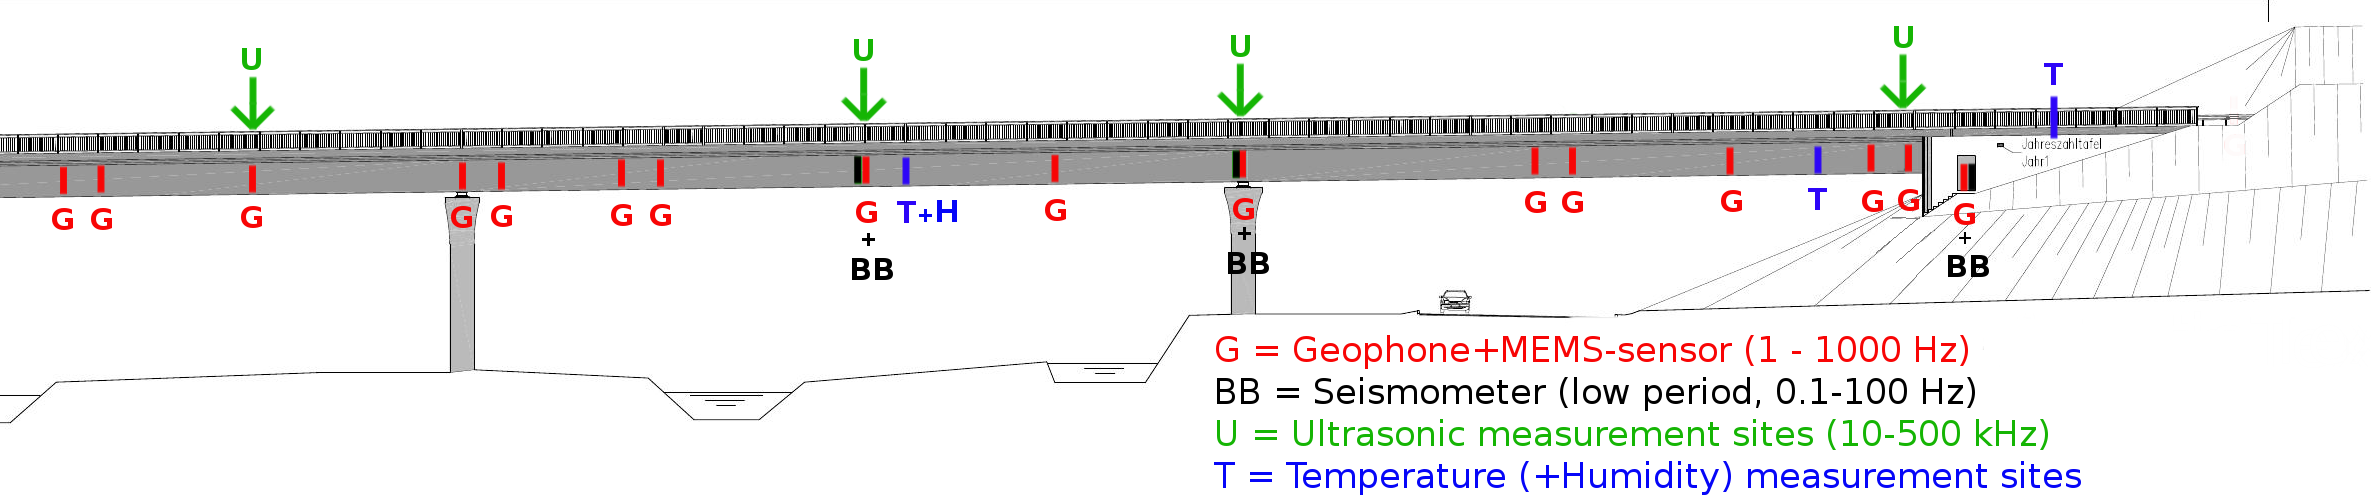
\includegraphics[width=0.7\linewidth]{Figures/bridge3.png}}; 
		\node[anchor=south west,inner sep=0] (image) at (8.5,-3.7) 	{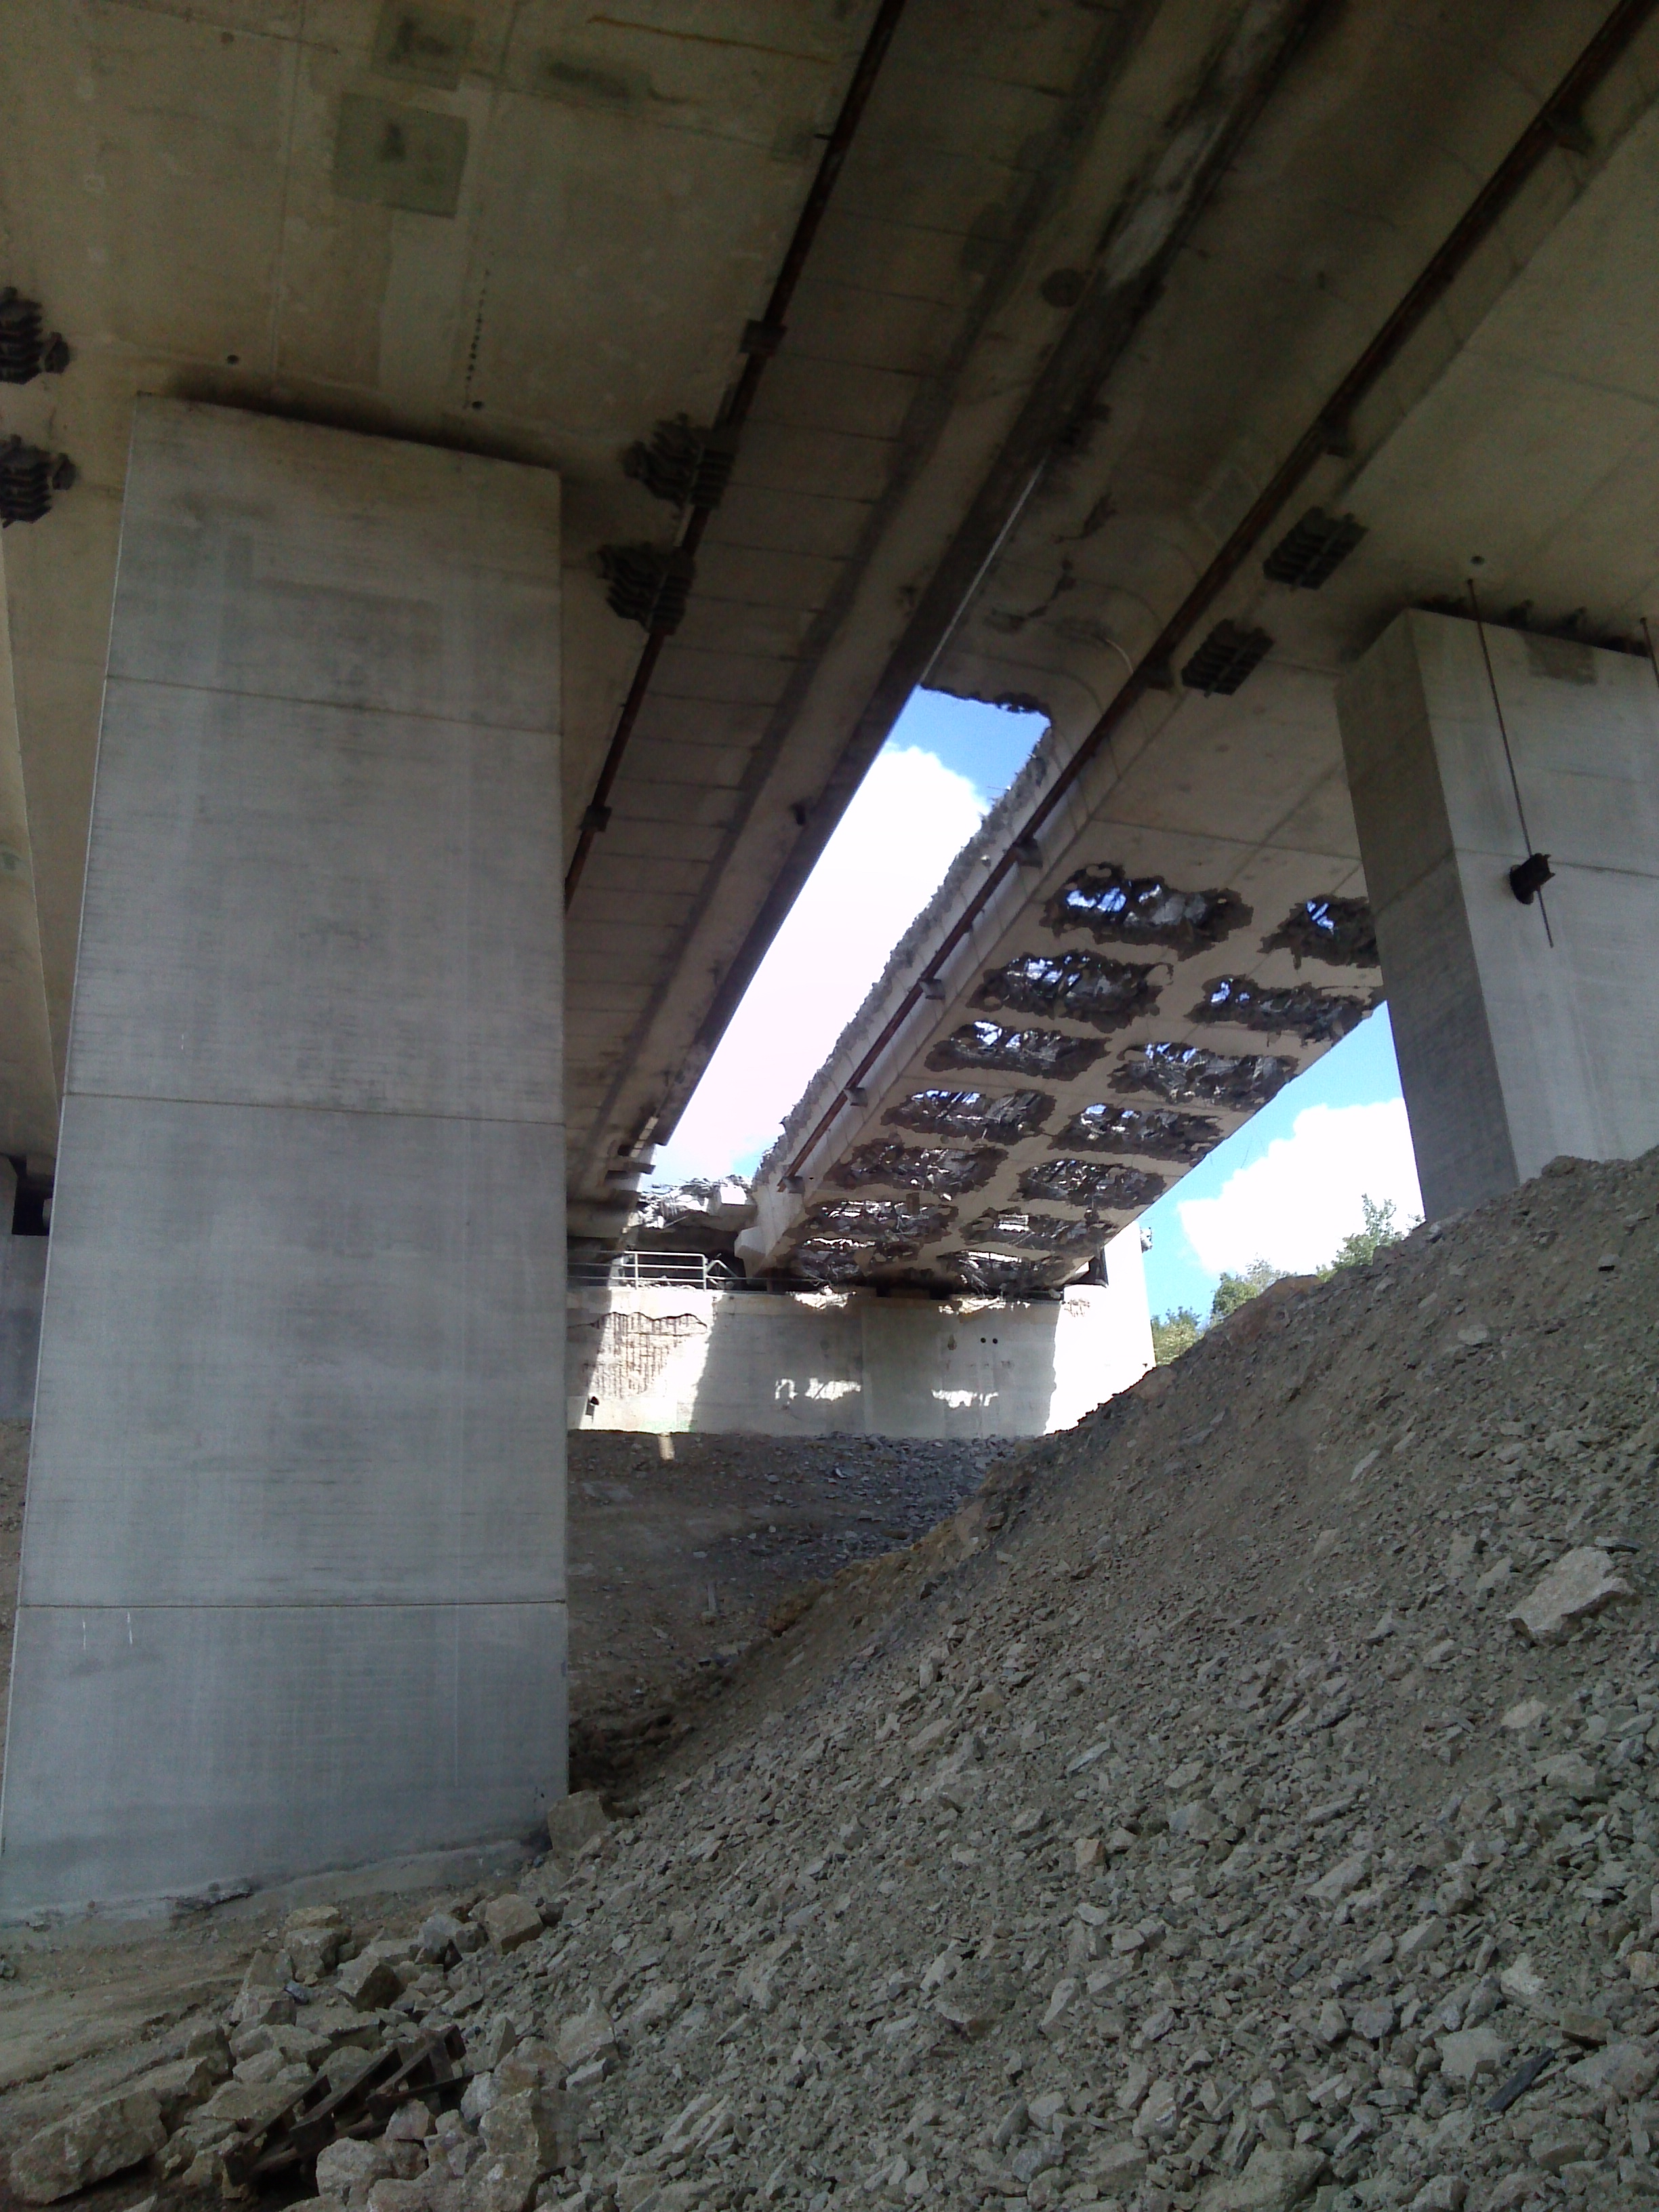
\includegraphics[width=0.3\linewidth]{Figures/abriss.jpg}};
		\node[anchor=south west,inner sep=0] (box2) at (1,-3) {
            		\begin{tcolorbox}[colback=green!5,colframe=salve@blue,title=Perspective - aspired project,width=10cm]
            		    \begin{small}
							\begin{itemize}
								\item Long-term ($>$ 1 year) monitoring of a highway bridge
								\item[] $\Rightarrow$ improve characterization of temperature effect  
								\item Extensive damage-scenario tests on sample bodies and expired structures
								\item Numerical simulations
								\item[] $\Rightarrow$ confirm reliability of damage detection
							\end{itemize}
            			\end{small}
					\end{tcolorbox}};
	\end{tikzpicture}
\end{frame}

\begin{frame}
	\begin{tikzpicture}[overlay]
		\node[anchor=south west,inner sep=0] (image) at (0,1.5) 	{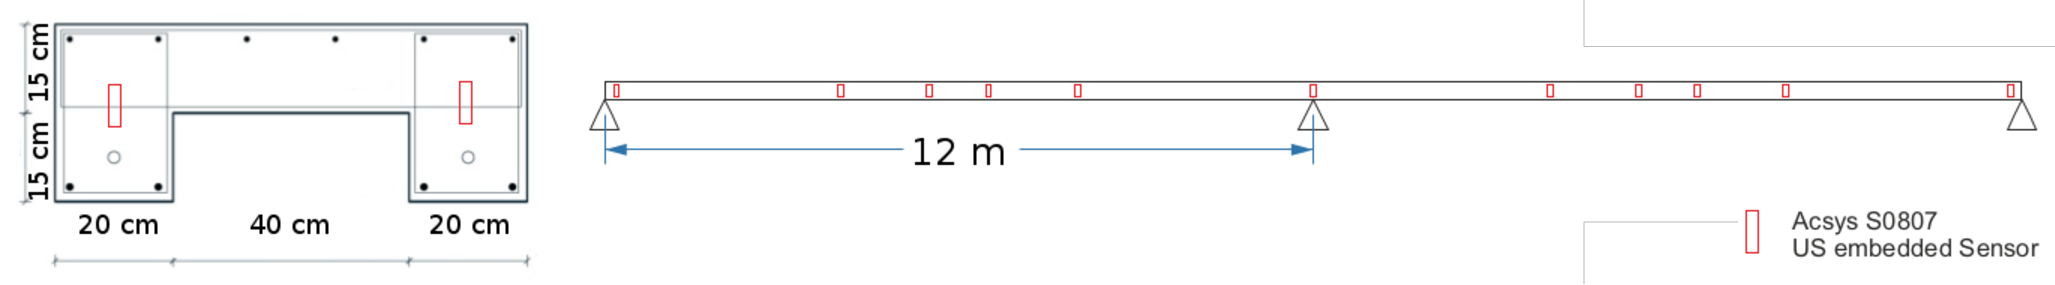
\includegraphics[width=0.95\linewidth]{Figures/BAM_bridge.pdf}};
		\node[anchor=south west,inner sep=0] (image) at (0.5,-2.5) 	{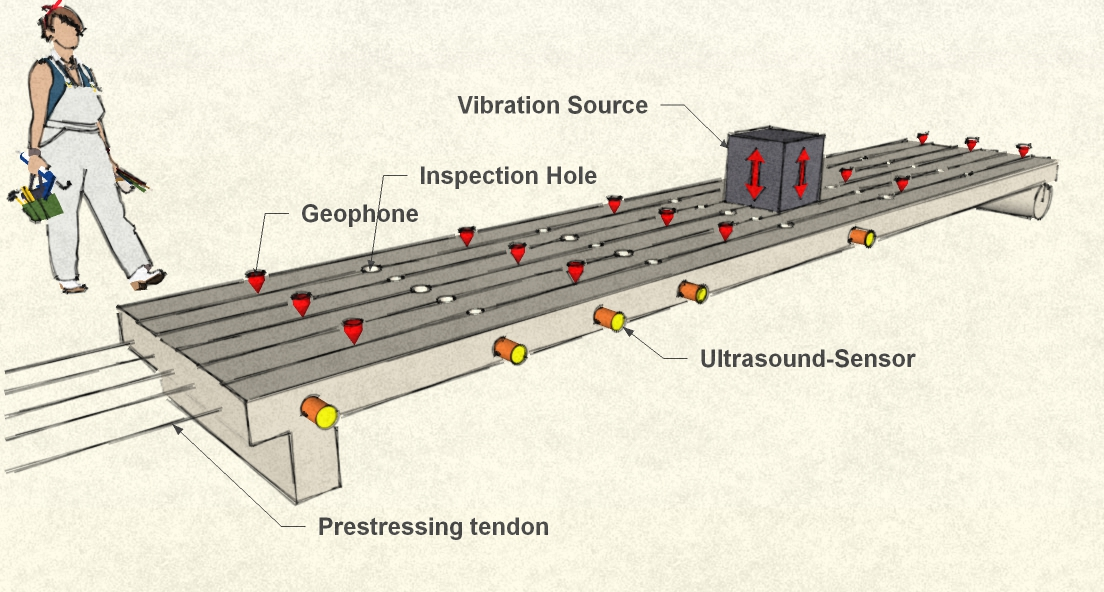
\includegraphics[width=0.6\linewidth]{Figures/TU-plate2.jpg}}; 
		\node[anchor=south west,inner sep=0] (image) at (0,-4.3) 	{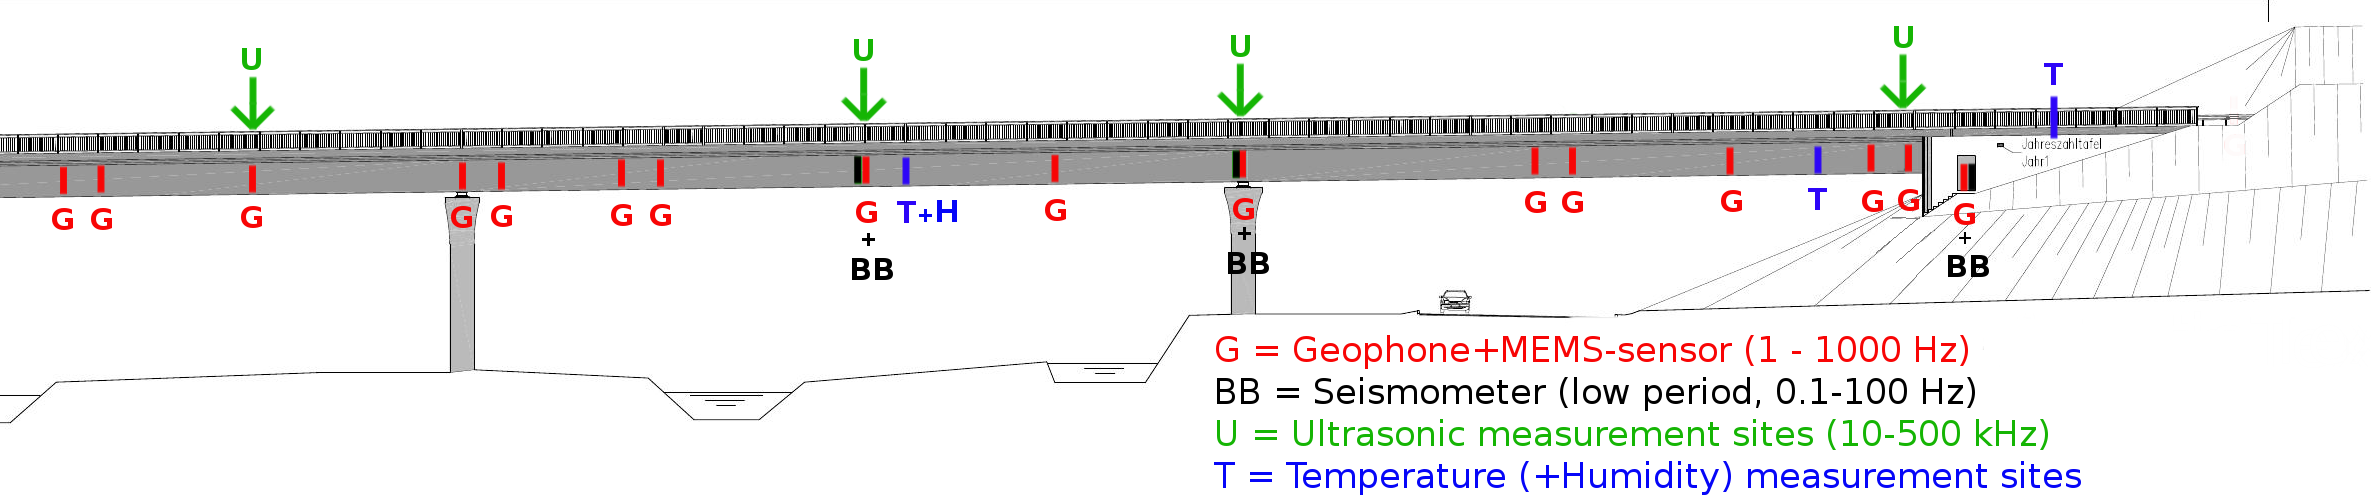
\includegraphics[width=0.7\linewidth]{Figures/bridge3.png}}; 
		\node[anchor=south west,inner sep=0] (image) at (8.5,-3.7) 	{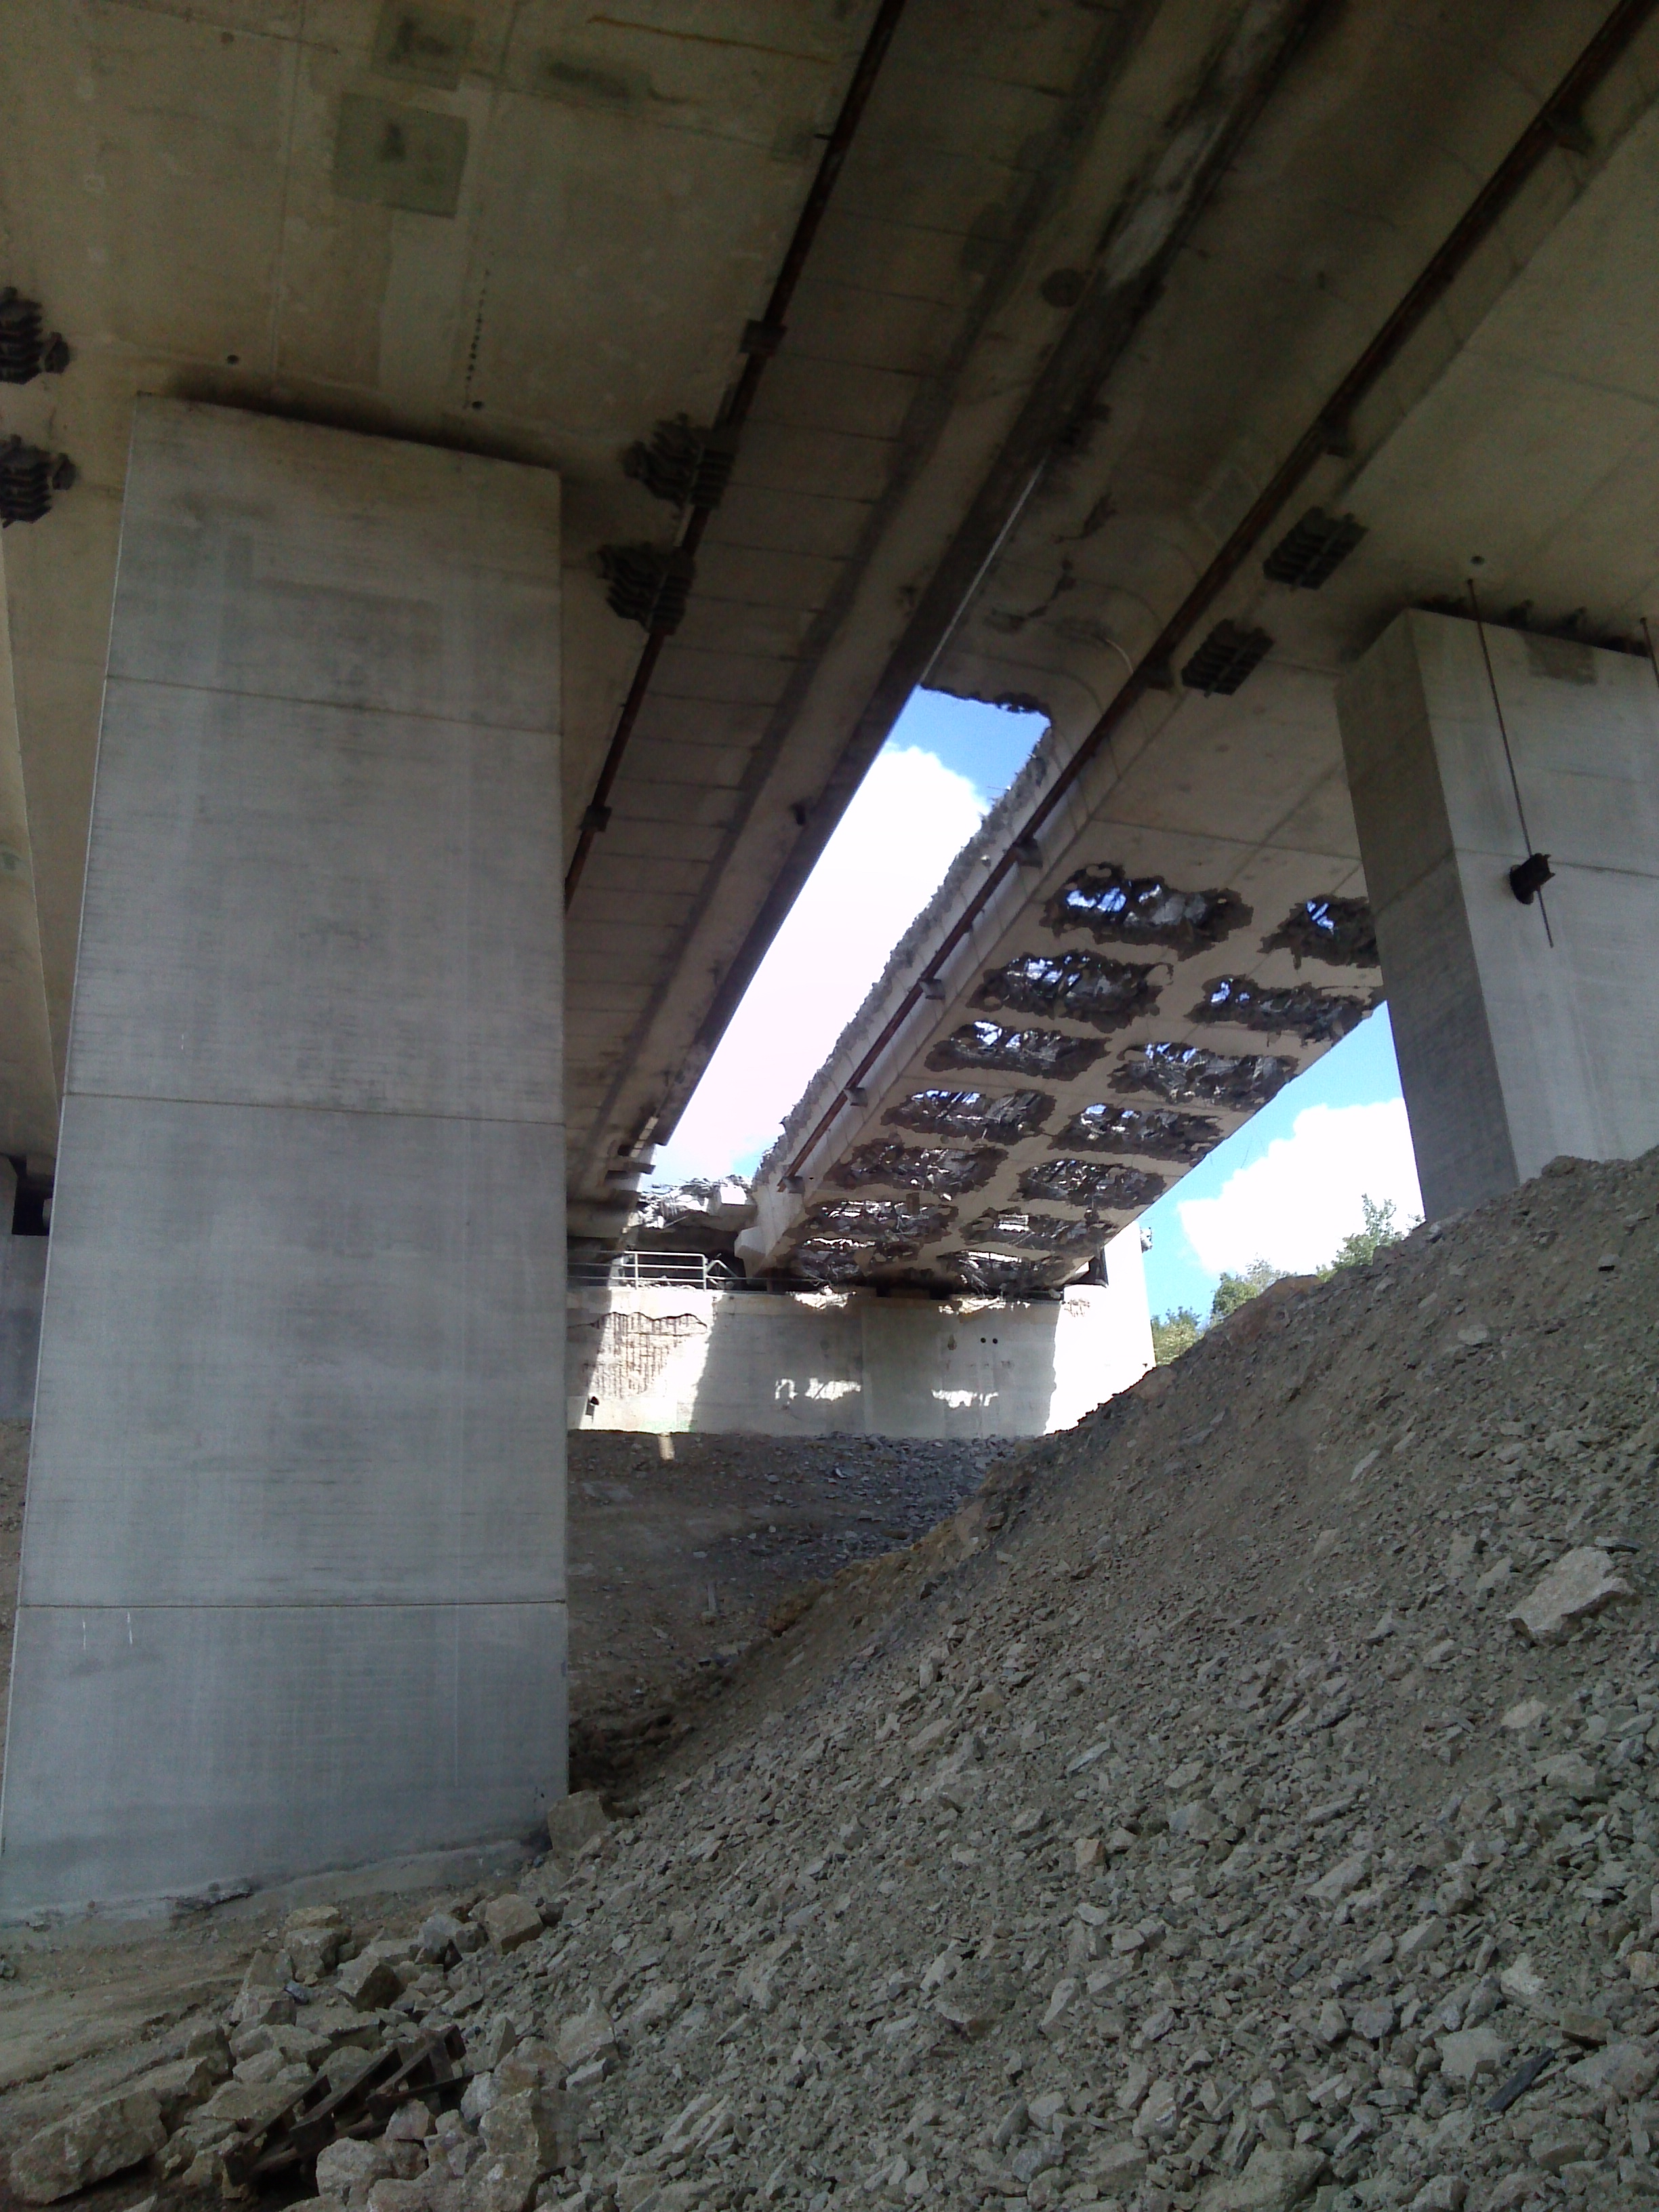
\includegraphics[width=0.3\linewidth]{Figures/abriss.jpg}};
		\node[anchor=south west,inner sep=0] (box2) at (1,-3) {
            		\begin{tcolorbox}[colback=green!5,colframe=salve@blue,title=Perspective - aspired project,width=10cm]
            		    \begin{small}
							\begin{itemize}
								{\color{green!5}\item[] Long-term ($>$ 1 year) monitoring of a highway bridge} 
								\item[] \textbf{Aim}
								\item[] Detect corrosion-induced \textbf{decrease in prestressing} and associated \textbf{concrete crack} evolution
								{\color{green!5}\item[] Numerical simulations
								\item[] $\Rightarrow$ confirm reliability of damage detection}
							\end{itemize}
            			\end{small}
					\end{tcolorbox}};
	\end{tikzpicture}
\end{frame}

%-------------------------------------------------------------------------------------------
%-------------------------------------------------------------------------------------------
%Questions slide

\begin{frame}
	\frametitle{Questions}
	\begin{center}
		\begin{tikzpicture}       
            \node[anchor=south west,inner sep=0] (image) at (-3,-2) {
\includegraphics[width=0.3\textwidth]{Figures/questions.jpeg}};
            \node[anchor=south west,inner sep=0] (thanks) at (1,1) {\textcolor{salve@blue}{\Huge{Thank you!}}};
         \end{tikzpicture}
    \end{center}
\end{frame}


%
% ============================================================================
\section{Extra}
\subsection{extra slides}

\begin{frame}
	\frametitle{Temperature reduction}
	\begin{center}
		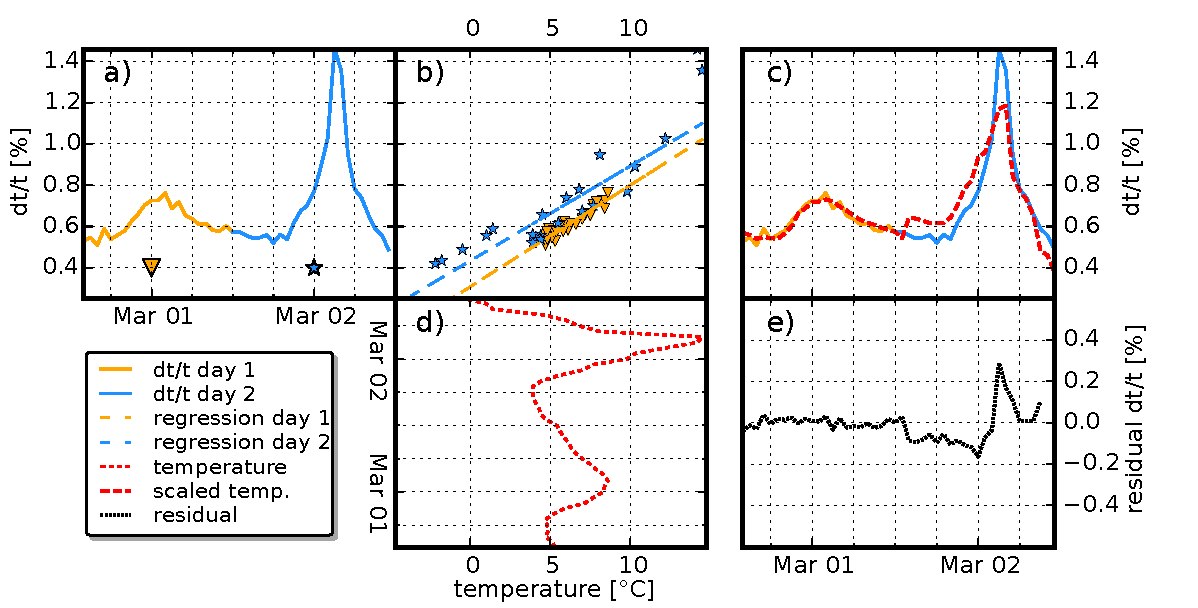
\includegraphics[width=\linewidth]{Figures/9.pdf}
    \end{center}
\end{frame}

\begin{frame}
	\frametitle{Daily Sunlight}
	\begin{center}
		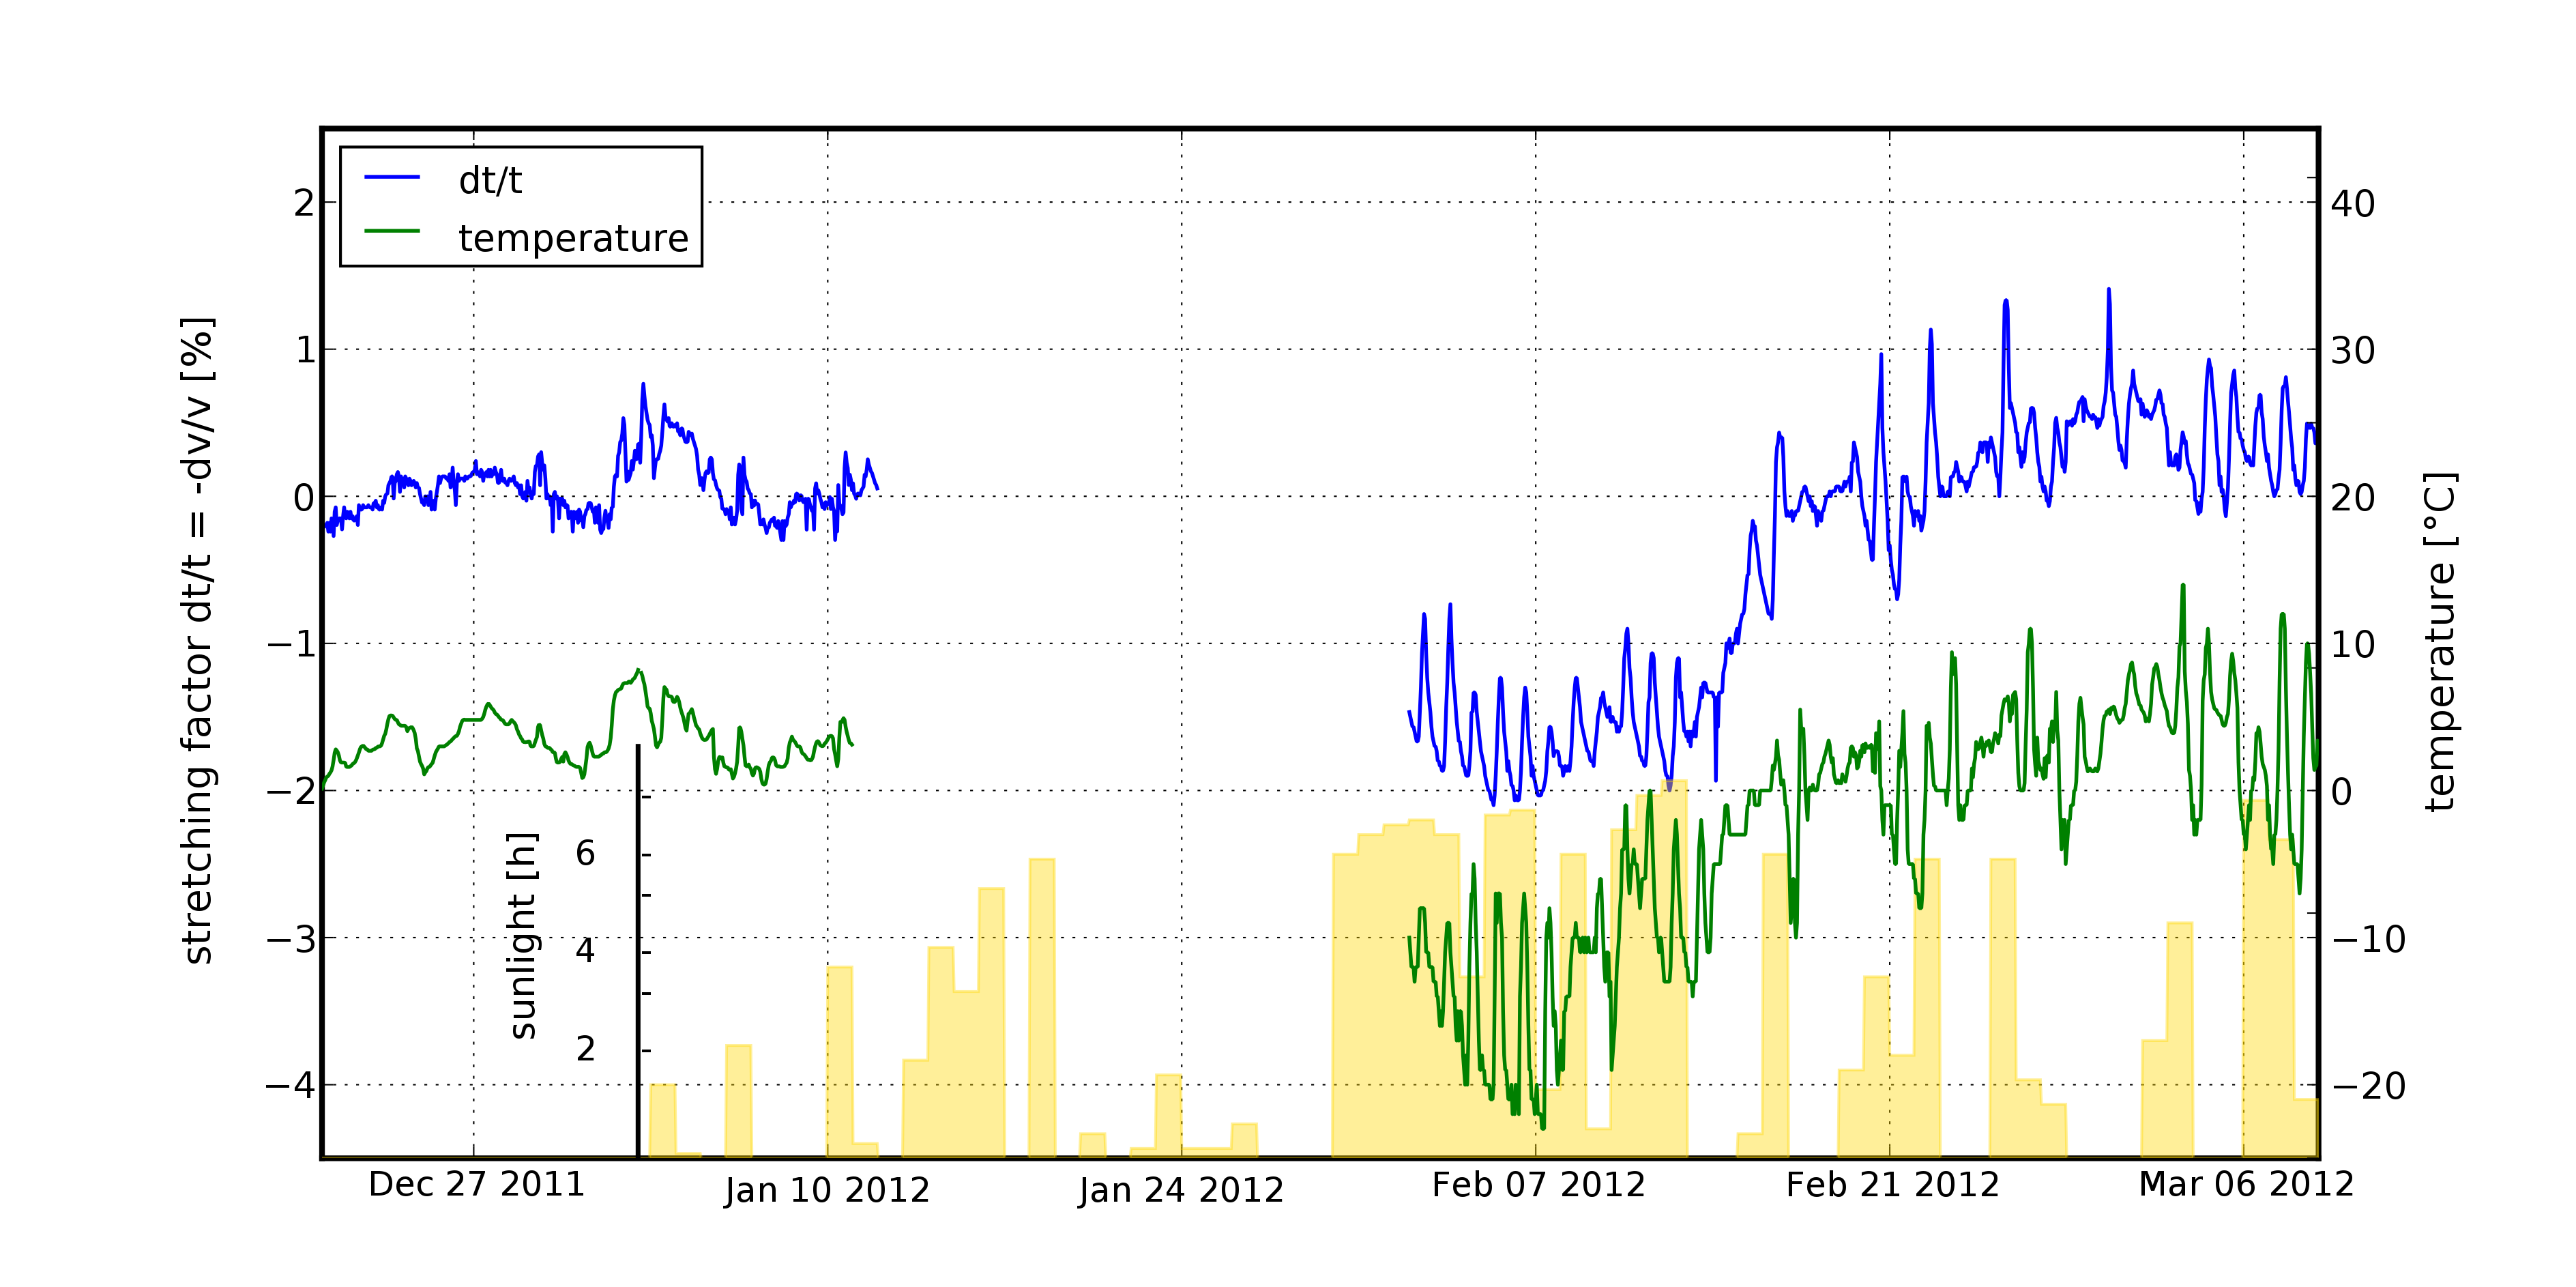
\includegraphics[width=\linewidth]{Figures/whole3.png}
    \end{center}
\end{frame}

\begin{frame}
	\frametitle{Stretching Method}
	\begin{center}
		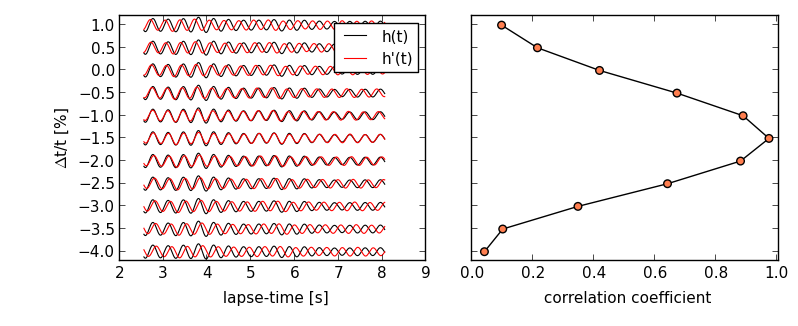
\includegraphics[width=\linewidth]{Figures/stretchingMethod.png}
    \end{center}
\end{frame}

\begin{frame}
	\frametitle{Eigenfrequency Evolution}
	\begin{center}
		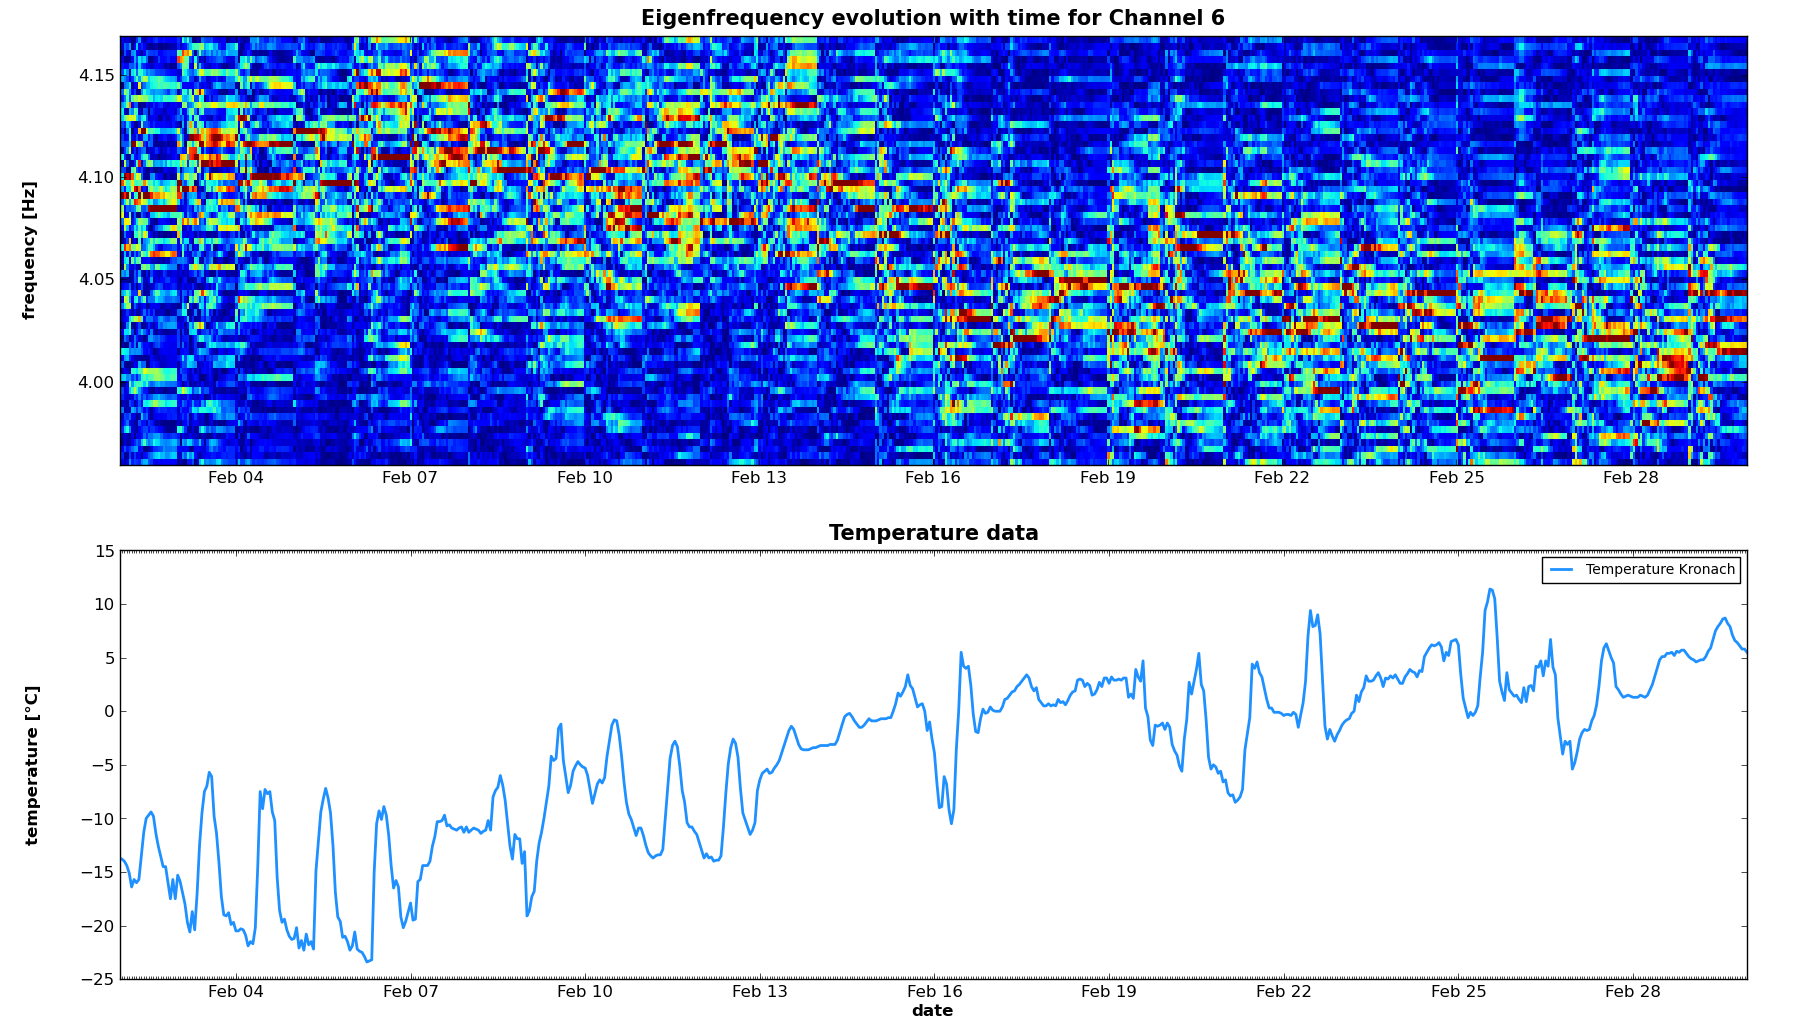
\includegraphics[width=\linewidth]{Figures/eigenfreq_evolution.png}
    \end{center}
\end{frame}

\begin{frame}
	\frametitle{Instrument Stability Test}
	\begin{center}
		\includegraphics[width=.85\linewidth]{Figures/freq_resp2.JPEG}
    \end{center}
\end{frame}
%
% =============================================================================
\end{document}
% =============================================================================
% EOF
% =============================================================================
